%% LaTeX_Thesis_Template.tex
% An unofficial LaTeX template for Cranfield theses.
% 2017/08/14 Daniel Auger's unofficial Cranfield thesis .sty file
% 2023/05/31 Updated by Shaun Forth (SAF) for logo inclusion
% 2023/06/08 SAF removed capitalisation on title pages on advice of Amy 
% Greenaway and Alison Waters. Added Daniel Auger's headers with 
% chapter and section names.
% 2023/06/08 SAF simplified logo inclusion

%%
% This document is an example of the use of the unofficial "cranfieldthesis" 
% LaTeX style file.  I hope it's useful, and a good likeness of the Word template.

\documentclass[12pt,oneside]{book} % for one-sided printing
%\documentclass[12pt,twoside]{book} % for two-sided printing

% Use the custom "cranfieldthesis" LaTeX style file. 
\usepackage{cranfieldthesis}
\usepackage{lscape} % for landscape pages
\usepackage{amsmath}
\usepackage{enumitem}
\usepackage{changepage}
\usepackage{pdfpages}
\usepackage{blindtext}% Just used so we can generate some example text
\usepackage{algorithm}
\usepackage{algpseudocode}
\usepackage{amssymb}
\usepackage{mathtools}
\usepackage[export]{adjustbox}
\usepackage{lipsum}
\usepackage{booktabs}  % For better quality tables
\usepackage{siunitx}
\usepackage{float}
\usepackage{longtable} % Pour les tableaux sur plusieurs pages
\usepackage{tabularx}  % for the X column type
\usepackage{listings}
\usepackage{xcolor}
\usepackage{caption}
\usepackage{xfrac}
\usepackage{indentfirst}
\usepackage{subcaption}
\usepackage{graphicx}
\usepackage{geometry}
\usepackage{titlesec}
\usepackage{multirow}
\usepackage{adjustbox} % To adjust the table size
\usepackage{arydshln}
\geometry{a4paper, margin=1in}
\hypersetup{
    colorlinks,
    linkcolor={blue!50!blue},
    citecolor={blue!50!blue},
    urlcolor={blue!80!blue}
}

% By default, LaTeX uses a serif font - these are traditionally thought to be
% easier to read.   If you'd prefer sans-serif, please uncomment the 
% following line.
% \renewcommand{\familydefault}{\sfdefault}

% Example parameters for a typical taught MSc course
\title{Future Position Prediction for Pressure Refuelling Port
    of Commercial Aircraft}
\author{Alexis Balayre}
\date{August 2024}
\school{\SATM}
\course{Computational and Software Techniques in Engineering}
\degree{MSc}
\academicyear{2023--2024}
\setCUPartnerLogo{logo-airbus.png}
\supervisors{Dr Boyu Kuang and Dr Stuart Barnes}
\copyrightyear{2024}

% References
% Cranfield Numbered Style
\usepackage[numbers]{natbib} % for nice referencing
\makeatletter % Reference list option change to number and period
\renewcommand\@biblabel[1]{#1.} % from [1] to 1
\makeatother %

\begin{document}
%% Front matter
%
% This is where we do the title page, etc.
%

\frontmatter

% Standard-Form Title Pages
\maketitle

% Abstract and Keywords
\begin{abstract}

    This thesis presents the development of a robust and efficient framework for
    predicting the future position of the pressure refuelling port of commercial
    aircraft. The proposed framework addresses critical challenges in automated
    aircraft refuelling systems, where accurate detection and prediction of the
    refuelling port's position are essential for operational efficiency and safety.
    Leveraging deep learning techniques, the framework integrates a fine-tuned
    YOLOv10 object detection model with a proposed sequence model, termed
    SizPos-GRU. This sequence model utilises an encoder-attention-decoder
    architecture to effectively capture temporal dependencies and spatial
    relationships from video frames. The methodology includes meticulous dataset
    configuration and annotation, followed by hyperparameter tuning to optimise
    model performance. Experimental results demonstrate the SizPos-GRU model's
    superior predictive accuracy across different scenarios. Specifically, the
    Savitzky-Golay filter combined with a Linear Kalman Filter (LKF) yielded the
    best performance, achieving an Average Displacement Error (ADE) of 32.45 pixels
    and a Final Displacement Error (FDE) of 57.98 pixels in the
    \textit{video\_lab\_platform\_6} dataset. Additionally, the model achieved a
    Final Intersection over Union (FIoU) of 28.27\%, highlighting its ability to
    maintain spatial overlap between predicted and actual positions. In other
    datasets, such as \textit{test\_indoor1}, the framework demonstrated consistent
    performance with an ADE of 76.48 pixels and an FDE of 127.81 pixels when using
    the Savitzky-Golay filter without LKF. These findings underscore the potential
    of the proposed framework to significantly improve the automation of aircraft
    ground operations, making a valuable contribution to the field by advancing the
    state-of-the-art in predictive modelling for dynamic environments.

\end{abstract}

\begin{keywords}
    Aircraft Refuelling Port Detection, Spatio-temporal Prediction, Deep Learning Sequence Models, \textit{SizPos-GRU} model, Kalman Filtering, Savitzky-Golay Smoothing
\end{keywords}

% Acknowledgements
\chapter{Acknowledgements}
I would like to express my deepest gratitude to my supervisors, Dr. Boyu Kuang
and Dr. Stuart Barnes, for their invaluable guidance, encouragement, and
support throughout this research. I am especially grateful to Dr. Boyu Kuang,
whose unwavering dedication, insightful feedback, and willingness to go the
extra mile have been instrumental in overcoming the challenges faced during
this study. His mentorship has not only greatly enriched the quality of this
thesis but also inspired me to pursue excellence in my research. I also wish to
acknowledge the use of ChatGPT, an AI language model by OpenAI, which provided
assistance in refining the language and clarity of this thesis. As a non-native
English speaker, this support was instrumental in ensuring the quality of the
writing. I am also grateful to Dr. Muhammad Monjurul Karim, Postdoctoral
Scholar at the University of Washington, for providing access to the source
code of the Fusion-GRU model~\cite{FusionGRU}, which was pivotal in the
development of this research. Additionally, I would like to extend my
appreciation to Airbus, the UK Research and Innovation (UKRI) and the Aerospace
Technology Institute (ATI) for sponsoring this research through the ONEheart
project. Finally, my heartfelt thanks go to my family and friends for their
unwavering support and understanding during my studies.

    { \clearpage

        % Table of Contents
        \singlespacing{
            \tableofcontents
        }
        \clearpage

        % List of Figures
        {%
            \let\oldnumberline\numberline%
            \renewcommand{\numberline}{\figurename~\oldnumberline}%
            \listoffigures%
        }

        \clearpage
        % List of Tables
        {%
            \let\oldnumberline\numberline%
            \renewcommand{\numberline}{\tablename~\oldnumberline}%
            \listoftables%
        }
    }

% The list of abbreviations can't be automatically generated so you need to populate it yourself
\begin{listofabbreviations}
    \abbrev{AAGR}{Autonomous Aircraft Ground Refuelling}
    \abbrev{ADE}{Average Displacement Error}
    \abbrev{AFRL}{Air Force Research Laboratory}
    \abbrev{AI}{Artificial Intelligence}
    \abbrev{AAR}{Autonomous Aerial Refuelling}
    \abbrev{AIoU}{Average Intersection over Union}
    \abbrev{AP}{Average Precision}
    \abbrev{AR}{Average Recall}
    \abbrev{AR3P}{Autonomous \& Robotic Remote Refuelling Point}
    \abbrev{CNN}{Convolutional Neural Network}
    \abbrev{CV}{Constant Velocity}
    \abbrev{DGPS}{Differential Global Positioning System}
    \abbrev{DL}{Deep Learning}
    \abbrev{EKF}{Extended Kalman Filter}
    \abbrev{FDE}{Final Displacement Error}
    \abbrev{FIoU}{Final Intersection over Union}
    \abbrev{GPS}{Global Positioning System}
    \abbrev{GRU}{Gated Recurrent Unit}
    \abbrev{HOG}{Histogram of Oriented Gradients}
    \abbrev{IoT}{Internet of Things}
    \abbrev{IoU}{Intersection over Union}
    \abbrev{LKF}{Linear Kalman Filter}
    \abbrev{LSTM}{Long Short-Term Memory}
    \abbrev{ML}{Machine Learning}
    \abbrev{NMS}{Non-Maximum Suppression}
    \abbrev{PV-LSTM}{Pedestrian Intention Prediction LSTM}
    \abbrev{RNN}{Recurrent Neural Network}
    \abbrev{SOTA}{State-of-the-Art}
    \abbrev{SSD}{Single Shot Multibox Detector}
    \abbrev{STED}{Spatio-Temporal Encoder-Decoder}
    \abbrev{UAV}{Unmanned Aerial Vehicle}
    \abbrev{YOLO}{You Only Look Once}
\end{listofabbreviations}

%% Main Matter
%
% This is where we include the main thesis content.
%
\mainmatter\pagestyle{fancy}
\fancyhead[L]{\nouppercase{\leftmark}}
\fancyhead[R]{\nouppercase{\rightmark}}

%%%%%%%%%%%%%%%%%%%%%%%%%%%%%%%%%%%%%%%%%%%%%%%%%%%%%%%%%%%%%%%%%%%%%%%%%%%%%%%%
%%%%%%%%%%%%%%%%%%%%%%%%%%%%%%%%% INTRODUCTION %%%%%%%%%%%%%%%%%%%%%%%%%%%%%%%%%
\chapter{Introduction}
\section{Background and Motivation}

Ground pressure refuelling is a standard method used to refuel commercial
aircraft safely and efficiently. This process involves using a system of
underground fuel pipelines and hydrants at aircraft parking
spots~\cite{blakey2011aviation}. When an aircraft is ready for refuelling, a
hydrant dispenser vehicle connects to the hydrant pit and delivers fuel to the
aircraft through a flexible hose~\cite{sati2019aircraft} (see
Figure~\ref{fig:pressure-refuelling}). This method allows for high fuel flow
rates and significantly reduces aircraft turnaround
times~\cite{blakey2011aviation}. However, this process also presents several
challenges, particularly in terms of safety and accuracy. In the past, there
have been several incidents involving ground pressure refuelling, including
fuel spills, overfills, and equipment
failures~\cite{doi:10.1080/13669877.2013.879493, CostsOfUnsafetyAviation}.
Fortunately, with the advancement of technology, many of these challenges will
be addressed, and the refuelling process will become safer and more efficient. 

\begin{figure}[H]
    \centering
    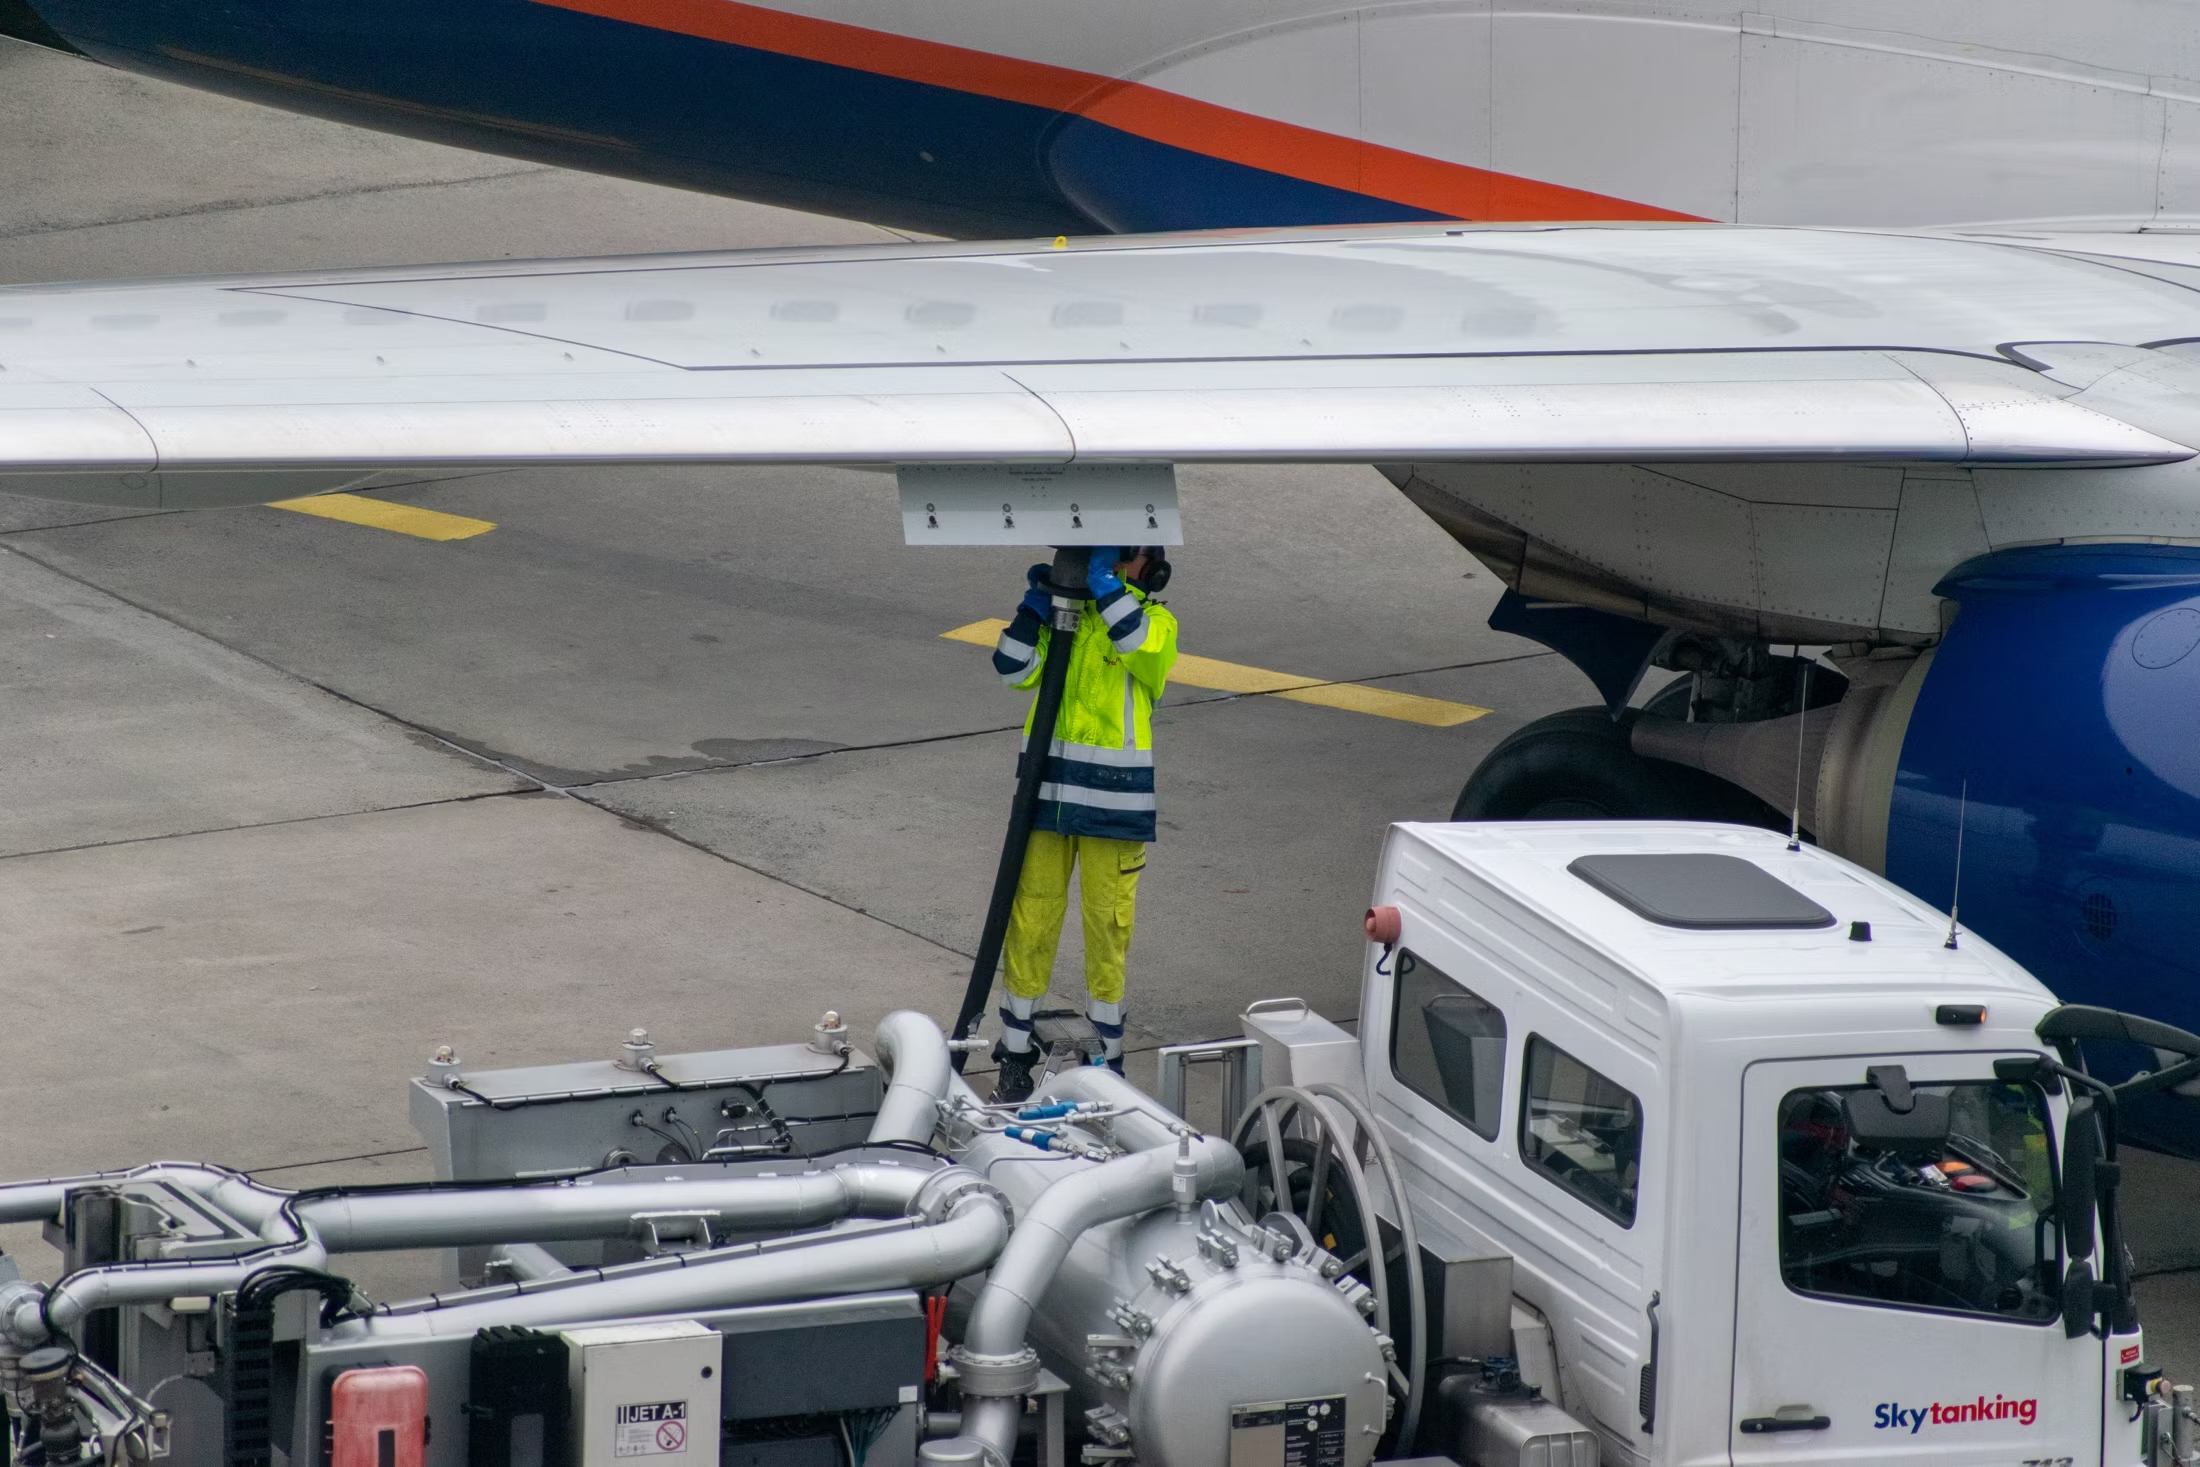
\includegraphics[width=0.5\textwidth]{figures/pressure-refuelling.jpeg}
    \caption{Pressure Refuelling of a Commercial Aircraft. Photo Credit: Tom Boon/Simple Flying~\cite{ImageRefueling}}\label{fig:pressure-refuelling}
\end{figure}

The aviation industry is undergoing a significant transformation with the
development of the airport of the future, commonly known as `Smart Airport’ or,
more recently, `Airport 4.0’. The concept of Smart Airport encompasses the use
of cutting-edge information technologies, such as the Internet of Things (IoT),
Artificial Intelligence (AI), and Blockchain, to monitor, analyse, and
integrate real-time data on the airport's status. This integration aims to
achieve optimal operational efficiency and enhance the quality of service.
Taking the concept a step further, Airport 4.0 envisages an airport driven
entirely by AI, capable of making autonomous decisions thanks to self-learning
mechanisms. This advance aims to automatically predict and manage various
airport scenarios, making it easier to automate numerous processes. The result
is a substantial reduction in operating costs and error
rates~\cite{10.1007/978-981-16-5943-0_26}.

Among these, automated refuelling systems play a crucial role in ensuring
efficient and accurate refuelling of aircraft. However, one of the main
challenges of this automation process is the accurate detection of the
aircraft's refuelling port, which is relatively small and can easily be
obscured by other visual elements on or near an aircraft. For example in the
Figure~\ref{fig:challenges-detecting-ports}, the refuelling port is located on
the wing of the aircraft and can be difficult to detect due to motion blur,
occlusion, or being out of view. This challenge is further compounded by the
fact that aircraft refuelling ports can vary in size, shape, and location
depending on the aircraft type and manufacturer. Scanning the entire area of
each video frame is both time-consuming and inaccurate. It is therefore
essential to develop a more efficient and accurate method of locating the
refuelling port. 

% 4 Images
\begin{figure}[H]
    \centering
    \begin{subfigure}[b]{0.3\textwidth}
        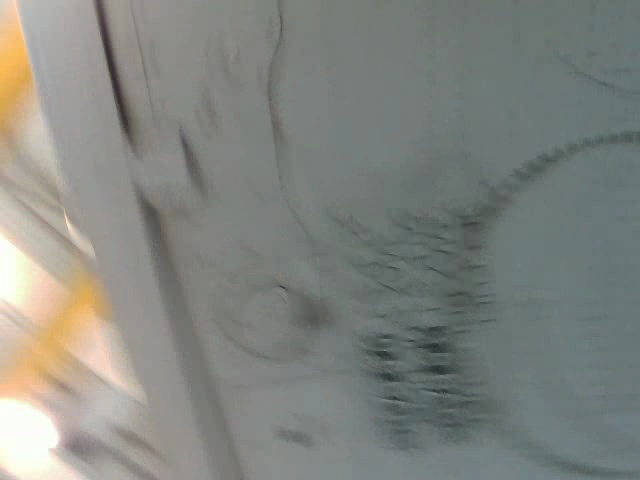
\includegraphics[height=0.7\textwidth, width=\textwidth]{figures/image_hard_2.jpg}
        \caption{Motion Blur Example}\label{fig:motion-blur-example}
    \end{subfigure}
    \hfill
    \begin{subfigure}[b]{0.3\textwidth}
        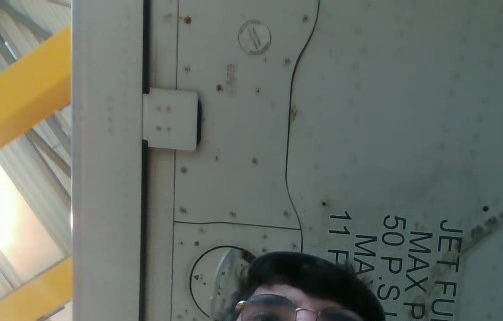
\includegraphics[height=0.7\textwidth, width=\textwidth]{figures/image_hard_4.jpg}
        \caption{Occlusion Example}\label{fig:occlusion-example}
    \end{subfigure}
    \hfill
    \begin{subfigure}[b]{0.3\textwidth}
        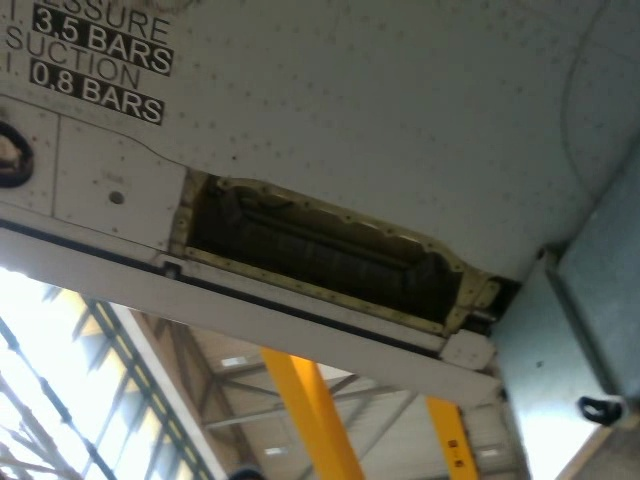
\includegraphics[height=0.7\textwidth, width=\textwidth]{figures/image_hard_3.jpg}
        \caption{Out-of-View Example}\label{fig:out-of-view-example}
    \end{subfigure}
    \caption{Challenges in Detecting Aircraft Refuelling Port}\label{fig:challenges-detecting-ports}
\end{figure}

\section{Research Gap}
Despite significant advancements in autonomous aircraft ground refuelling
technologies, critical challenges remain, particularly in the accurate
detection and positioning of the refuelling port. The small size and varied
locations of refuelling ports, often obscured by visual elements like motion
blur and occlusions, complicate this task. Existing systems have made progress
using machine vision, but they are limited by inefficiencies in scanning entire
video frames and inaccuracies under different environmental conditions.
Furthermore, while current methodologies leveraging convolutional neural
networks (CNNs) and Kalman filters have improved detection accuracy, they still
struggle with real-time performance and adaptability in dynamic environments.
The robustness of these systems in varied lighting conditions and their
capability to handle different refuelling port types and obstructions need
enhancement. Additionally, the application of advanced deep learning models
like Long Short-Term Memory (LSTM) networks, Gated Recurrent Units (GRUs), and
Transformers in this context is underexplored. 

\section{Aim and Objectives}
This thesis aims to address the previous research gaps by developing a
framework for predicting the future position of commercial aircraft refuelling
ports using advanced Object Detection models and Deep Learning to leverage the
spatial-temporal relationship between frames in a video.
\begin{enumerate}
    \item Conduct a comprehensive review of state-of-the-art methods for Object
          Detection, Object Tracking, and Deep Learning Sequence Models.
    \item Annotate and preprocess video datasets of aircraft refuelling ports to ensure
          high-quality training and testing data.
    \item Design and develop a framework for accurately tracking and predicting the
          future position of aircraft refuelling ports.
\end{enumerate}

\section{Technological Contributions}
This thesis presents significant technological contributions that advance the
field of automated aircraft refuelling and predictive modelling. The primary
contribution is the development of the \textit{SizPos-GRU} model, a novel deep
learning sequence model designed to accurately predict the future positions of
aircraft refuelling ports in dynamic video sequences. The \textit{SizPos-GRU}
model employs an encoder-attention-decoder architecture that effectively
captures temporal dependencies and spatial relationships from video frames,
resulting in superior predictive accuracy when compared to existing models. In
addition to this, the integration of a fine-tuned YOLOv10 object detection
model with the SizPos-GRU framework provides a comprehensive solution for
detecting, tracking, and predicting the future trajectory of the refuelling
port. This integration not only enhances detection accuracy but also ensures
robust trajectory prediction, which is critical for improving operational
efficiency in automated refuelling systems. Furthermore, the thesis implements
advanced smoothing techniques, including the Savitzky-Golay filter combined
with Kalman Filters, to enhance the stability and reliability of predictions.
These techniques are instrumental in filtering out noise and delivering
smoother, more accurate predictions in real-world scenarios. These
contributions collectively provide a robust and accurate framework for
automating aircraft refuelling systems, with potential applications extending
to various dynamic environments within the aerospace industry.

\section{Thesis Layout}
The following sections of this thesis provide a detailed exploration and
analysis of the methodologies, experiments, and findings related to the
development of an advanced framework for predicting the future positions of
aircraft refuelling ports. Chapter~\ref{chap:literature-review} (Literature
Review) presents an overview of the current state-of-the-art methods in
automated aircraft refuelling systems, object detection, and deep learning for
spatio-temporal prediction. Chapter~\ref{chap:methodology} (Methodology)
describes the step-by-step approach taken in dataset preparation, framework
design, and model training. Chapter~\ref{chap:experiment_design} (Experiment
Design) outlines the experimental setups and comparison studies conducted to
evaluate the performance of the proposed models. In the
Chapter~\ref{chap:results} (Results and Discussion), the outcomes of these
experiments are presented and analysed, offering insights into the
effectiveness and implications of the research findings. Finally, the
Chapter~\ref{chap:conclusion} (Conclusion and Future Work) summarises the key
contributions of the thesis, reflects on the significance of the results, and
proposes directions for future research to further advance the field of
automated aircraft refuelling systems.

%%%%%%%%%%%%%%%%%%%%%%%%%%%%%%%%%%%%%%%%%%%%%%%%%%%%%%%%%%%%%%%%%%%%%%%%%%%%%%%%

%%%%%%%%%%%%%%%%%%%%%%%%%%%%%%%%%%%%%%%%%%%%%%%%%%%%%%%%%%%%%%%%%%%%%%%%%%%%%%%%
%%%%%%%%%%%%%%%%%%%%%%%%%%%%% LITERATURE REVIEW %%%%%%%%%%%%%%%%%%%%%%%%%%%%%%%%
\chapter{Literature Review}\label{chap:literature-review}
\section{Automated Refulling Systems in the Aviation Industry}
Ground refuelling operations are essential to maintaining aircraft availability
and operational efficiency. The transition from manual to automated systems is
designed to improve the safety, efficiency and reliability of these
operations~\cite{ExpertSystemsAGR}. The concept of Autonomous Aircraft Ground
Refuelling (AAGR) emerged in the 1980s in the United States to address the US
Air Force’s need to protect ground personnel from potential threats during
refuelling operations~\cite{Schultz1986}. In the early 1990s,
\citet{Bennett1991} introduced the Brightness Invariant Port Recognition System
(BIPRS), marking a significant advancement in machine vision systems for
identifying aircraft refuelling ports. In 2010, the Air Force Research
Laboratory (AFRL) showcased the world’s first Automated Aircraft Ground
Refuelling system prototype through a video demonstration. This system featured
a robot equipped with a fuel nozzle and a single-point refuelling adapter,
enabling autonomous engagement with the aircraft's refuelling panel, as
illustrated in Figure~\ref{fig:test-2010} \cite{Burnette2010}. This project
will give birth to the Autonomous \& Robotic Remote Refuelling Point (AR3P)
project.

\begin{figure}[H]
    \centering
    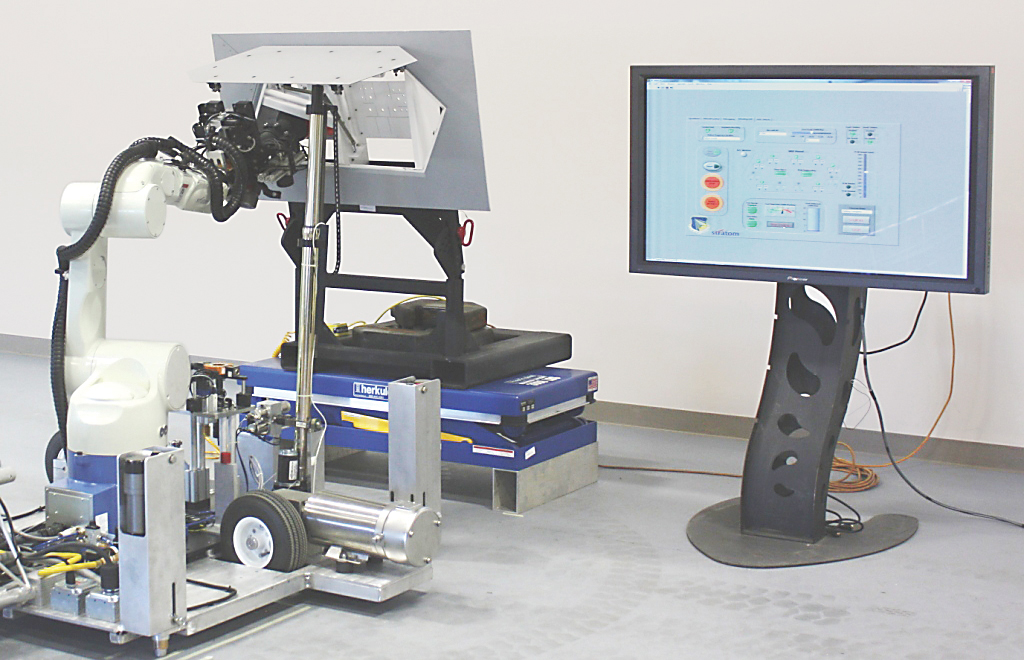
\includegraphics[width=0.6\textwidth]{figures/test_2010.jpeg}
    \caption{AFRL's Automated Aircraft Ground Refuelling system prototype robot (Photo Credit: AFRL/RXQ Robotics Group)}\label{fig:test-2010}
    \label{fig:test-2010}
\end{figure}

The Autonomous \& Robotic Remote Refuelling Point (AR3P) project, developed by
the U.S. Army, represents a pioneering initiative in unmanned refuelling
operations for rotary-wing aircraft. This project leverages advanced robotics,
including self-aligning mechanisms and articulated arms equipped with sensors,
to facilitate rapid and safe refuelling processes on non-contiguous
battlefields. The AR3P system minimises the time aircraft spend on the ground
and enhances safety by reducing soldier exposure at fueling stations. Initially
demonstrated in a Limited Initial Capabilities event, the AR3P aims to meet the
evolving range and endurance requirements of Army Aviation. The project
integrates existing technologies with novel systems designed in-house,
supported by commercial off-the-shelf components and additive manufacturing.
Currently, AR3P is progressing through its development phases, addressing
technical risks, and preparing for further testing and eventual deployment, as
shown in Figure~\ref{fig:test-2017} \cite{Ficken2017}.

\begin{figure}[H]
    \centering
    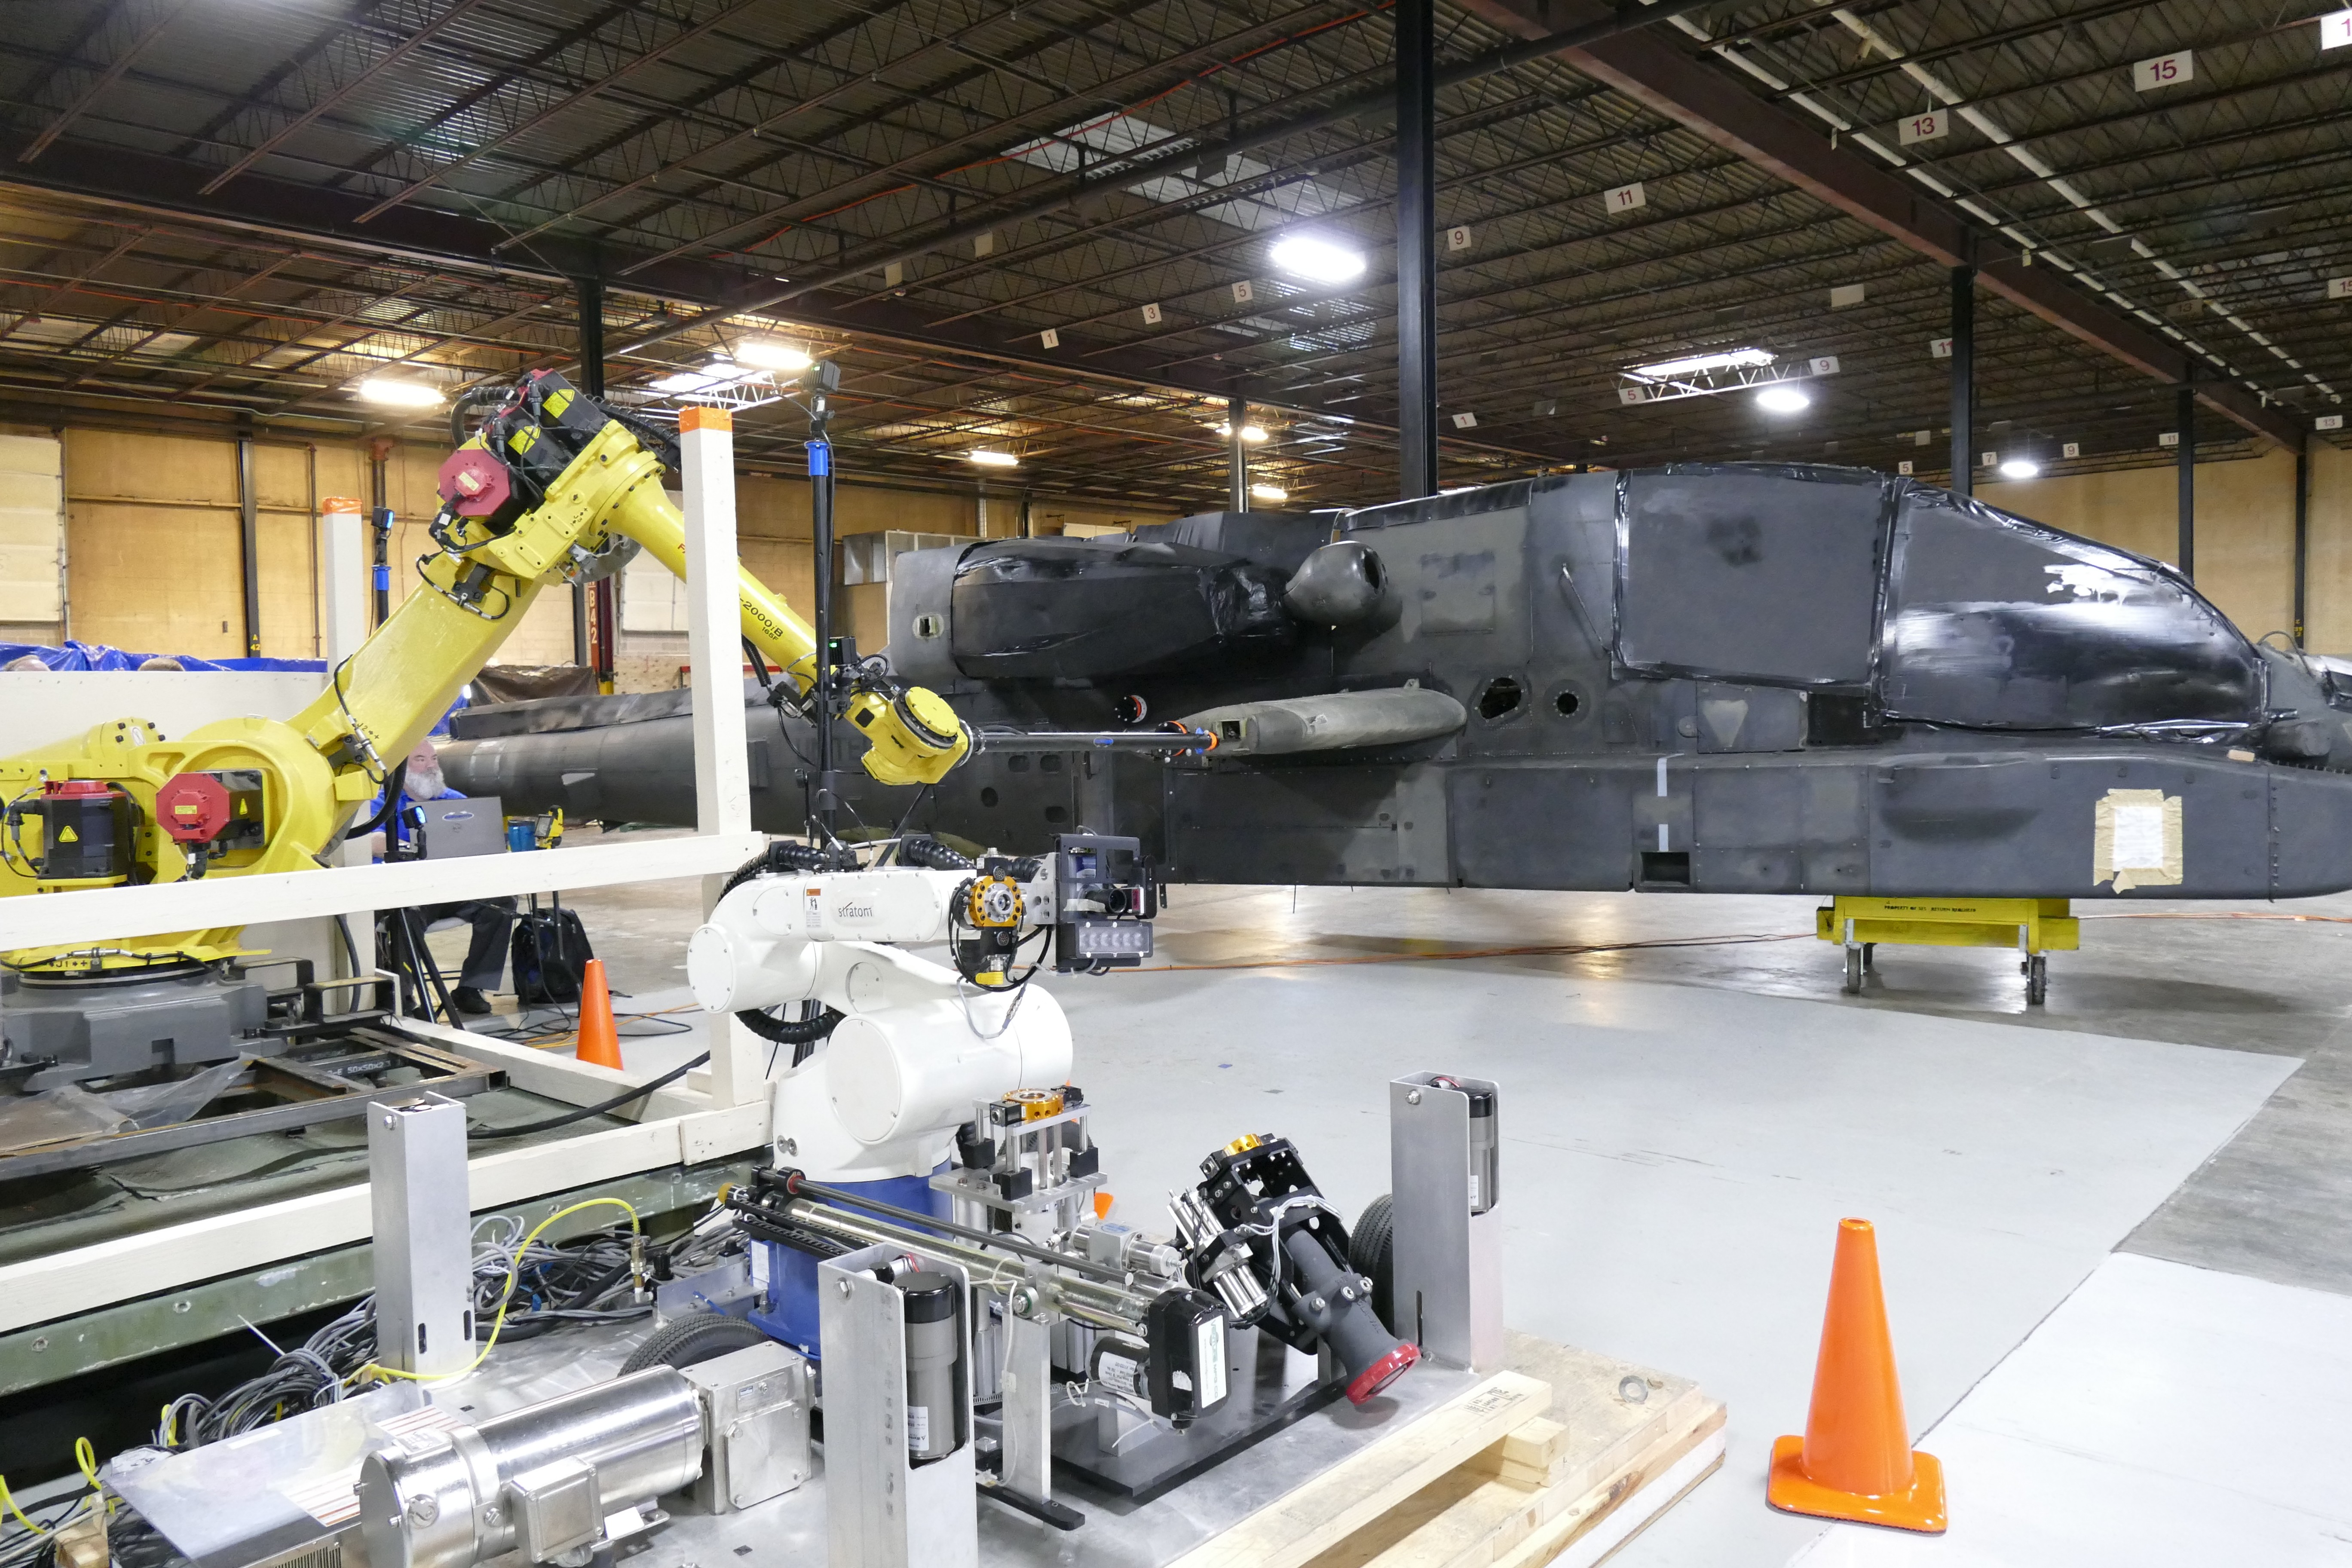
\includegraphics[width=0.5\textwidth]{figures/test_2017.jpg}
    \caption{AR3P Concept Development Prototype Robot (Photo Credit: U.S. Army)}\label{fig:test-2017}
\end{figure}

The AR3P project exemplifies the intersection of advanced robotics and
practical military applications, highlighting the potential of automated
systems to transform operational paradigms.
Figure~\ref{fig:automated-refuelling-systems} provides visual insights into the
capabilities of the AR3P system, by performing autonomous hot refuelling.
During this test, the robot is equipped with a LIDAR sensor and a camera to
detect the aircraft's refuelling port. In Figure~\ref{test-2020-2}, the AR3P
robot is seen approaching a detected aircraft, demonstrating its autonomous
navigation and alignment capabilities. In Figure~\ref{test-2020-3}, the AR3P
robot is shown engaging the aircraft refuelling port, emphasising its precision
and functionality in connecting to the aircraft’s fuel port. These images
illustrate the practical implementation of robotic technologies in enhancing
the safety, efficiency, and speed of refuelling operations, particularly in
challenging and hazardous environments \cite{AR3P2020}.

\begin{figure}[H]
    \centering
    \begin{subfigure}[b]{0.45\textwidth}
        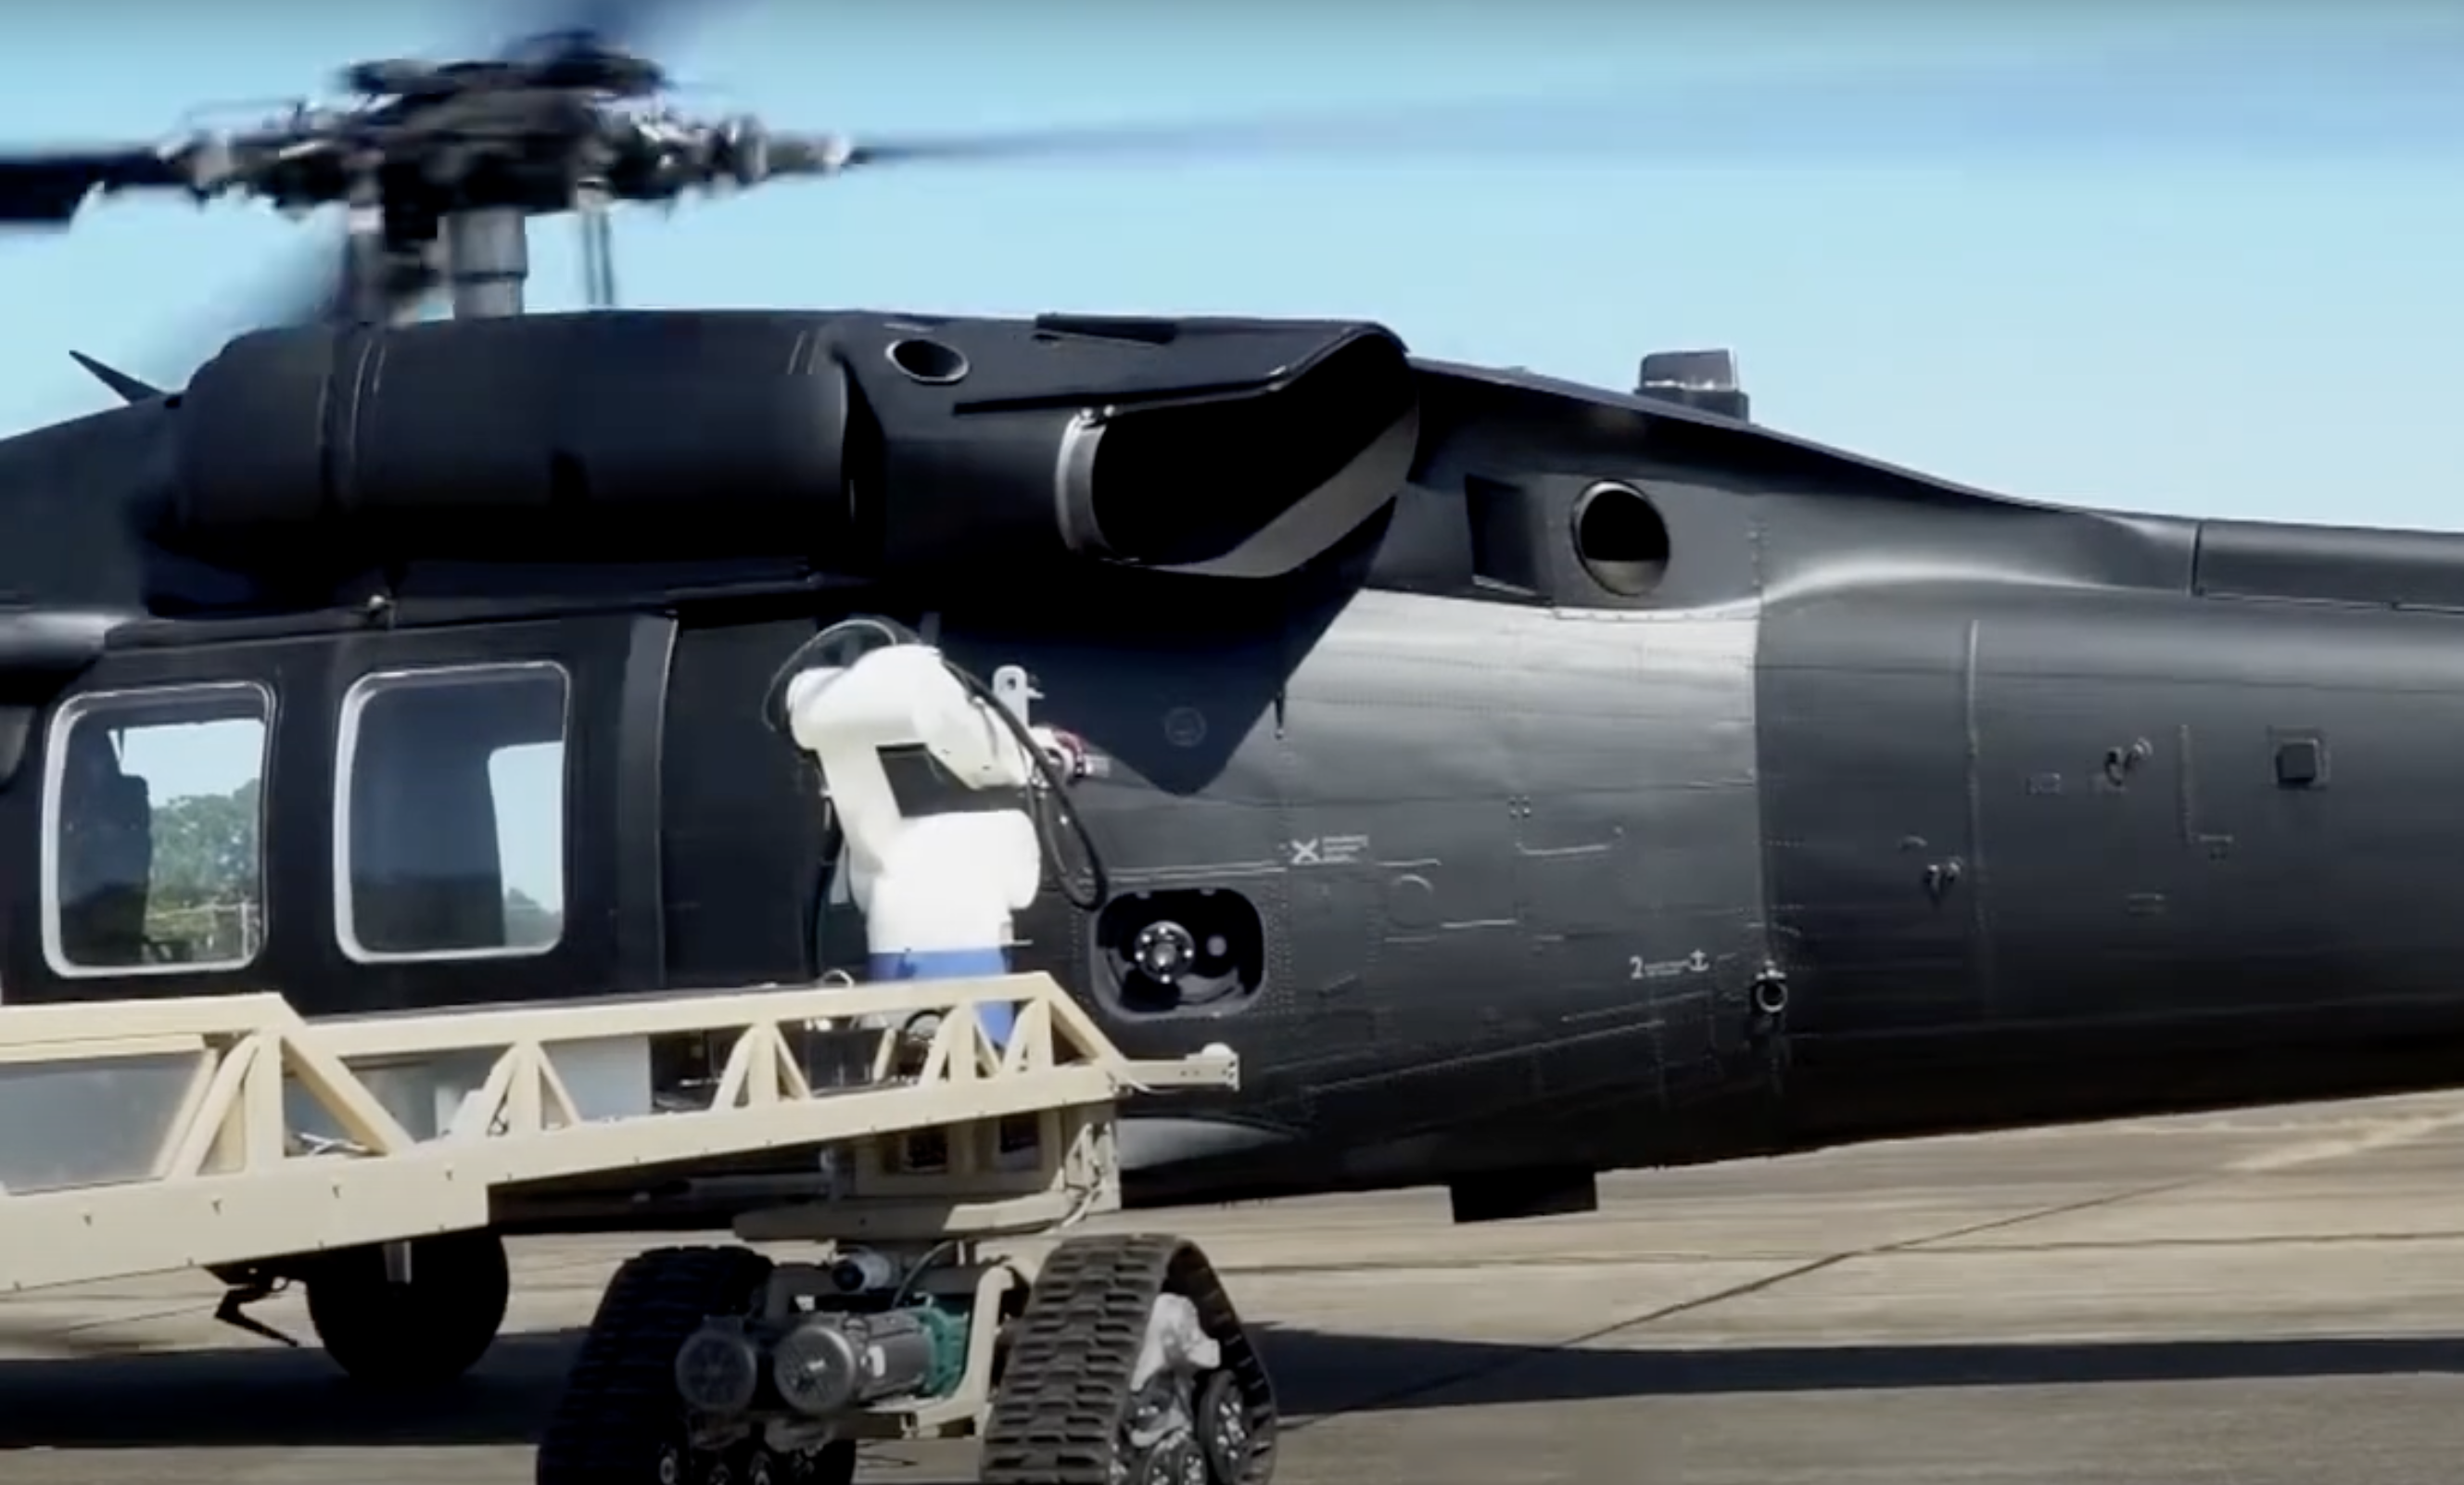
\includegraphics[height=0.68\textwidth, width=\textwidth]{figures/test_2020_2.png}
        \caption{AR3P Robot Approaching Detected Aircraft (Photo Credit: Stratom)}\label{test-2020-2}
    \end{subfigure}
    \hfill
    \begin{subfigure}[b]{0.45\textwidth}
        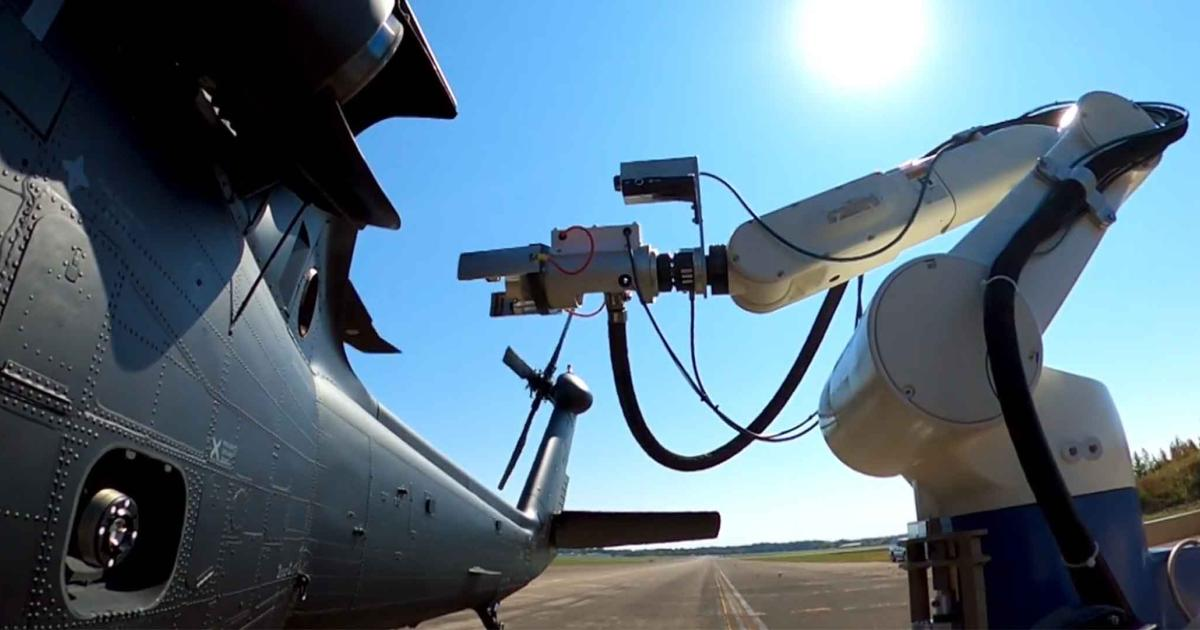
\includegraphics[height=0.68\textwidth, width=\textwidth]{figures/test_2020_3.jpg}
        \caption{AR3P Robot Engaging Aircraft Refuelling Port (Photo Credit: Stratom)}\label{test-2020-3}
    \end{subfigure}
    \caption{AR3P Robot Hot Refuelling Demonstration for S-70 Helicopter}\label{fig:automated-refuelling-systems}
\end{figure}

\newpage

Unfortunately, there is very little literature on existing AAGR systems, as
most research is carried out by the military and is classified. The most recent
papers cover Autonomous Aerial Refuelling (AAR) systems, which are used to
refuel unmanned aerial vehicles (UAVs) in mid-air. These systems are designed
to extend the flight time and range of UAVs by enabling them to refuel without
landing. AAR systems are particularly challenging due to the high speeds and
altitudes involved, as well as the need for precise measurement and tracking of
the relative position between the receiver aircraft and the tanker aircraft are
critical, particularly during the docking phase (see
figure~\ref{fig:aerial-refuelling})~\cite{AARBinocularVision,
    AARCNN}.~\citet{AAREKF} propose a robust solution that utilises monocular
vision combined with an extended Kalman filter (EKF) to address this challenge.
By implementing EKF, the system can provide reliable position estimations and
track the drogue within a specified region of interest (ROI), even in the
presence of disturbances such as air turbulence. As shown in
figure~\ref{fig:detection-system-aarekf}, this system initialises the state and
covariance matrices, predicts the drogue's position, updates the state based on
new measurements, and continuously refines the ROI for subsequent image
processing. This approach significantly reduces the processing time and
improves the detection frequency from 10 Hz to up to 30 Hz by focusing
computational resources on the predicted ROI. 

\begin{figure}[H]
    \centering
    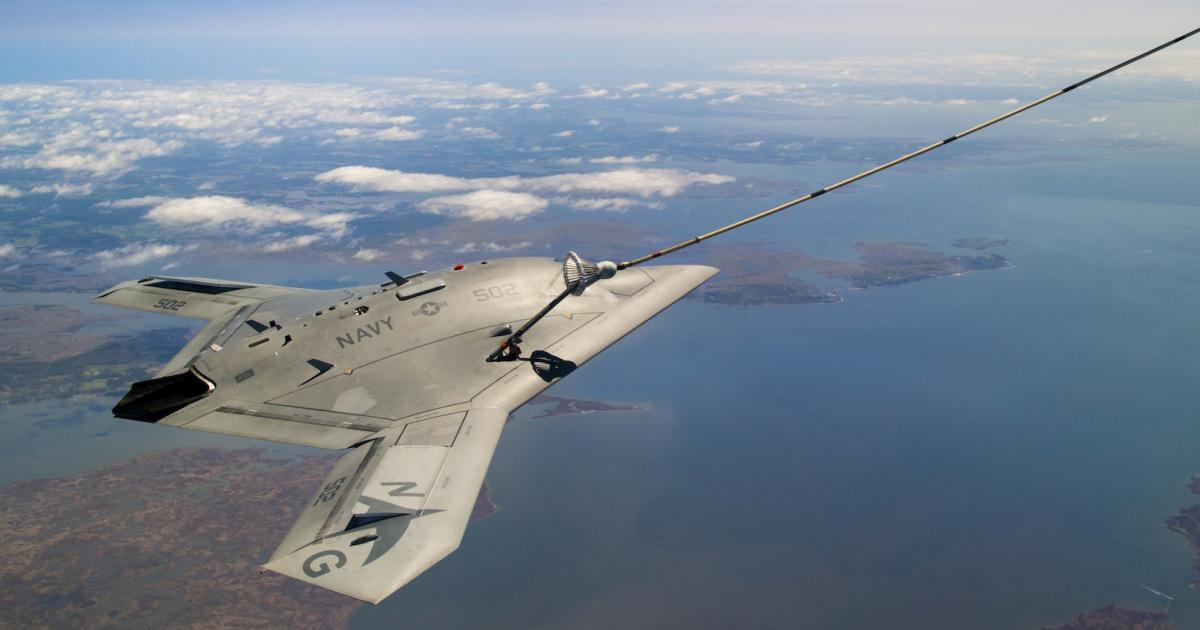
\includegraphics[width=0.4\textwidth]{figures/x-47brefueling.jpg}
    \caption{Autonomous Aerial Refuelling (AAR) of X-47B Unmanned Combat Air System Demonstrator (Photo Credit: U.S. Navy)}\label{fig:aerial-refuelling}
\end{figure}

\begin{figure}[H]
    \centering
    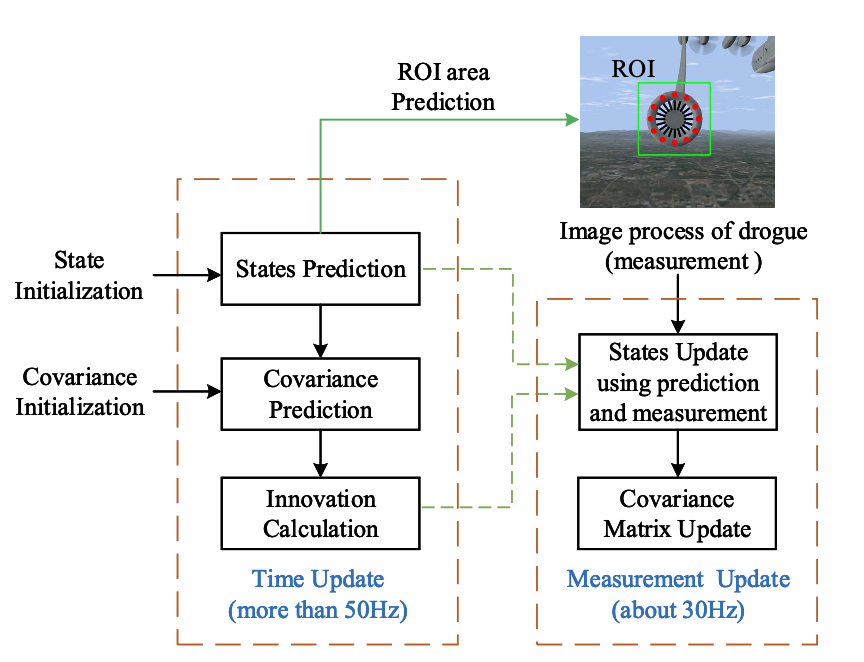
\includegraphics[width=0.6\textwidth]{figures/detection_system_AAREKF.png}
    \caption{Autonomous Air Refuelling Detection System with EKF. Source: \citet{AAREKF}}\label{fig:detection-system-aarekf}
\end{figure}

Recent advancements in autonomous ground refuelling have been driven by
improvements in computer vision and robotics.~\citet{AGRPoseEstimation}
presented the PosEst system, which combines 2D RGB images with 3D point cloud
data to enhance detection accuracy. This system uses a custom-trained
EfficientNet-B0 CNN for object detection and leverages the Kalman filter for
stable 3D pose estimation (see Figure~\ref{fig:agr-pose-kalman}). The PosEst
method employs a dual approach of high-precision detection and robust tracking.
By predicting and updating the object’s state in real-time, the Kalman filter
facilitates continuous and precise alignment of the fuel nozzle with the
refuelling adaptor, even in dynamic environments. This approach significantly
reduces the risks associated with manual refuelling and improves operational
efficiency and safety.

\begin{figure}[H]
    \centering
    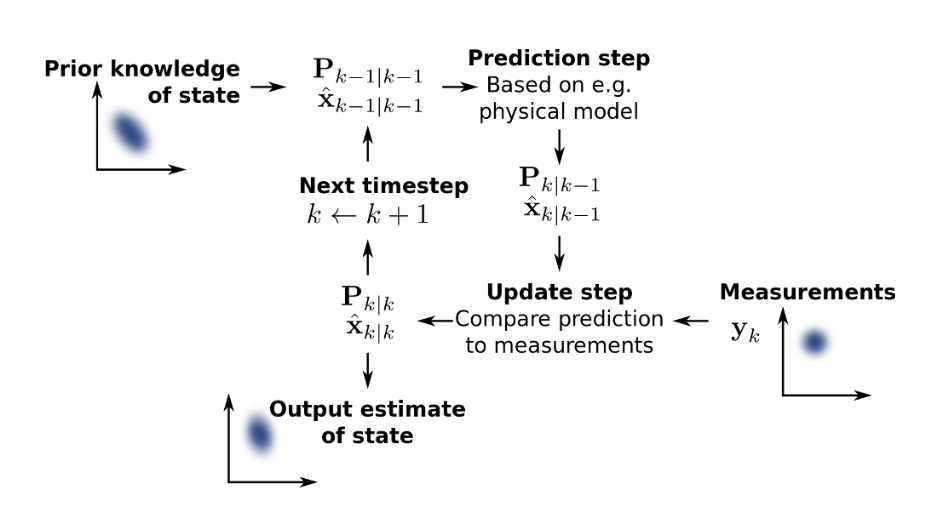
\includegraphics[width=0.65\textwidth]{figures/AGRPoseKalman.png}
    \caption{Kalman Filter Workflow for Pose Estimation in Autonomous Ground Refuelling. Source: \citet{AGRPoseEstimation}}\label{fig:agr-pose-kalman}
\end{figure}

One of the primary challenges in AAGR is the accurate detection and positioning
of the refuelling port under varying environmental conditions. Robust datasets
for scene recognition and machine learning applications have been developed to
address these challenges.~\citet{DatasetAGR} introduced a comprehensive dataset
for AAGR, addressing significant challenges such as variant illumination
conditions, different refuelling port types, and environmental obstructions.
The dataset comprises over 26,000 labeled images collected through image
crawling from 13 different databases, followed by augmentation to ensure
diversity (see Figure~\ref{fig:agr-dataset}). Additionally, recent innovations
have introduced hybrid datasets combining real and synthetic data for training
and validating systems \cite{HybridDatasetAGRV1}. This approach offers a wide
range of scenarios and conditions, improving the robustness and accuracy of
automated refuelling systems. The development of high-quality datasets is
pivotal in improving the robustness and reliability of AAGR systems.

\begin{figure}[H]
    \centering
    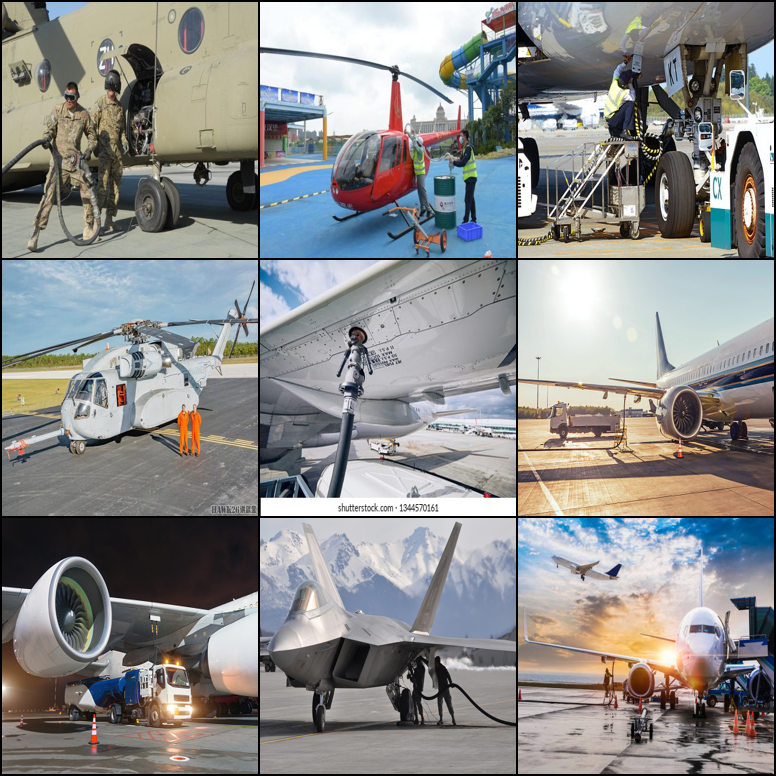
\includegraphics[width=0.38\textwidth]{figures/AGRDatasetGrid.png}
    \caption{AAGR Dataset Overview. Source: \citet{DatasetAGR}}\label{fig:agr-dataset}
\end{figure}

%%%%%%%%%%%%%%%%%%%%%%%%%%%%%%%%%%%%%%%%%%%%%%%%%%%%%%%%%%%%%%%%%%%%%%%%%%%%%%%%

\newpage
\section{Object Detection and Tracking in Computer Vision}
In Computer Vision, Object Detection refers to the identification and location
of individual objects within an image, providing both spatial information
(bounding boxes) and confidence scores, which represent the probability that
each detected object belongs to the predicted
class~\cite{huggingface2023objectdetection}. For example, in the following
image, there are five detections, including one `ball' with a confidence level
of 98\% and four `people' with confidence levels of 98\%, 95\%, 97\% and 97\%.
Evaluating Object Detection models involves several key metrics to measure
their performance. One common metric is Intersection over Union (IoU), which
measures the overlap between a predicted bounding box and a ground-truth
bounding box, as shown in Figure~\ref{fig:iou-metric}.

\begin{figure}[H]
    \centering
    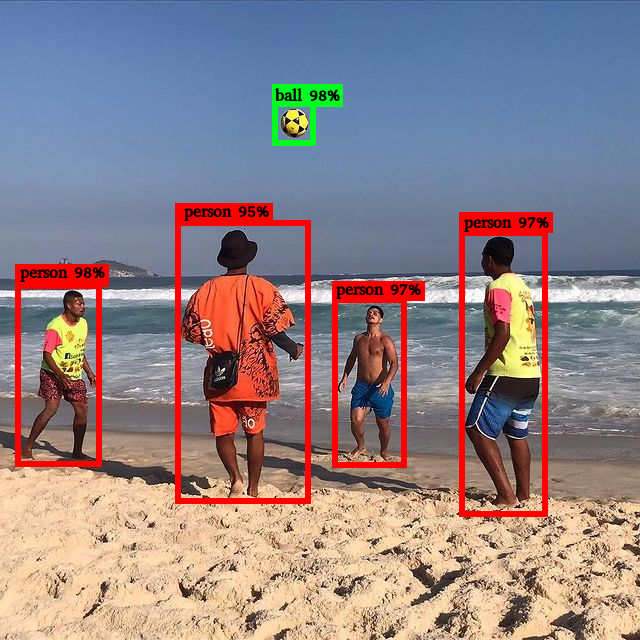
\includegraphics[width=0.3\textwidth]{figures/intro_object_detection.png}
    \caption{Example of outputs from an object detector~\cite{huggingface2023objectdetection}.}\label{fig:object-detection}
\end{figure}

\begin{figure}[H]
    \centering
    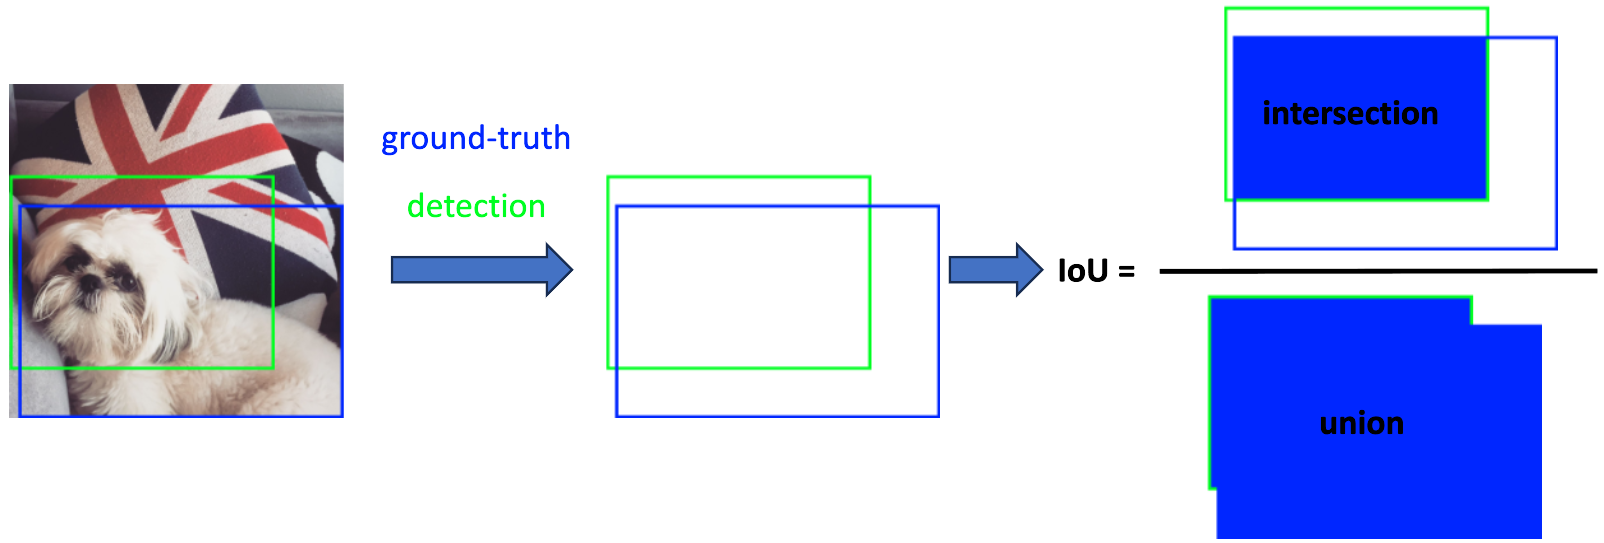
\includegraphics[width=0.8\textwidth]{figures/iou.png}
    \caption{Intersection over Union (IoU) between a detection (in green) and ground-truth (in blue).~\cite{huggingface2023objectdetection}}\label{fig:iou-metric}
\end{figure}

Over the last few decades, Object Detection models based on Deep Learning have
enjoyed remarkable success. These models fall into two main categories:
two-stage detectors and single-stage detectors. On the one hand, two-stage
detectors, such as R-CNN~\cite{DBLP:journals/corr/GirshickDDM13}, Fast
R-CNN~\cite{DBLP:journals/corr/Girshick15}, Faster R-CNN~\cite{Ren2017} and
R-FCN~\cite{DBLP:journals/corr/DaiLHS16}, first generate region proposals and
then refine these proposals into precise anchor boxes. While these models excel
in detection accuracy, they typically suffer from large model sizes and slower
detection speeds~\cite{SurveyDLOD, ODNetworkUAVCNNTransformer}. On the other
hand, single-stage detectors, including the SSD (Single Shot Multibox
Detector)~\cite{DBLP:journals/corr/LiuAESR15}, YOLO (You Only Look Once)
series~\cite{DBLP:journals/corr/RedmonDGF15, DBLP:journals/corr/RedmonF16,
    DBLP:journals/corr/abs-2004-10934, chen2023yoloms,
    DBLP:journals/corr/abs-2107-08430, YOLOv5Release, li2023yolov6, YOLOv8,
    wang2024yolov9, xu2022ppyoloe, wang2023goldyolo, xu2023damoyolo,
    wang2024yolov10}, and RetinaNet~\cite{lin2018focal} directly predict object
locations and categories in a single network pass. These models are known for
their high detection speeds but sometimes compromise accuracy~\cite{SurveyDLOD,
    ODNetworkUAVCNNTransformer}.

\begin{figure}[H]
    \centering
    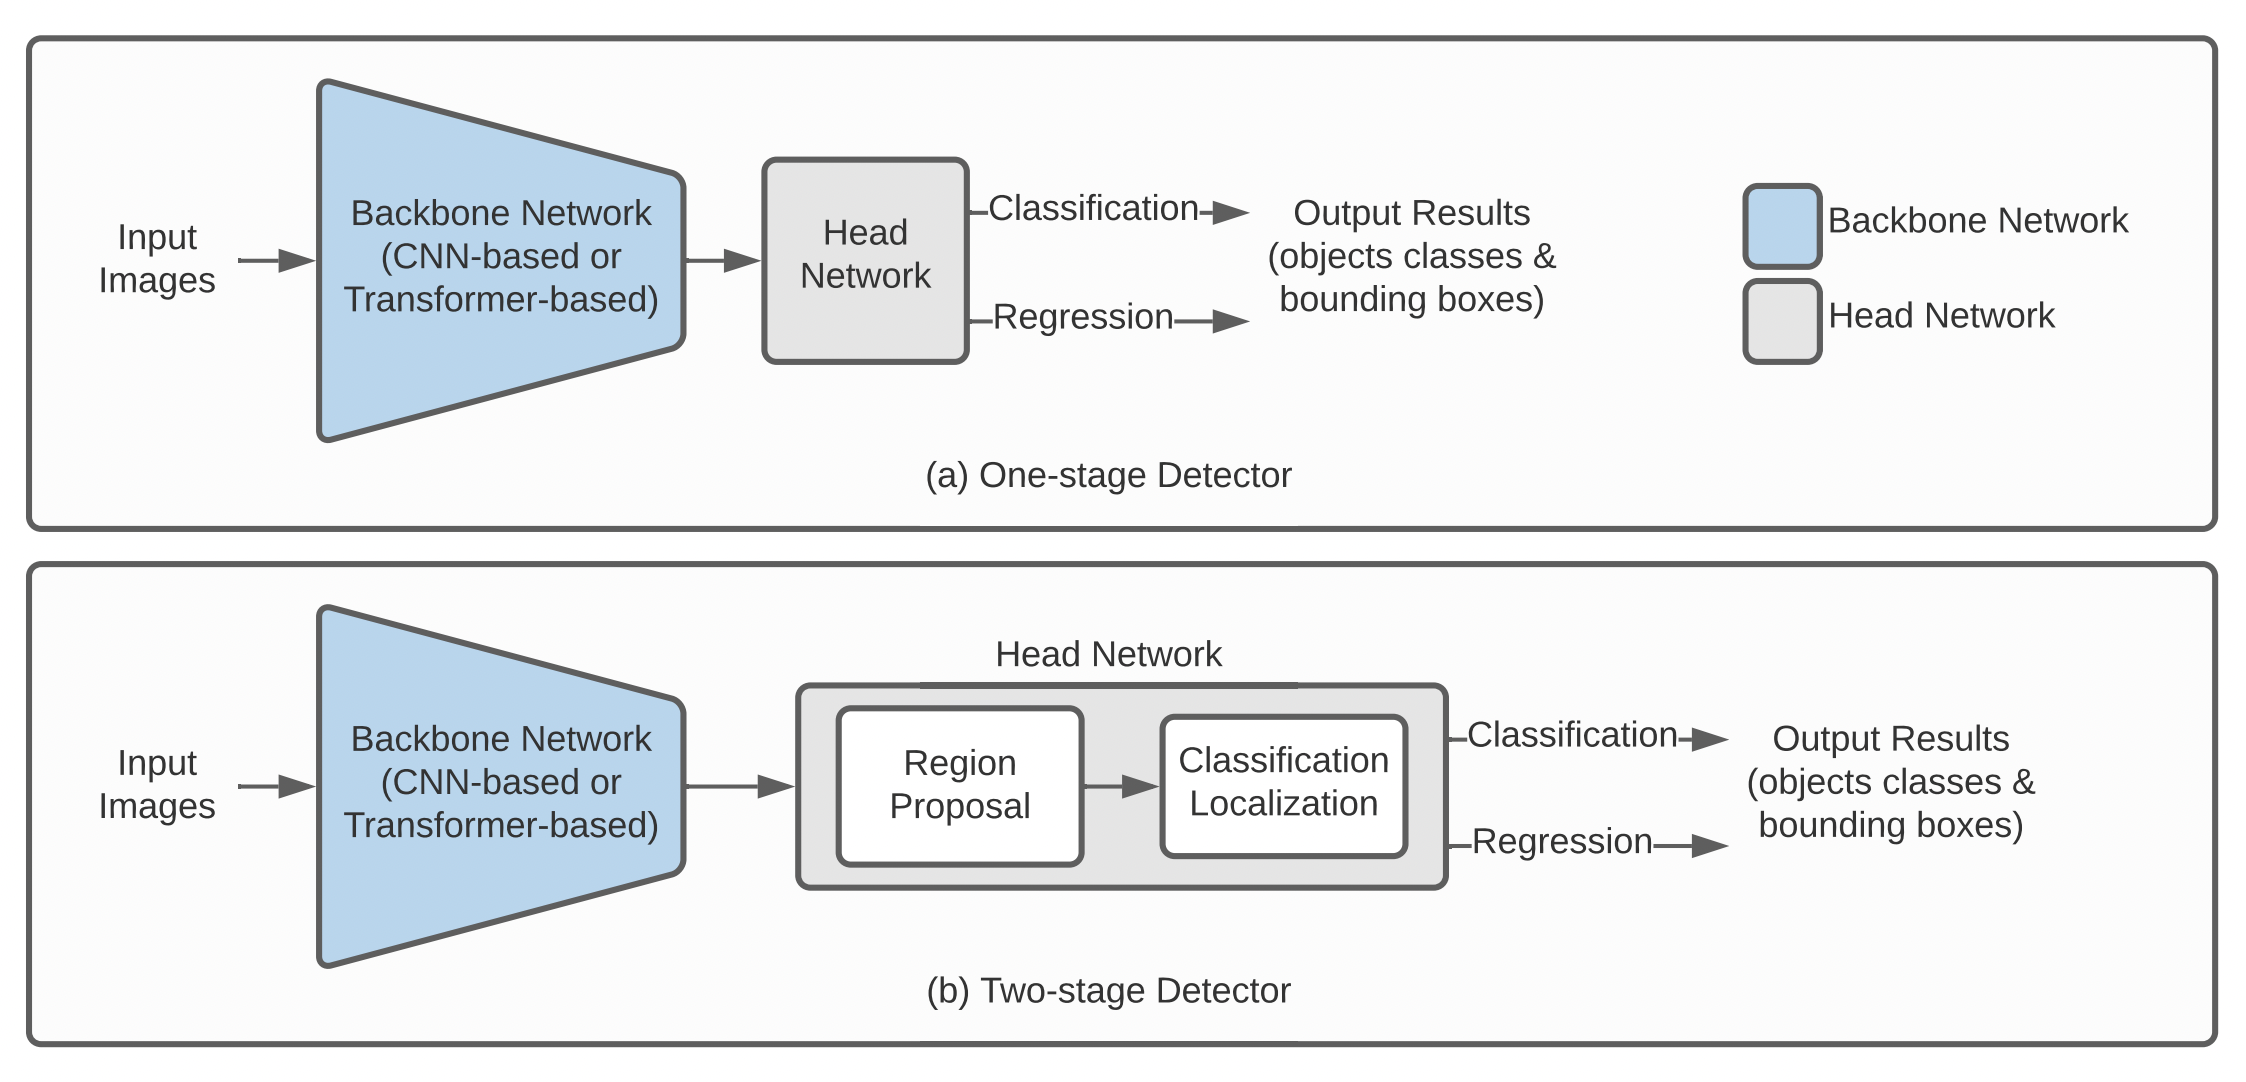
\includegraphics[width=0.8\textwidth]{figures/one-stage_two-stage_OD.png}
    \caption{Basic deep learning-based one-stage vs two-stage object detection model architectures~\cite{SurveyDLOD}.}\label{fig:two-stage-vs-single-stage}
\end{figure}

YOLOv10, the latest iteration in the YOLO series, marks a significant leap
forward in real-time object detection with the introduction of NMS-free
training. Traditionally, single-stage detectors relied on Non-Maximum
Suppression (NMS) during post-processing to eliminate redundant predictions, as
illustrated in Figure~\ref{fig:nms}. However, this process can sometimes be
overly aggressive, risking the loss of valuable predictions or failing to
remove all duplicates effectively, which also adds to computational costs
during both training and inference~\cite{LearnOpenCVYOLOv10}.

\begin{figure}[H]
    \centering
    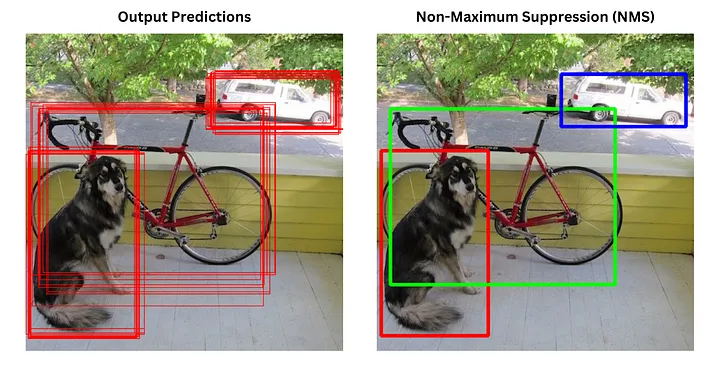
\includegraphics[width=0.5\textwidth]{figures/NMS.png}
    \caption{Non-Maximum Suppression (NMS) in Object Detection~\cite{LearnOpenCVYOLOv10}.}\label{fig:nms}
\end{figure}

\noindent YOLOv10 overcomes these limitations by implementing a consistent dual
assignments strategy that facilitates NMS-free training. This strategy
leverages both one-to-many and one-to-one label assignments during training,
providing the model with rich supervision while enabling efficient end-to-end
deployment. During inference, the one-to-one assignment head is employed, which
eliminates the need for NMS and significantly reduces inference time. As
depicted in Figure~\ref{fig:yolov10}, the one-to-many head assigns multiple
labels to each anchor box, enriching the model’s supervision, while the
one-to-one head refines these predictions by assigning a single label to each
anchor box, ensuring precise and efficient detection~\cite{wang2024yolov10}.

\begin{figure}[H]
    \centering
    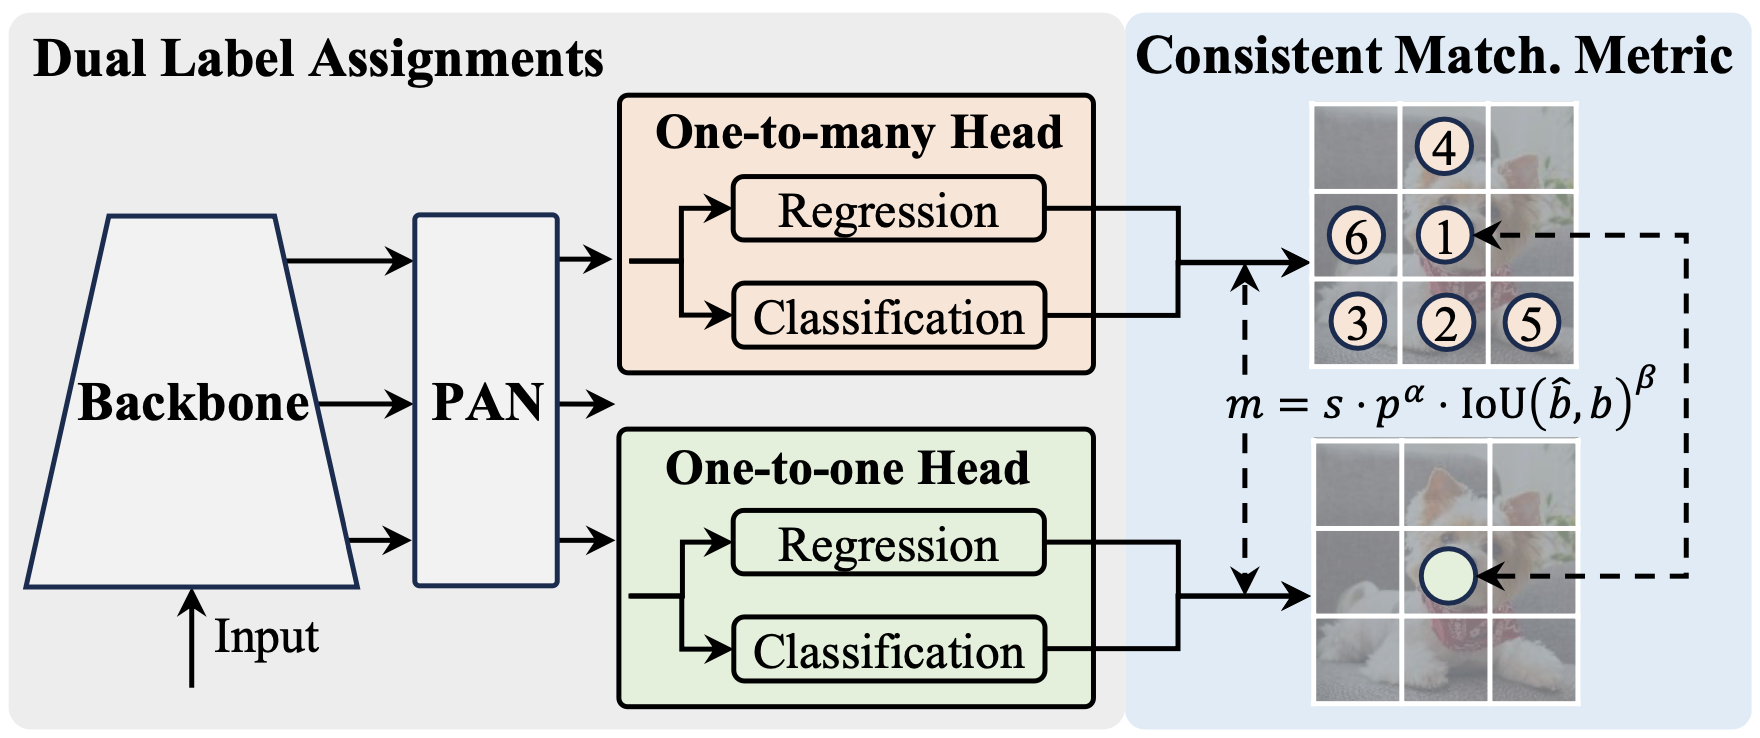
\includegraphics[width=0.5\textwidth]{figures/YOLOV10.png}
    \caption{YOLOv10 Model Workflow~\cite{wang2024yolov10}}\label{fig:yolov10}
\end{figure}

\noindent In addition, YOLOv10 adopts a holistic efficiency-accuracy driven design that
optimises the model’s architecture across various dimensions. The
classification head has been redesigned to be more lightweight, reducing
computational overhead while maintaining accuracy. The spatial-channel
decoupled downsampling technique separates spatial reduction and channel
increase operations, which lowers computational costs and reduces the parameter
count. Furthermore, the rank-guided block design minimises redundancy within
the model by adapting the complexity of different stages based on their
intrinsic rank values, ensuring optimal capacity-efficiency trade-offs. YOLOv10
also introduces large-kernel (see figure~\ref{fig:large-kernel-yolov10})
convolutions selectively in the deeper stages of the network to increase the
receptive field, allowing the model to capture more contextual information
without a significant increase in computational cost. Moreover, YOLOv10
incorporates a partial self-attention (PSA) mechanism, which integrates the
benefits of global context modelling while maintaining a lightweight
architecture. This careful balance of efficiency and accuracy enables YOLOv10
to deliver state-of-the-art
performance~\cite{wang2024yolov10,LearnOpenCVYOLOv10}.

\begin{figure}[H]
    \centering
    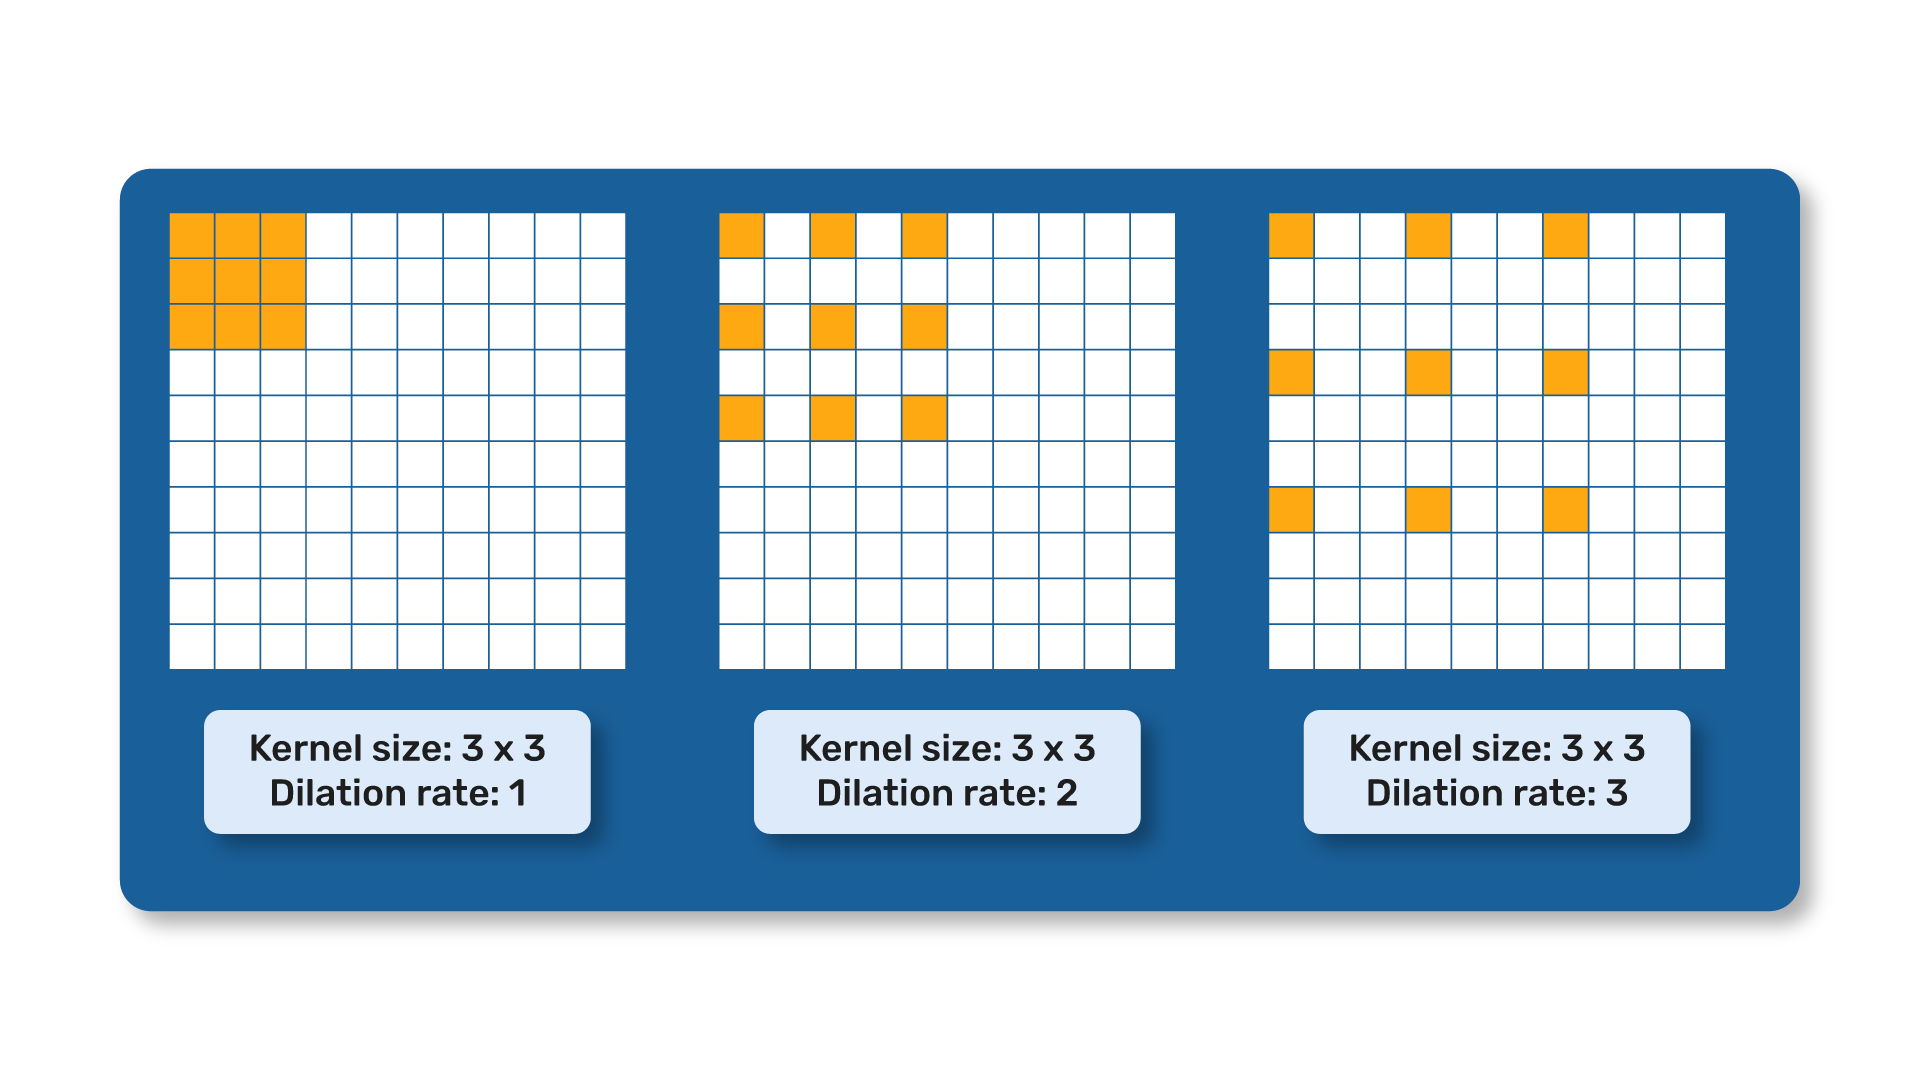
\includegraphics[width=0.5\textwidth]{figures/KernelYOLOv10.png}
    \caption{Large-Kernel Convolution in YOLOv10~\cite{LearnOpenCVYOLOv10}}\label{fig:large-kernel-yolov10}
\end{figure}

\noindent As shown in Table~\ref{tab:yolov10-benchmarks}, extensive testing on standard
benchmarks, such as COCO, demonstrates YOLOv10’s superior performance in both
speed and accuracy. For example, YOLOv10-S is 1.8 times faster than RT-DETR-R18
while also using fewer parameters. Similarly, YOLOv10-B achieves a 46\%
reduction in latency compared to YOLOv9-C without compromising performance.
These results underscore YOLOv10’s effectiveness as a real-time end-to-end
object detection model, making it well-suited for applications requiring both
high speed and accuracy.

\begin{table}[H]
    \centering
    \caption{Performance Comparison of YOLO Models with State-of-the-Art Techniques~\cite{wang2024yolov10}.}
    \begin{adjustbox}{max width=0.75\textwidth}
        \begin{tabular}{lccccc}
            \toprule
            \textbf{Model}     & \textbf{Params (M)} & \textbf{FLOPs (G)} & \textbf{AP\textsubscript{val} (\%)} & \textbf{Latency (ms)} \\
            \midrule
            YOLOv6-3.0-N       & 4.7                 & 11.4               & 37.0                                & 2.69                  \\
            Gold-YOLO-N        & 5.6                 & 12.1               & 39.6                                & 2.92                  \\
            YOLOv8-N           & 3.2                 & 8.7                & 37.3                                & 6.16                  \\
            \textbf{YOLOv10-N} & \textbf{2.3}        & \textbf{6.7}       & \textbf{39.5}                       & \textbf{1.84}         \\  
            \midrule
            YOLOv6-3.0-S       & 18.5                & 45.3               & 44.3                                & 3.42                  \\  
            Gold-YOLO-S        & 21.5                & 46.0               & 45.4                                & 3.82                  \\  
            YOLO-MS-XS         & 4.5                 & 17.4               & 43.4                                & 8.23                  \\  
            YOLO-MS-S          & 8.1                 & 31.2               & 46.2                                & 10.12                 \\  
            YOLOv8-S           & 11.2                & 28.6               & 44.9                                & 7.07                  \\  
            YOLOv9-S           & 7.1                 & 26.4               & 46.7                                & -                     \\  
            RT-DETR-R18        & 20.0                & 60.0               & 46.5                                & 4.58                  \\  
            \textbf{YOLOv10-S} & \textbf{7.2}        & \textbf{21.6}      & \textbf{46.8}                       & \textbf{2.49}         \\  
            \midrule
            YOLOv6-3.0-M       & 34.9                & 85.8               & 49.1                                & 5.63                  \\  
            Gold-YOLO-M        & 41.3                & 87.5               & 49.8                                & 6.38                  \\  
            YOLO-MS            & 22.2                & 80.2               & 51.0                                & 12.41                 \\  
            YOLOv8-M           & 25.9                & 78.9               & 50.6                                & 9.50                  \\  
            YOLOv9-M           & 20.0                & 76.3               & 51.1                                & -                     \\  
            RT-DETR-R34        & 31.0                & 92.0               & 48.9                                & 6.32                  \\  
            RT-DETR-R50m       & 36.0                & 100.0              & 51.3                                & 6.90                  \\  
            \textbf{YOLOv10-M} & \textbf{15.4}       & \textbf{59.1}      & \textbf{51.3}                       & \textbf{4.74}         \\  
            \bottomrule
        \end{tabular}
    \end{adjustbox}
    \label{tab:yolov10-benchmarks}
\end{table}

In addition to Object Detection, Object Tracking is another critical task in
Computer Vision, involving the continuous monitoring of objects across video
frames. Object Tracking methods can be broadly classified into two categories:
\textbf{Generative Trackers} and \textbf{Discriminative
    Trackers}~\cite{SurveyVisualOT}. Generative trackers are capable of handling
challenging scenarios such as occlusion and large-scale variation through
particle sampling strategies, often integrated with various appearance models,
including sparse representation and energy of motion. Discriminative trackers,
by contrast, build robust classifiers using hand-crafted or deep
features~\cite{SurveyVisualOT}. The combination of generative and
discriminative approaches, as well as the integration of deep learning
techniques such as fully revolutionary networks and Transformer models, has led
to significant improvements in object detection
performance~\cite{OverviewCorrelationAlgoOT, SuveyAdvancesSingleOTMethods,
    SurveyModernODModels}. In addition, the speed and computational requirements of
these algorithms are critical factors influencing their practical
applicability~\cite{SuveyAdvancesSingleOTMethods, SurveyModernODModels,
    SurveyTransformersSingleOT}. Advanced techniques in object tracking leverage
both generative and discriminative models to amplify tracking efficacy. The
utilisation of deep trackers has evidenced superior results on public tracking
datasets, attributed to their potent feature extractors, accurate bounding box
regressors, and discriminative classifiers~\cite{SurveyTransformersSingleOT}.
Techniques such as deformable convolution and Transformer models extend
traditional convolution or correlation methodologies to execute global feature
matching, thereby enhancing tracking accuracy. The incorporation of contextual
or knowledge information can substantially elevate performance, with
methodologies like Particle Filtering, also recognised as Sequential Monte
Carlo (SMC) methods, framed as problems of Bayesian inference in state
space~\cite{SurveySmallObjectDetection, SmallObjectDetectionPositonPrediction}.
The extended Kalman Filtering (EKF) is another advanced technique that has been
employed to improve tracking accuracy by predicting the current status through
the previous status and modifying the prediction result based on observation
information~\cite{SuveyAdvancesSingleOTMethods, SurveyModernODModels}. Despite
these advancements, the integration of these methods in a complementary manner
remains an open research area with substantial potential for advancing the
field~\cite{OverviewCorrelationAlgoOT, SuveyAdvancesSingleOTMethods}.

\newpage
\section{Deep Learning for Spacio-Temporal Prediction}
Time series prediction involves processing sequential data to predict future
events or values. Various deep learning models have been applied to this task,
requiring several preparatory steps such as collecting data, designating
attribute types, dealing with inconsistencies and storing datasets. These
datasets are usually classified into units of time such as seconds, minutes and
hours, allowing the construction of metadata for machine
learning~\cite{FFPSpaceSystemVehicles}.

\subsection*{State-of-the-Art Sequence Models}

The prediction of future object locations has been a critical focus of
research, particularly in autonomous driving and surveillance applications.
Early approaches to this problem primarily utilised Recurrent Neural Networks
(RNNs), which include Long Short-Term Memory networks (LSTMs) and Gated
Recurrent Units (GRUs)~\cite{Alemany2019, Bemporad2023,
    PredictionHeadMovement360Degrees}. These models employ an encoder-decoder
architecture to encode sequences of past observations and decode future
locations. The encoder processes the input sequence to capture temporal
dependencies, while the decoder predicts the future sequence based on the
encoded information. RNNs, especially LSTMs and GRUs, have shown significant
potential in sequence prediction tasks due to their ability to model long-term
dependencies~\cite{CubicLSTMsVideoPrediction, ConvLSTM,
    DBLP:journals/corr/SrivastavaMS15}. However, these models often suffer from
performance degradation over time, primarily because they recursively predict
future bounding boxes based on the previous outputs, which can lead to error
accumulation~\cite{FusionGRU}. To address these limitations, early models
incorporated additional contextual inputs, such as environmental data and
semantic actions, to improve prediction accuracy. For example,
\citet{Alahi2016} introduced the Social-LSTM model, which accounts for the
interactions between pedestrians, using a social pooling mechanism to enhance
global context understanding and improve trajectory predictions. As depicted in
Figure~\ref{fig:lstm-rnn-gru}, the key differences between RNN, LSTM, and GRU
models lie in their internal architectures and mechanisms for handling
information flow over time. LSTMs and GRUs are designed to mitigate the
vanishing gradient problem commonly associated with standard RNNs by
incorporating gating mechanisms. These gates control the flow of information,
allowing the model to retain or forget certain information as needed, thereby
improving its ability to capture long-term dependencies.

\begin{figure}[H]
    \centering
    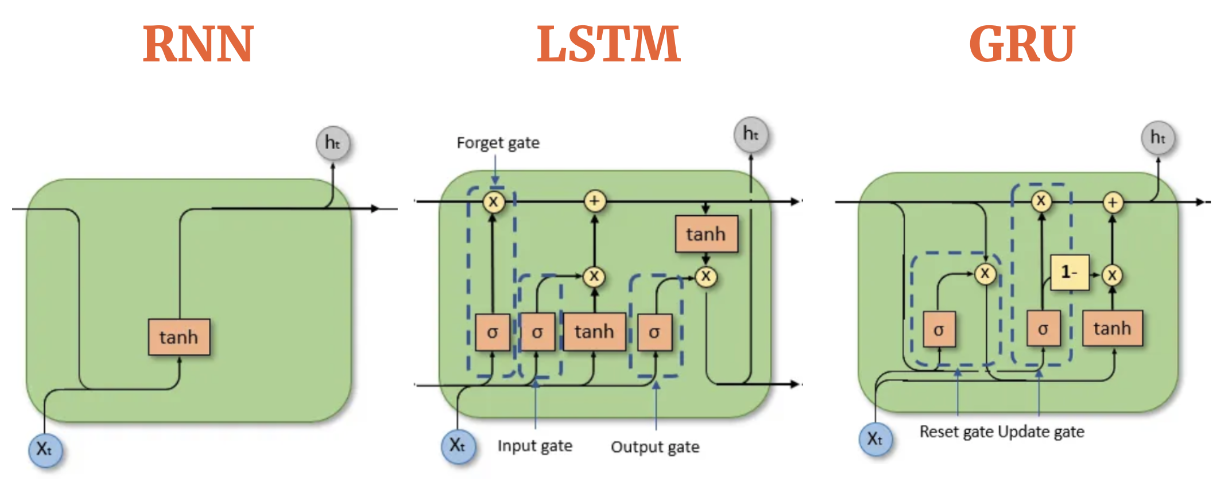
\includegraphics[width=1\textwidth]{figures/lstm-rnn-gru.png}
    \caption{Comparing different Sequence models: RNN, LSTM, and GRU. Source: Colah's blog. Compiled by AIML.com}\label{fig:lstm-rnn-gru}
\end{figure}

\newpage
\subsection*{Use of LSTMs and GRUs in Sequence Prediction}
\subsubsection*{Spatio-Temporal Encoder-Decoder (STED) Model}

The STED model was introduced by~\citet{MultipleObjectForecasting} as a novel
approach for multiple object forecasting (MOF), particularly in predicting the
future bounding boxes of tracked objects from video sequences. This model is
designed to handle the challenges of object forecasting in diverse
environments, leveraging both visual and temporal features to predict
object-motion and ego-motion effectively. As shown in Figure~\ref{fig:sted},
the STED model consists of three main components: a bounding box feature
encoder, an optical flow feature encoder, and a decoder. The \textit{Bounding
    Box Feature Encoder} utilises a Gated Recurrent Unit (GRU) to extract temporal
features from past object bounding boxes, which include coordinates $(x, y)$,
dimensions $(w, h)$, and velocity changes $(\Delta x, \Delta y, \Delta w,
    \Delta h)$ over a window of 30 frames, representing 1 second of observation.
Simultaneously, the \textit{Optical Flow Feature Encoder} captures motion
features directly from optical flow, using a Convolutional Neural Network (CNN)
to process a stack of 10 frames sampled uniformly from the past 1 second of
video data. The combination of these features provides a comprehensive
understanding of both the object's movement and the camera's movement
(ego-motion). The \textit{Decoder} then takes the concatenated feature vector
from the encoders and predicts the future bounding box coordinates for the next
60 frames (2 seconds prediction window). The GRU-based decoder generates
bounding box predictions iteratively, using the encoded feature vector and the
internal hidden state to output changes in bounding box velocity and dimensions
over time.

\begin{figure}[H]
    \centering
    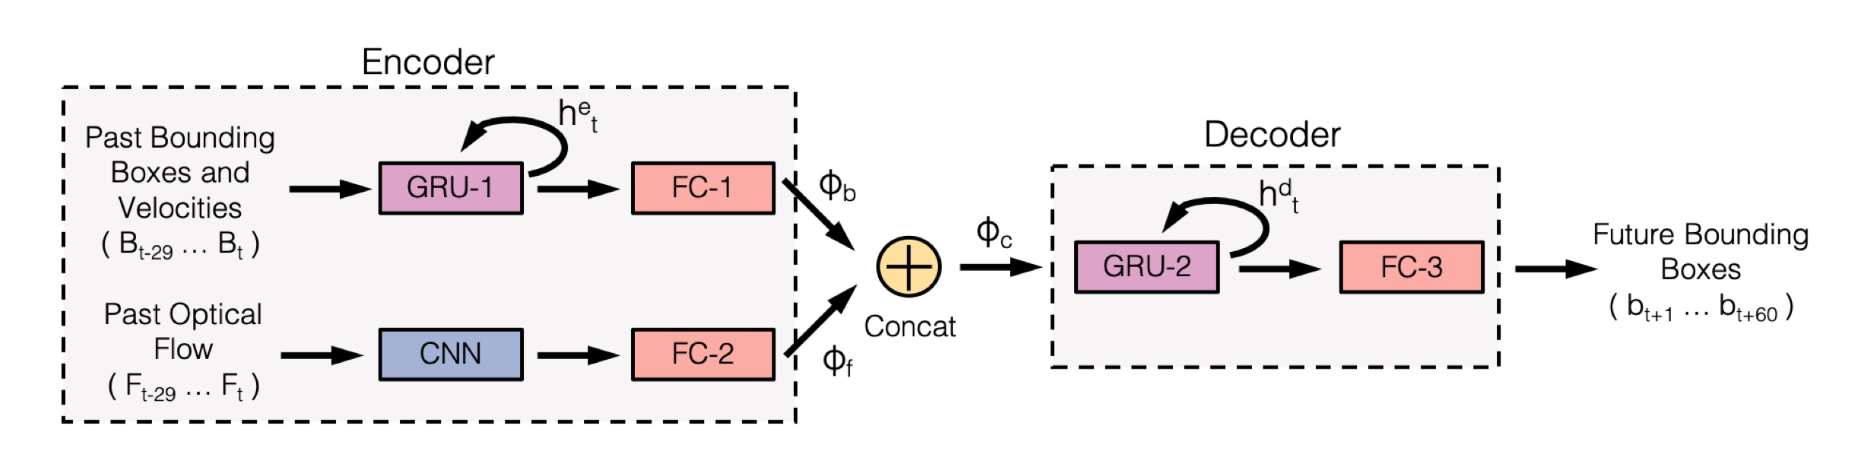
\includegraphics[width=1\textwidth]{figures/STED.png}
    \caption{STED Model Architecture. Source:~\citet{MultipleObjectForecasting}}\label{fig:sted}
\end{figure}

The STED architecture is specifically designed to address the complexities of
predicting future object positions in video sequences, particularly under
conditions of non-linear object motion and varying scales due to camera
movement. By combining temporal features from bounding boxes with motion
information from optical flow, the model effectively captures both the dynamic
behaviour of the objects and the impact of the camera's motion on the observed
scene. The STED model was evaluated on the Citywalks
dataset~\cite{MultipleObjectForecasting}, a diverse dataset designed to test
the model's ability to predict future object locations across different
environments. The performance of STED was compared with several baseline
models, as summarised in Table~\ref{tab:sted-results}. Metrics include Average
Displacement Error (ADE), Final Displacement Error (FDE), Average
Intersection-over-Union (AIoU), and Final Intersection-over-Union (FIoU). The
model was evaluated using 1 second of input frames to predict 2 seconds of
future frames.
\begin{table}[H]
    \centering
    \caption{Comparison of the performance of STED with baseline models on the Citywalks dataset. }
    \begin{adjustbox}{max width=\textwidth}
        \begin{tabular}{lcccc}
            \toprule
            \textbf{Model}                         & \textbf{ADE (pixels)} & \textbf{FDE (pixels)} & \textbf{AIoU (\%)} & \textbf{FIoU (\%)} \\ 
            \midrule
            CV-CS~\cite{MultipleObjectForecasting} & 31.6                  & 57.6                  & 46.0               & 21.3               \\
            LKF~\cite{MultipleObjectForecasting}   & 32.9                  & 59.0                  & 43.9               & 20.1               \\
            STED~\cite{MultipleObjectForecasting}  & \textbf{26.0}         & \textbf{46.9}         & \textbf{51.8}      & \textbf{27.5}      \\
            \bottomrule
        \end{tabular}
    \end{adjustbox}
    \label{tab:sted-results}
\end{table}

\noindent The STED model achieved an Average Displacement Error (ADE) of 26.0 pixels and
a Final Displacement Error (FDE) of 46.9 pixels, with an Average Intersection
Over Union (AIoU) of 51.8\% and a Final Intersection Over Union (FIoU) of
27.5\%. These results indicate that STED outperforms existing models in both
displacement and intersection-over-union metrics, making it a robust solution
for forecasting future object locations in challenging video sequences.

\subsubsection*{Position-Velocity Long Short-Term Memory (PV-LSTM) Model}

The PV-LSTM model was developed by~\citet{DBLP:journals/corr/abs-2010-10270} to
predict pedestrian intentions and future bounding box positions, a crucial task
for enhancing the safety of autonomous driving systems. The architecture of
this model is illustrated in Figure~\ref{fig:pv-lstm}. The model utilises a
sequence-to-sequence LSTM architecture that processes both spatial and temporal
information effectively. To do that, it processes input sequences of observed
bounding boxes $(x, y, w, h)$ and their velocity changes $(\Delta x, \Delta y,
    \Delta w, \Delta h)$ over a window of 30 frames, representing 1 second of
observation. These inputs are encoded through two encoders: the
\textit{Bounding Box Position Encoder} and the \textit{Bounding Box Velocity
    Encoder}. The encoded features are then concatenated and passed to two
decoders: the \textit{Velocity Decoder}, which predicts future bounding box
velocities, and the \textit{Intention Decoder}, which predicts pedestrian
crossing intentions over the next 60 frames (2 seconds prediction window). The
PV-LSTM model’s architecture is designed to capture the dynamic and complex
nature of pedestrian behaviour, which is crucial for real-time decision-making
in autonomous driving. By integrating both position and velocity information
through dual encoders, the model can more accurately predict the future
movements and intentions of pedestrians, thus enhancing safety and reliability
in autonomous navigation systems.

\begin{figure}[H]
    \centering
    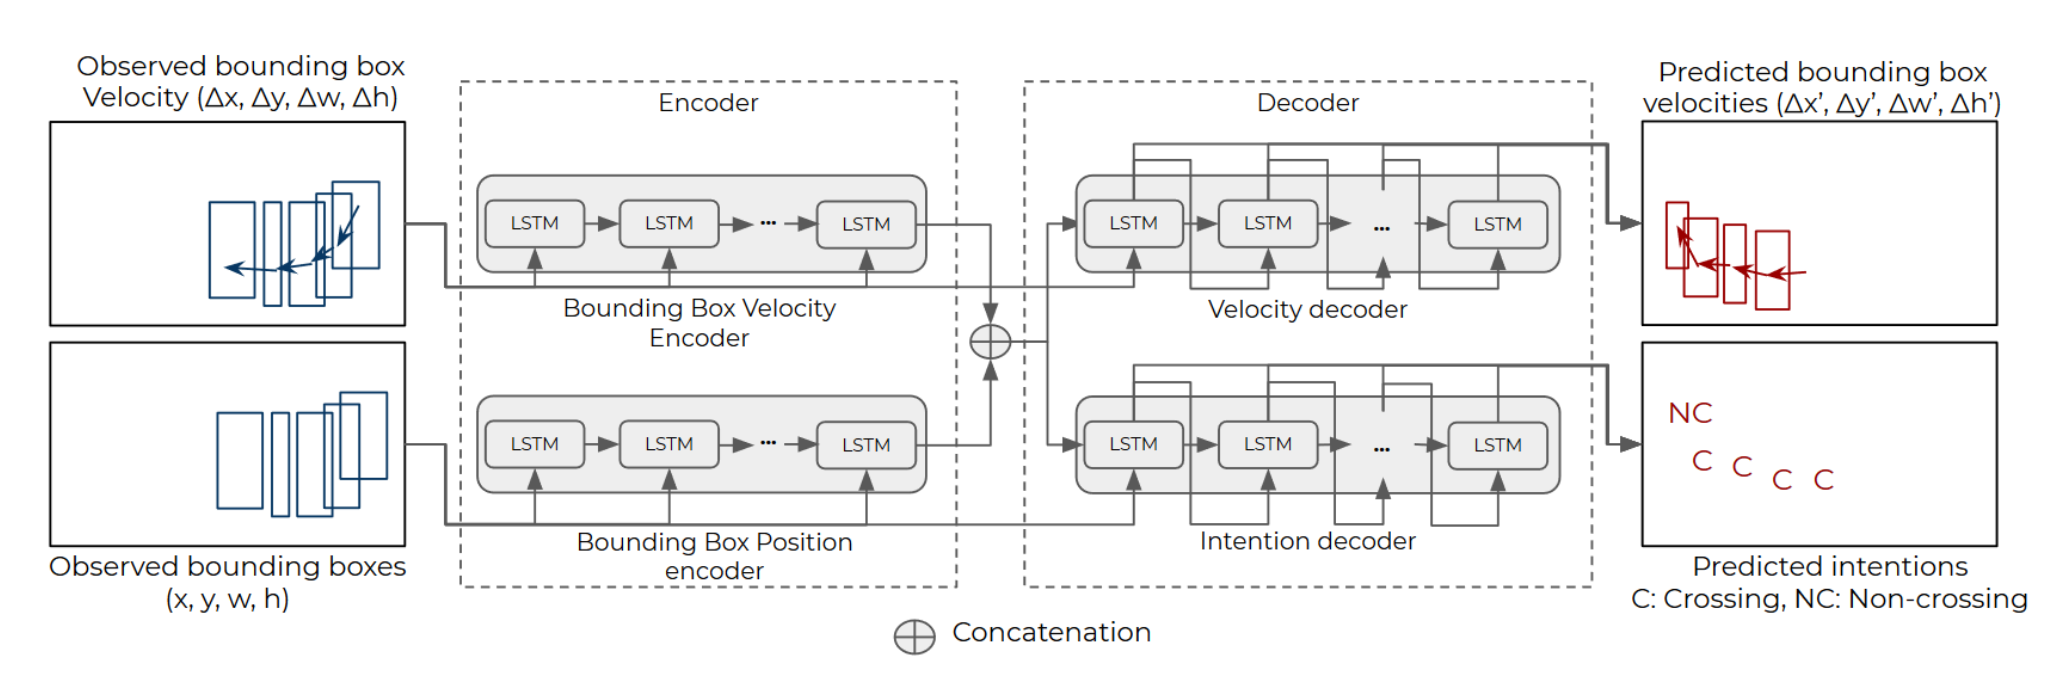
\includegraphics[width=1\textwidth]{figures/PV-LSTM.png}
    \caption{PV-LSTM Model Architecture. Source:~\citet{DBLP:journals/corr/abs-2010-10270}}\label{fig:pv-lstm}
\end{figure}

\noindent The PV-LSTM model was evaluated on the Citywalks dataset, and its performance
was compared against several baseline models. The results are summarised in
Table~\ref{tab:pv-lstm-results}, showcasing the model's effectiveness in
predicting pedestrian trajectories and intentions. The PV-LSTM model achieved
an Average Displacement Error (ADE) of 25.2 pixels and a Final Displacement
Error (FDE) of 49.9 pixels, with an Average Intersection Over Union (AIoU) of
40.2\%. Although the STED model slightly outperforms in AIoU and FIoU, the
PV-LSTM model provides a robust solution with competitive prediction accuracy,
while maintaining a simpler architecture.

\begin{table}[H]
    \centering
    \caption{Comparison of the performance of PV-LSTM with baseline models on the Citywalks dataset. }
    \begin{adjustbox}{max width=\textwidth}
        \begin{tabular}{lcccc}
            \toprule
            \textbf{Model}                                   & \textbf{ADE (pixels)} & \textbf{FDE (pixels)} & \textbf{AIoU (\%)} & \textbf{FIoU (\%)} \\ 
            \midrule
            CV-CS~\cite{DBLP:journals/corr/abs-2010-10270}   & 31.6                  & 57.6                  & 46.0               & 21.3               \\
            LKF~\cite{DBLP:journals/corr/abs-2010-10270}     & 32.9                  & 59.0                  & 43.9               & 20.1               \\
            STED~\cite{DBLP:journals/corr/abs-2010-10270}    & \textbf{26.0}         & \textbf{46.9}         & \textbf{51.8}      & \textbf{27.5}      \\
            PV-LSTM~\cite{DBLP:journals/corr/abs-2010-10270} & 25.2                  & 49.9                  & 40.2               & 20.3               \\
            \bottomrule
        \end{tabular}
    \end{adjustbox}
    \label{tab:pv-lstm-results}
\end{table}

\subsubsection*{Fusion-Gated Recurrent Unit (Fusion-GRU) Model}

\citet{FusionGRU} developed the Fusion-Gated Recurrent
Unit (Fusion-GRU) model to predict the future bounding boxes of traffic agents
in risky driving scenarios. As illustrated in Figure~\ref{fig:fusion-gru}, this model leverages multiple sources of
information, such as location-scale data, monocular depth information, and
optical flow data, to capture complex interactions among these cues and
transform them into meaningful hidden representations. This approach is
particularly suited for dealing with scenarios where the available observation
time is limited due to abrupt motion changes or tracking loss. 
The Fusion-GRU model consists of several components that work together to
predict future bounding boxes. The model takes input video sequences, extracts
depth maps, and calculates optical flow to capture motion dynamics. Bounding
boxes are detected and tracked using YOLOv5 and DeepSort, respectively. The
feature extractor processes both object-level and scene-level features using
ResNet50, transforming them into feature vectors. These vectors are then
concatenated and passed to the Fusion-GRU encoder, which integrates location,
scale, and distance information into hidden representations. 
The model also introduces an intermediary estimator, which generates
intermediate bounding boxes that help in capturing sequential dependencies
across frames. Additionally, a self-attention aggregation layer is employed to
reduce error accumulation by focusing on the most relevant information for
long-term predictions. Finally, a GRU decoder iteratively predicts the future
bounding boxes based on the aggregated feature vectors and the hidden
representations from the Fusion-GRU encoder.

\begin{figure}[H]
    \centering
    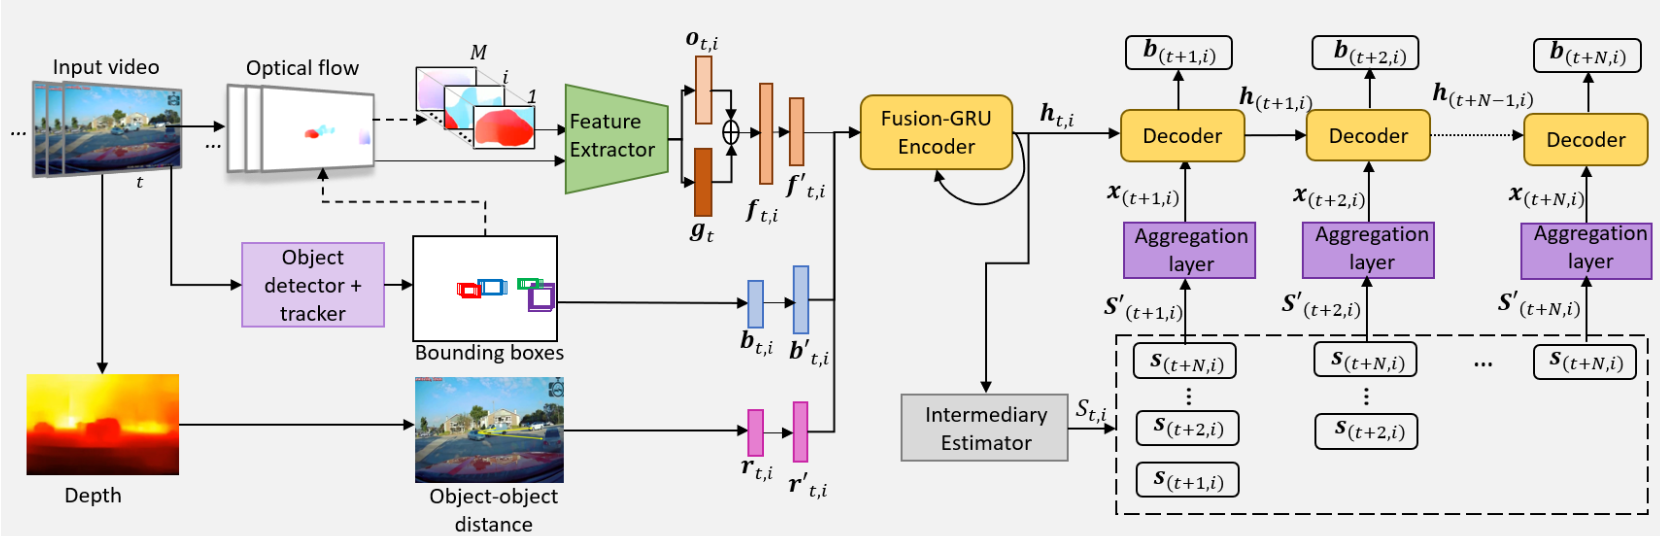
\includegraphics[width=1\textwidth]{figures/FusionGRU.png}
    \caption{Fusion-GRU model architecture. Source:~\citet{FusionGRU}}\label{fig:fusion-gru}
\end{figure}

\noindent The Fusion-GRU model is specifically designed to address the limitations of
traditional GRU-based models, which often suffer from performance degradation
over time. By integrating complex interactions among various input features and
employing self-attention mechanisms, the Fusion-GRU model enhances its ability
to predict future bounding boxes more accurately. This architecture is
particularly effective in cluttered and dynamic driving environments, where
understanding the relationships between different traffic agents and their
surroundings is crucial for accurate prediction. The Fusion-GRU model was
evaluated on two publicly available datasets, ROL (Risky Object Localization)~\cite{karim_am_net2023}
and HEV-I (Honda Egocentric View-Intersection)~\cite{yao2019egocentric, malla2019nemo}, demonstrating its superior
performance in predicting future bounding boxes compared to other
state-of-the-art models. The results are summarised in
Table~\ref{tab:fusion-gru-results}, which compares the performance of
Fusion-GRU with baseline models based on metrics such as Average Displacement
Error (ADE), Final Displacement Error (FDE), and Intersection over Union (IOU). The Fusion-GRU model achieved the lowest Average Displacement Error (ADE) and
Final Displacement Error (FDE) in both 0.5-second and 1-second prediction
horizons on the HEV-I dataset. It also exhibited the highest Final Intersection
over Union (FIoU) of 85.2\% in the 0.5-second horizon, indicating its strong
capability to accurately predict the future positions and scales of traffic
agents.

\begin{table}[H]
    \centering
    \caption{Comparison of the performance of Fusion-GRU with baseline models on the ROL and HEV-I datasets.}
    \begin{adjustbox}{max width=\textwidth}
        \begin{tabular}{lcccc}
            \toprule
            \textbf{Model}              & \textbf{ADE0.5 (pixels)} & \textbf{FDE0.5 (pixels)} & \textbf{FIoU0.5 (\%)} & \textbf{ADE1.0 (pixels)} \\ 
            \midrule
            FOL-X~\cite{FusionGRU}      & 6.7                      & 11.0                     & 85.0                  & 12.6                     \\
            SGDNet~\cite{FusionGRU}     & 6.3                      & --                       & --                    & 11.4                     \\
            Fusion-GRU~\cite{FusionGRU} & \textbf{5.5}             & \textbf{8.3}             & \textbf{85.2}         & \textbf{11.2}            \\
            \bottomrule
        \end{tabular}
    \end{adjustbox}
    \label{tab:fusion-gru-results}
\end{table}

%%%%%%%%%%%%%%%%%%%%%%%%%%%%%%%%%%%%%%%%%%%%%%%%%%%%%%%%%%%%%%%%%%%%%%%%%%%%%%%
%%%%%%%%%%%%%%%%%%%%%%%%%%%%%%%%% METHODOLOGY %%%%%%%%%%%%%%%%%%%%%%%%%%%%%%%%%
\chapter{Methodology}\label{chap:methodology}
\section{Dataset Configuration}
\subsection{Dataset Description}
The `Airbus A320 Refuelling Port' (AARP) dataset consists of 21 video sequences
captured inside or nearby an indoor hangar at the Aerospace Integration
Research Centre (AIRC). This dataset can be utilised for various purposes,
including but not limited to refuelling port detection and tracking, camera
pose estimation, and visual image processing. It is provided under the terms of
the UKRI funding agreement, as part of the ONEHeart project which aims to
develop an automated aircraft refuelling system based on computer vision and
robotics technology. Unauthorised use, distribution, or reproduction is
prohibited. The AARP dataset consists of 21 video sequences captured in an
indoor hangar at the Aerospace Integration Research Centre (AIRC). The videos
were recorded using an Intel® ${\text{RealSense}}^{\text{TM}}$
D435~\cite{IntelRealSense} (Shown in Figure~\ref{fig:intel-realsense-d435}),
which provides depth information in addition to RGB data. The target area for
detection and tracking is near the refuelling port of an Airbus A320 wing. The
videos were recorded under different lighting conditions, including indoor
artificial lighting and natural daylight, to simulate real-world scenarios. In
addition, the refuelling port was in different states (closed, open, and
semi-open) to capture a wide range of variations for training and testing
machine learning models.

\begin{figure}[H]
    \centering
    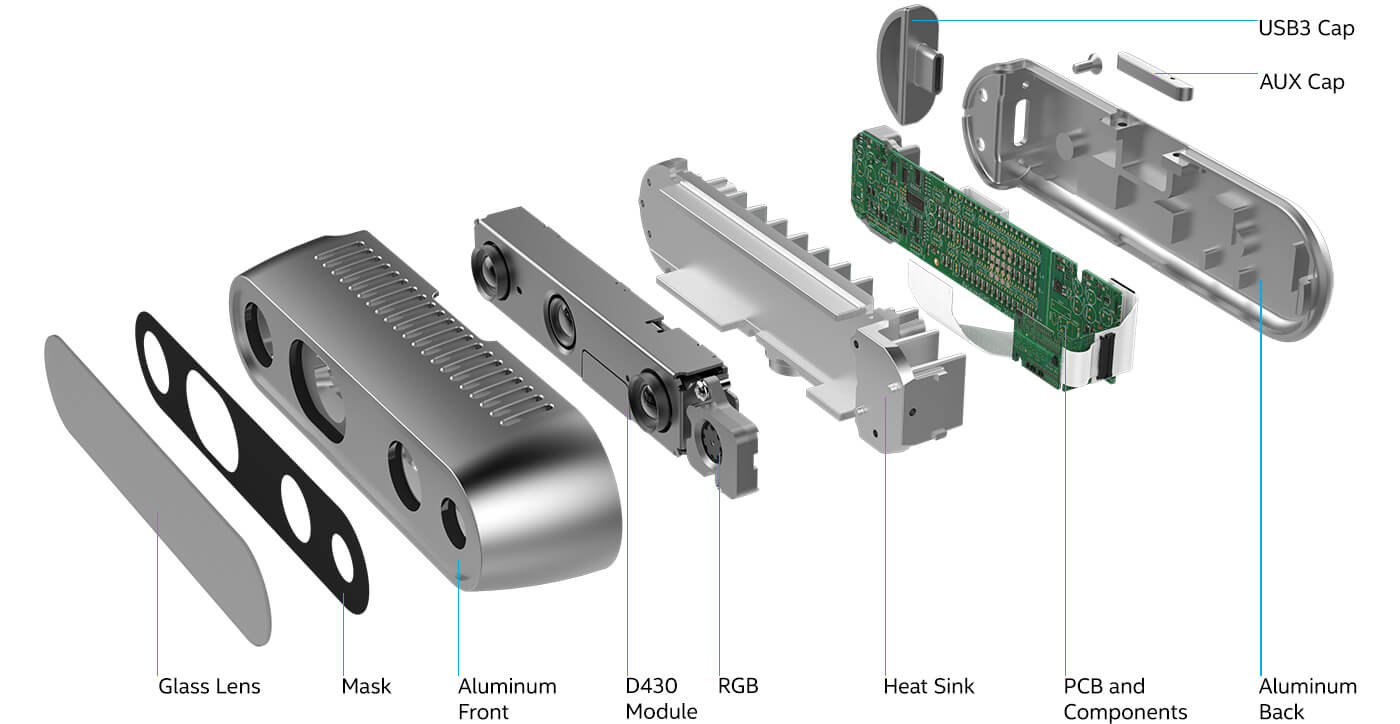
\includegraphics[width=0.8\textwidth]{figures/depth-camera-d435_details.jpg}
    \caption{Intel® ${\text{RealSense}}^{\text{TM}}$ D435 Depth Camera. Source: Intel}\label{fig:intel-realsense-d435}
\end{figure}

\newpage
\subsection{Data Annotation}
The AARP dataset provided for this project was not fully annotated. Therefore,
the first step in the data preparation process was to annotate the dataset.
This annotation process was crucial to enable the training of machine learning
models for accurate refuelling port detection and tracking. Initially, 100
frames from each video sequence were manually annotated. This involved labeling
the refuelling port in each frame, which required identifying and marking the
exact location of the refuelling port using bounding boxes. This was done using
the Label Studio tool, a powerful annotation platform that allows users to
create and manage annotations in images and videos. Label Studio was chosen for
its flexibility and ease of use. It supports various annotation formats and
integrates well with machine learning workflows. Users can draw bounding boxes
around objects of interest, in this case, the refuelling port, to create
labeled datasets. The initial manual annotations created a preliminary dataset.
This dataset was used to train a YOLOv10 (You Only Look Once, version 10) model
for refuelling port detection. The annotated dataset was used to train the
YOLOv10 model. The model learned to detect the refuelling port from the
annotated images, improving its accuracy with each training iteration. After
training the YOLOv10 model, it was implemented as a backend service for Label
Studio. This was deployed as a Docker container, allowing the model to be used
for automated annotation of the remaining images in the dataset. The model
predicted the location of the refuelling port in new frames, and these
predictions were used to annotate the rest of the dataset automatically. Each
automatically generated annotation was reviewed manually to ensure accuracy.
This review process involved verifying the location of the refuelling port in
each frame and making necessary corrections to the annotations. This thorough
quality control ensured that the entire dataset was consistently and accurately
labeled. This comprehensive annotation process ensured that the entire dataset
was accurately labeled, providing a robust foundation for training machine
learning models aimed at refuelling port detection and tracking. The
combination of manual and automated annotation techniques maximised efficiency
while maintaining high annotation quality. 

\newpage
\subsection{Summary of Available Videos}
Each video was assigned to a specific dataset (train, val, and test), with an
approximate split of 70\% for training, 15\% for validation, and 15\% for
testing. Table~\ref{tab:video_summary} presents the available videos in the
dataset along with the number of frames for each video and their assignment:

\begin{table}[H]
    \centering
    \begin{tabular}{@{}cccc@{}}
        \toprule
        \textbf{Type}      & \textbf{Video Name}                           & \textbf{Number of Frames} & \textbf{Assignment} \\ \midrule
        \textbf{Closed}    & \textbf{video\_lab\_platform\_1}              & \textbf{624}              & \textbf{train}      \\
        Closed             & video\_lab\_platform\_2                       & 639                       & train               \\
        Closed             & video\_lab\_platform\_5                       & 398                       & train               \\
        Closed             & video\_lab\_platform\_7                       & 412                       & train               \\
        Closed             & video\_lab\_platform\_8                       & 470                       & train               \\
        Closed             & video\_lab\_platform\_9                       & 373                       & train               \\
        Closed             & video\_lab\_manual\_1                         & 746                       & train               \\
        Closed             & video\_lab\_platform\_3                       & 569                       & val                 \\
        Closed             & video\_lab\_platform\_4                       & 247                       & val                 \\
        Closed             & video\_lab\_platform\_6                       & 303                       & test                \\
        Closed             & test\_outdoor1                                & 499                       & test                \\
        \textbf{Open}      & \textbf{video\_lab\_open\_1\_\_\_\_\_\_1}     & \textbf{497}              & \textbf{train}      \\
        Open               & video\_lab\_open\_1\_\_\_\_\_\_2              & 602                       & train               \\
        Open               & video\_lab\_open\_1\_\_\_\_\_\_3              & 313                       & train               \\
        Open               & video\_lab\_open\_1\_\_\_\_\_\_4              & 310                       & train               \\
        Open               & test\_indoor2                                 & 310                       & val                 \\
        Open               & test\_indoor1                                 & 314                       & test                \\
        \textbf{Semi-Open} & \textbf{video\_lab\_semiopen\_1\_\_\_\_\_\_1} & \textbf{739}              & \textbf{train}      \\
        Semi-Open          & video\_lab\_semiopen\_1\_\_\_\_\_\_2          & 439                       & train               \\
        Semi-Open          & video\_lab\_semiopen\_1\_\_\_\_\_\_4          & 372                       & val                 \\ 
        Semi-Open          & video\_lab\_semiopen\_1\_\_\_\_\_\_3          & 383                       & test                \\ \bottomrule
    \end{tabular}
    \caption{\centering Summary of available videos in the AARP dataset with their assignment.}
    \label{tab:video_summary}
\end{table}

\newpage
\subsection{Data Distribution}
Before balancing the data, the distribution of video frames across the
different datasets (train, validation, and test) for each state of the fueling
port (CLOSED, OPEN, and SEMI-OPEN) was as follows:
\begin{table}[H]
    \centering
    \begin{tabular}{@{}ccccc@{}}
        \toprule
        \textbf{Type}      & \textbf{Total Frames} & \textbf{Train} & \textbf{Test} & \textbf{Validation} \\ \midrule
        \textbf{CLOSED}    & 5280                  & 3662 (69.36\%) & 802 (15.19\%) & 816 (15.45\%)       \\ 
        \textbf{OPEN}      & 2346                  & 1722 (73.40\%) & 314 (13.38\%) & 310 (13.21\%)       \\ 
        \textbf{SEMI-OPEN} & 1933                  & 1178 (60.94\%) & 383 (19.81\%) & 372 (19.24\%)       \\ \bottomrule
    \end{tabular}
    \caption{\centering Distribution of frames across train, test, and validation sets for each state in the AARP dataset before balancing.}
    \label{tab:frame_distribution}
\end{table}

\noindent As shown in Table~\ref{tab:frame_distribution}, the dataset initially had an
imbalance in the number of frames for each state. For instance, the CLOSED
state had significantly more frames compared to the OPEN and SEMI-OPEN states.
This imbalance could lead to biased training and inaccurate model performance,
as the model might become overly familiar with the more prevalent CLOSED state
and underperform on the less represented states.

\subsection{Data Balancing}
To address this issue, a balancing strategy was employed to create a more
uniform dataset. The first step involved shuffling and subsetting each state
(CLOSED, OPEN, and SEMI-OPEN) to keep only the minimum number of frames for
each state. This ensured that the number of frames for each state was equal,
avoiding bias towards any particular state. The subsets were then merged to
create three balanced datasets: Training, Validation, and Test, each with an
equal number of frames for each state. Finally, the balanced datasets were
shuffled again and resized to maintain the required split ratio of 70\% for
training, 15\% for validation, and 15\% for testing. The balanced dataset will
be used for training and evaluating the object detection model, while the full
dataset will be utilised for sequence model training and framework evaluation.
The resulting distribution of frames across the train, test, and validation
sets for each state after balancing is shown in
Table~\ref{tab:balanced_frame_distribution}.
\begin{table}[H]
    \centering
    \begin{tabular}{@{}cc@{}}
        \toprule
        \textbf{Dataset} & \textbf{Total Frames} \\ \midrule
        \textbf{Train}   & 3534 (69.57\%)        \\ 
        \textbf{Test}    & 773  (15.22\%)        \\ 
        \textbf{Val}     & 773  (15.22\%)        \\ \bottomrule
    \end{tabular}
    \caption{\centering Distribution of frames across train, test, and validation sets for each state in the AARP dataset after balancing.}
    \label{tab:balanced_frame_distribution}
\end{table}

\noindent The primary reason for balancing the dataset is to ensure that the object
detection model is equally trained on all states of the refuelling port. An
imbalanced dataset could cause the model to perform well on the more common
states (like CLOSED) while underperforming on the less common states (like OPEN
and SEMI-OPEN). By balancing the dataset, the model has an equal opportunity to
learn from all states, improving its generalisation and robustness. 

\subsection{Example Images from the Datase}
\noindent Figure~\ref{fig:grid-closed-images}, Figure~\ref{fig:grid-semi-open-images}, and
Figure~\ref{fig:grid-open-images} show annotated images of the refuelling port
in the CLOSED, SEMI-OPEN, and OPEN states, respectively.
\begin{figure}[H]
    \centering
    \includegraphics[width=0.47\textwidth]{figures/grid\_closed\_images.png}
    \caption{Annotated images of the refuelling port in the CLOSED state.}~\label{fig:grid-closed-images}
\end{figure}

\begin{figure}[H]
    \centering
    \includegraphics[width=0.47\textwidth]{figures/grid\_semiopen\_images.png}
    \caption{Annotated images of the refuelling port in the SEMI-OPEN state.}~\label{fig:grid-semi-open-images}
\end{figure}

\begin{figure}[H]
    \centering
    \includegraphics[width=0.47\textwidth]{figures/grid\_open\_images.png}
    \caption{Annotated images of the refuelling port in the OPEN state.}~\label{fig:grid-open-images}
\end{figure}

\subsection{Temporal Dynamics Analysis of the Refuelling Port}
\begin{figure}[H]
    \centering
    \begin{subfigure}[t]{0.65\textwidth}
        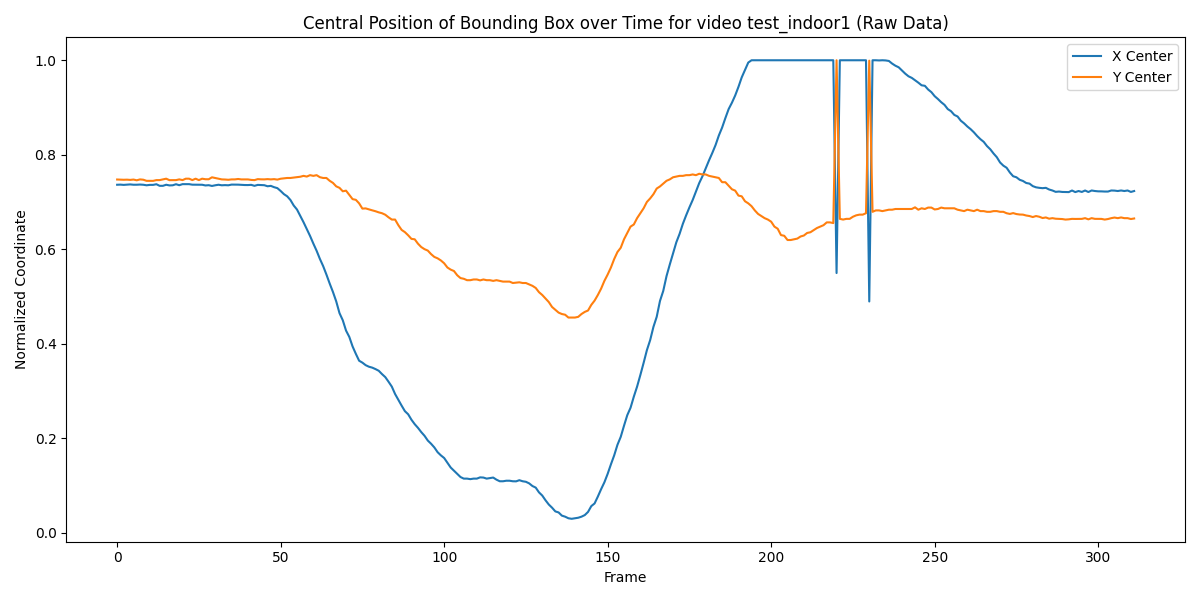
\includegraphics[width=\textwidth]{figures/bbox_metrics/test_indoor1 (Raw Data)_central_position.png}
        \caption{Central Position over Time without Filter.}
        \label{fig:central-position-test-indoor1-raw}
    \end{subfigure}
    \hfill
    \begin{subfigure}[t]{0.65\textwidth}
        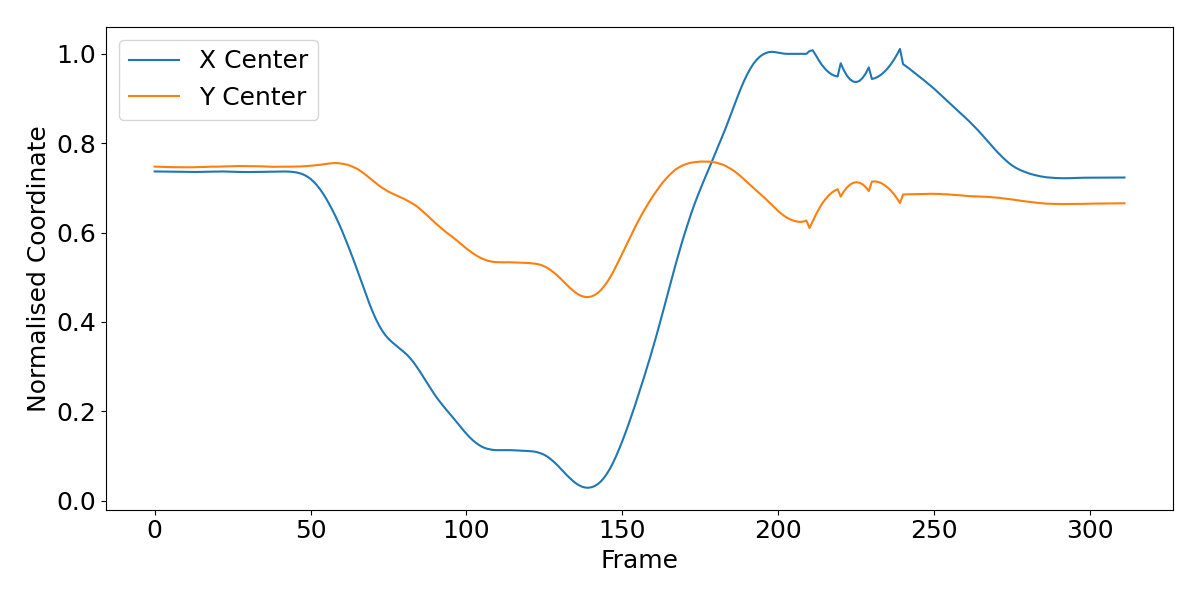
\includegraphics[width=\textwidth]{figures/bbox_metrics/test_indoor1 (Savgol Filter)_central_position.png}
        \caption{Central Position over Time with Savitzky-Golay Filter.}
        \label{fig:central-position-test-indoor1-savgol}
    \end{subfigure}
    \vfill
    \begin{subfigure}[t]{0.65\textwidth}
        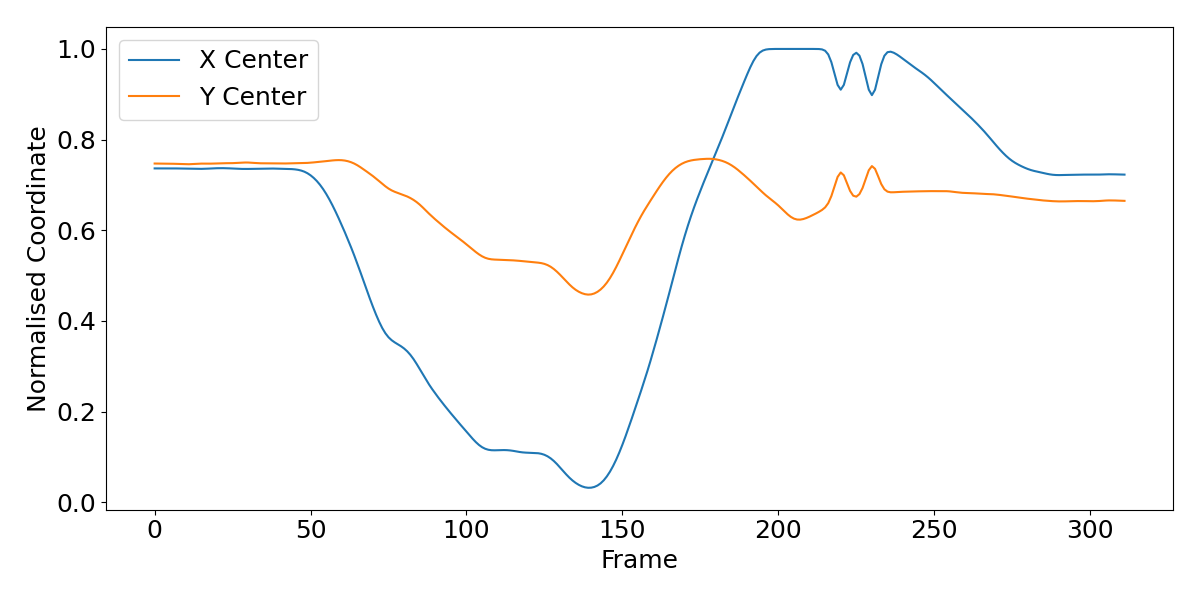
\includegraphics[width=\textwidth]{figures/bbox_metrics/test_indoor1 (Gaussian Filter)_central_position.png}
        \caption{Central Position over Time with Gaussian Filter.}
        \label{fig:central-position-test-indoor1-gaussian}
    \end{subfigure}
    \hfill
    \begin{subfigure}[t]{0.65\textwidth}
        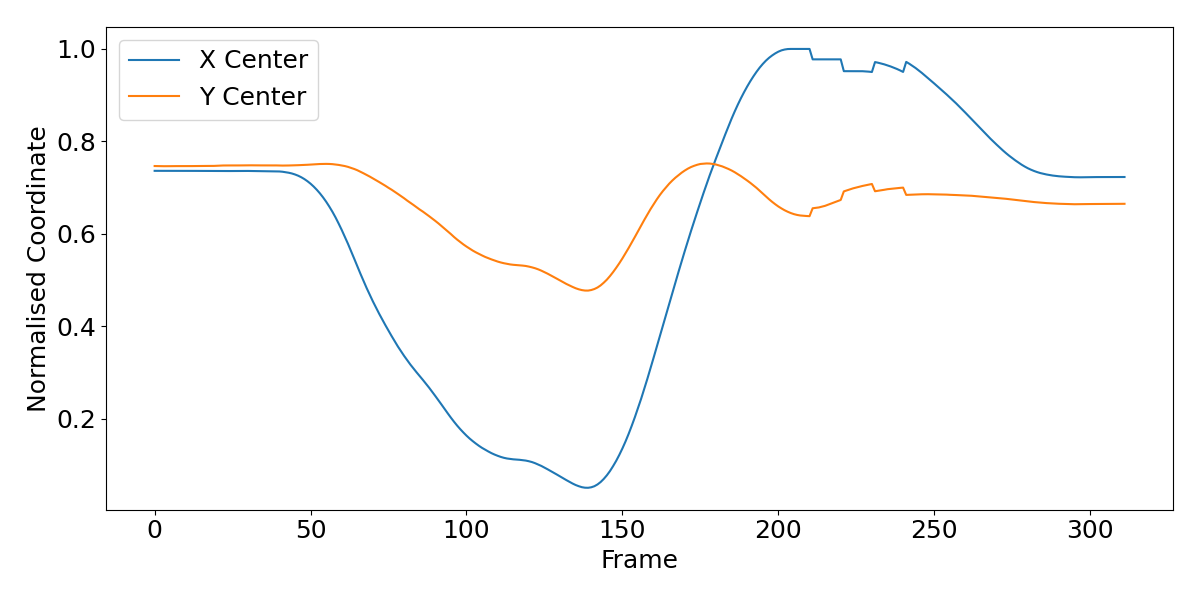
\includegraphics[width=\textwidth]{figures/bbox_metrics/test_indoor1 (Rolling Mean Filter)_central_position.png}
        \caption{Central Position over Time with Rolling Mean Filter.}
        \label{fig:central-position-test-indoor1-rolling}
    \end{subfigure}
    \caption{Temporal analysis of refuelling port central position in video \textit{test\_indoor1}.}
    \label{fig:central-position-test-indoor1}
\end{figure}

\begin{figure}[H]
    \centering
    \begin{subfigure}[t]{0.65\textwidth}
        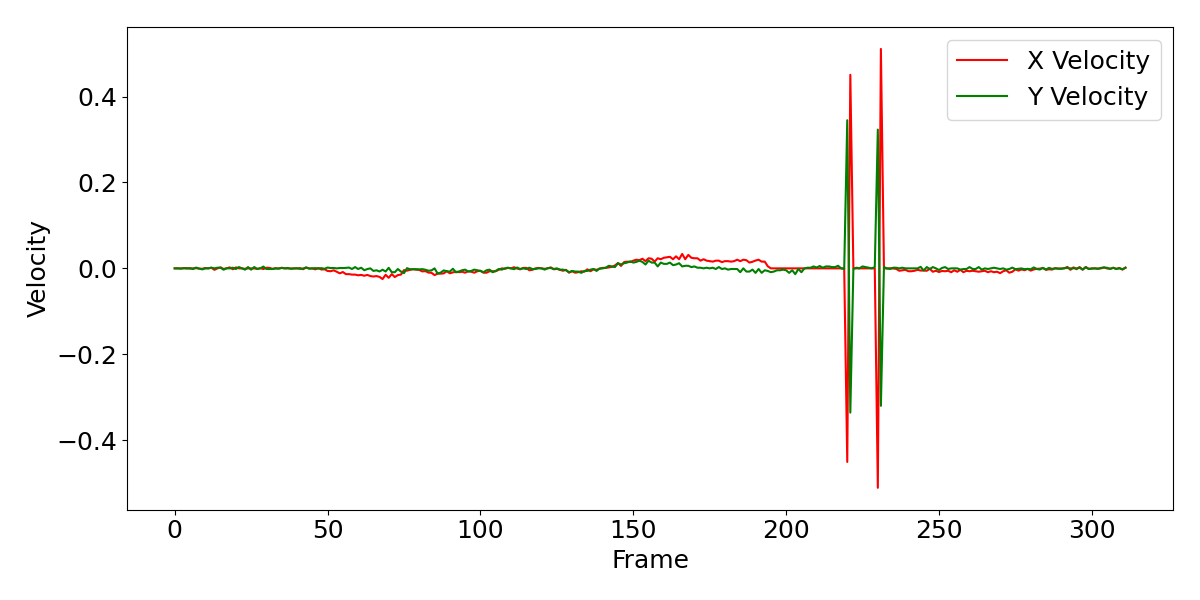
\includegraphics[width=\textwidth]{figures/bbox_metrics/test_indoor1 (Raw Data)_velocity.png}
        \caption{Velocity over Time without Filter.}
        \label{fig:velocity-test-indoor1-raw}
    \end{subfigure}
    \hfill
    \begin{subfigure}[t]{0.65\textwidth}
        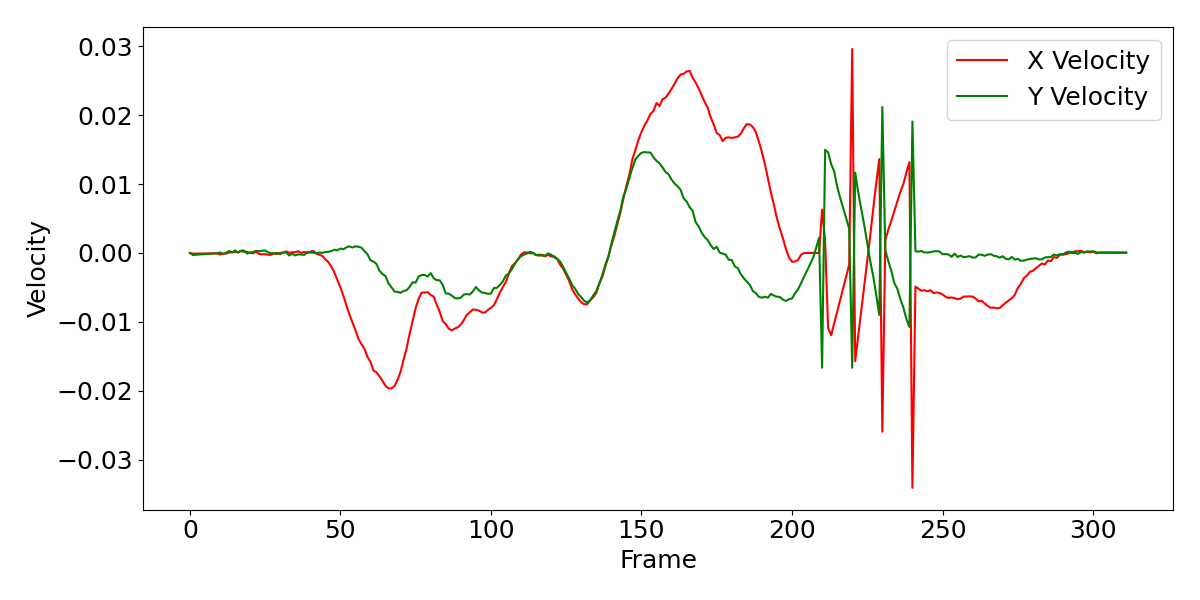
\includegraphics[width=\textwidth]{figures/bbox_metrics/test_indoor1 (Savgol Filter)_velocity.png}
        \caption{Velocity over Time with Savitzky-Golay Filter.}
        \label{fig:velocity-test-indoor1-savgol}
    \end{subfigure}
    \vfill
    \begin{subfigure}[t]{0.65\textwidth}
        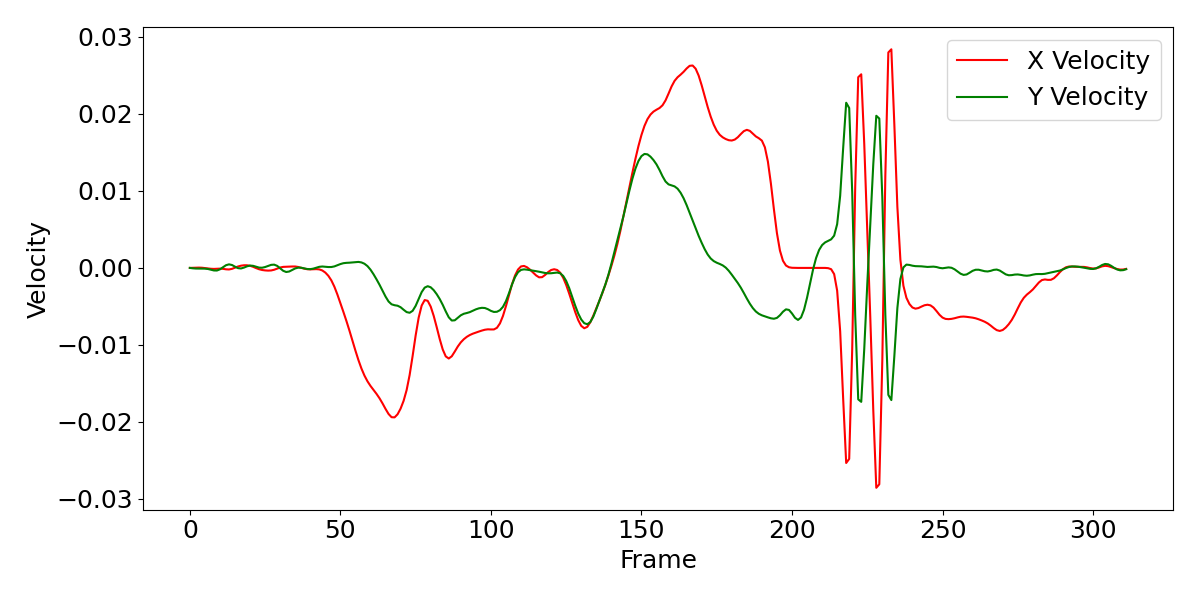
\includegraphics[width=\textwidth]{figures/bbox_metrics/test_indoor1 (Gaussian Filter)_velocity.png}
        \caption{Velocity over Time with Gaussian Filter.}
        \label{fig:velocity-test-indoor1-gaussian}
    \end{subfigure}
    \hfill
    \begin{subfigure}[t]{0.65\textwidth}
        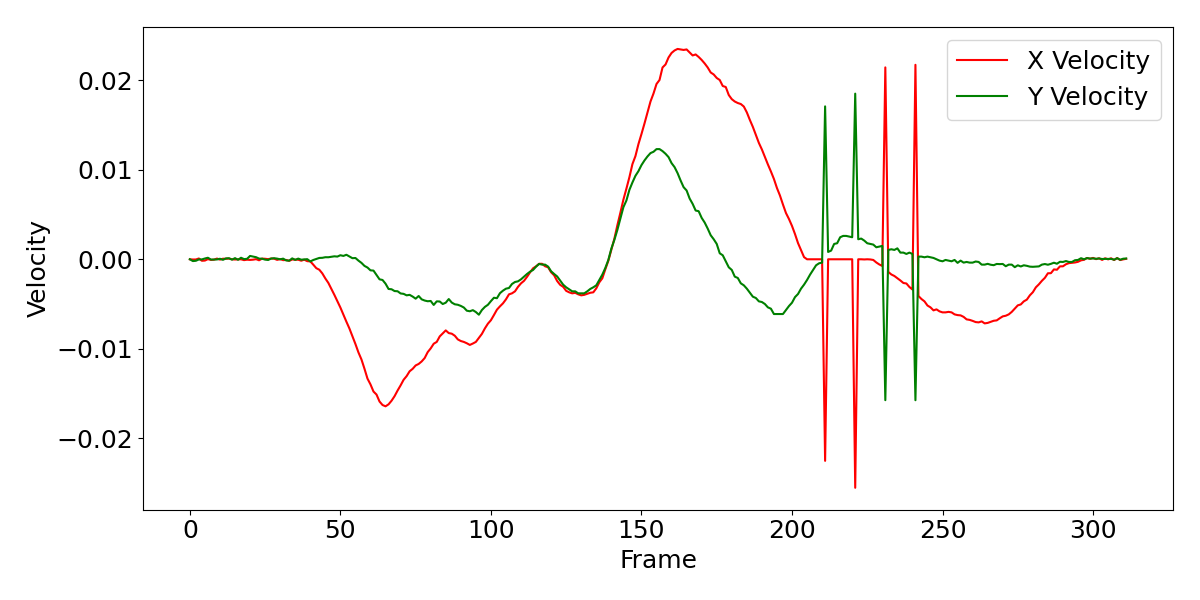
\includegraphics[width=\textwidth]{figures/bbox_metrics/test_indoor1 (Rolling Mean Filter)_velocity.png}
        \caption{Velocity over Time with Rolling Mean Filter.}
        \label{fig:velocity-test-indoor1-rolling}
    \end{subfigure}
    \caption{Temporal analysis of refuelling port velocity in video \textit{test\_indoor1}.}
    \label{fig:velocity-test-indoor1}
\end{figure}

\begin{figure}[H]
    \centering
    \begin{subfigure}[t]{0.65\textwidth}
        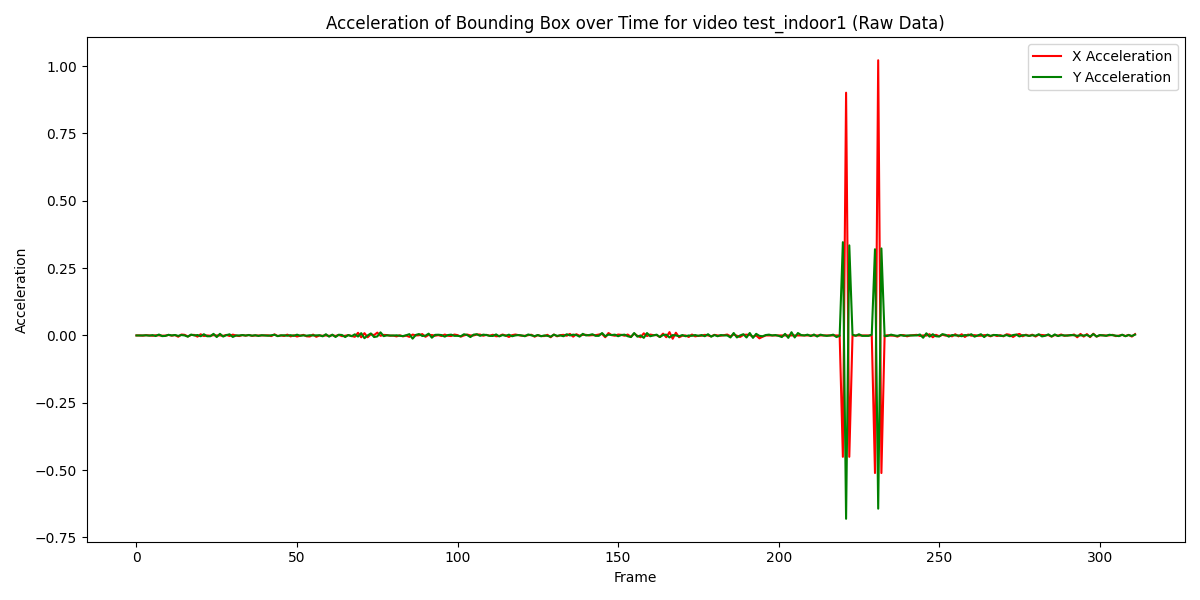
\includegraphics[width=\textwidth]{figures/bbox_metrics/test_indoor1 (Raw Data)_acceleration.png}
        \caption{Acceleration over Time without Filter.}
        \label{fig:acceleration-test-indoor1-raw}
    \end{subfigure}
    \hfill
    \begin{subfigure}[t]{0.65\textwidth}
        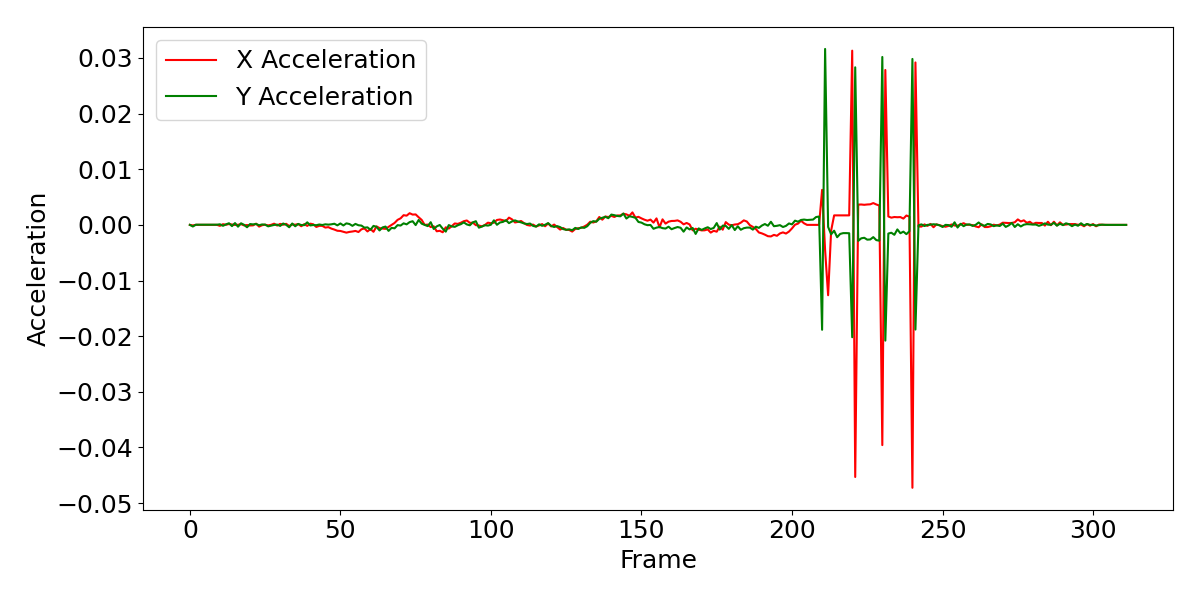
\includegraphics[width=\textwidth]{figures/bbox_metrics/test_indoor1 (Savgol Filter)_acceleration.png}
        \caption{Acceleration over Time with Savitzky-Golay Filter.}
        \label{fig:acceleration-test-indoor1-savgol}
    \end{subfigure}
    \vfill
    \begin{subfigure}[t]{0.65\textwidth}
        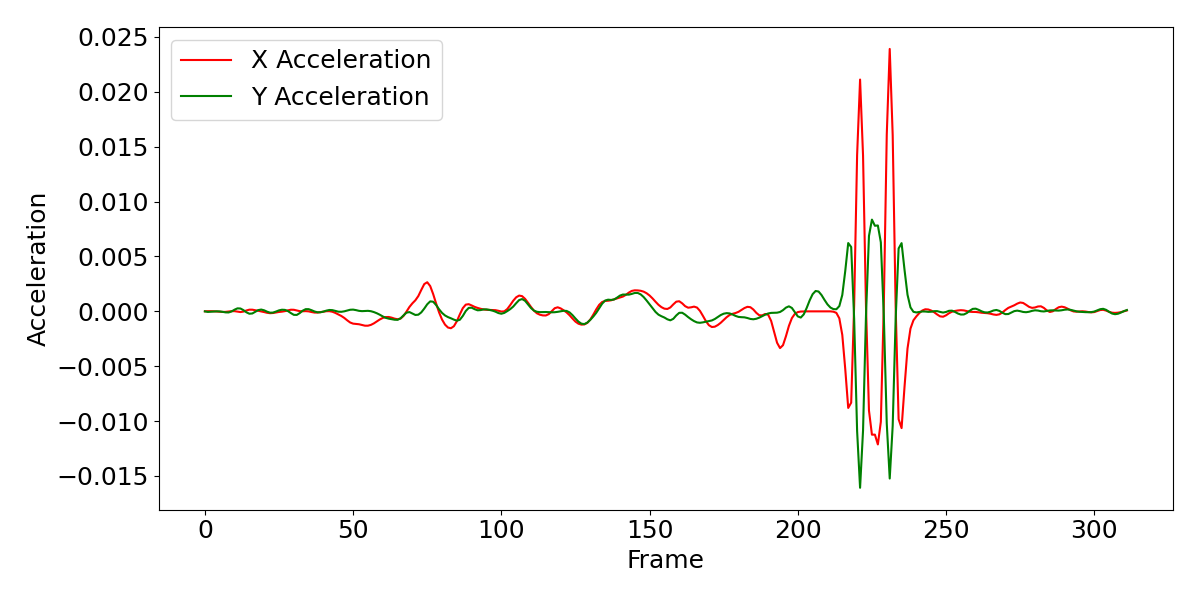
\includegraphics[width=\textwidth]{figures/bbox_metrics/test_indoor1 (Gaussian Filter)_acceleration.png}
        \caption{Acceleration over Time with Gaussian Filter.}
        \label{fig:acceleration-test-indoor1-gaussian}
    \end{subfigure}
    \hfill
    \begin{subfigure}[t]{0.65\textwidth}
        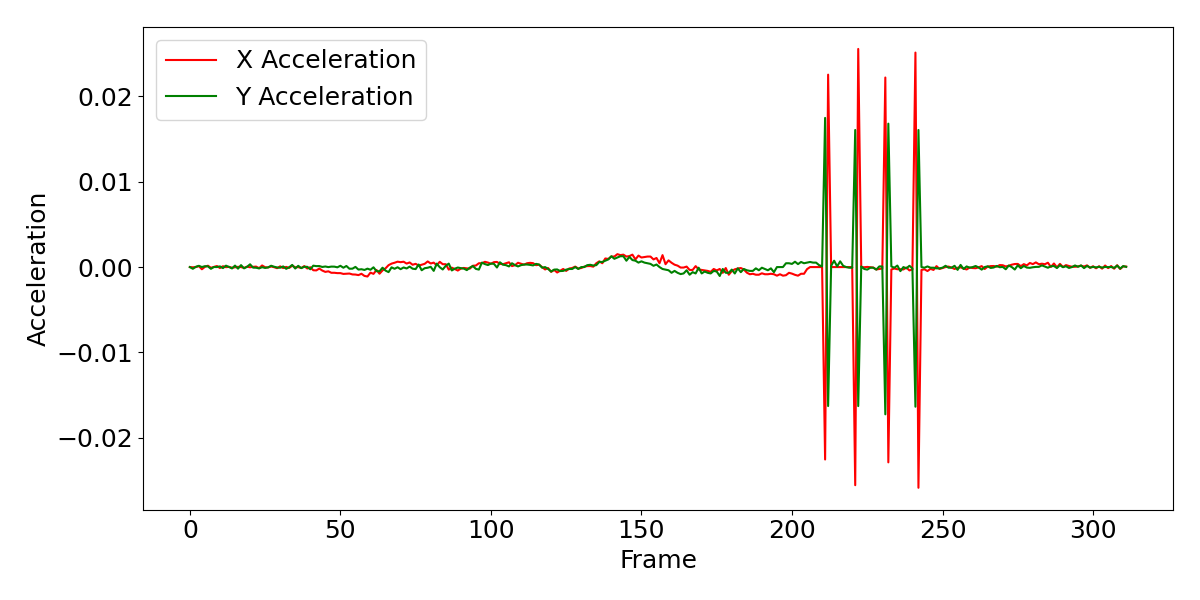
\includegraphics[width=\textwidth]{figures/bbox_metrics/test_indoor1 (Rolling Mean Filter)_acceleration.png}
        \caption{Acceleration over Time with Rolling Mean Filter.}
        \label{fig:acceleration-test-indoor1-rolling}
    \end{subfigure}
    \caption{Temporal analysis of refuelling port acceleration in video \textit{test\_indoor1}.}
    \label{fig:acceleration-test-indoor1}
\end{figure}

\begin{figure}[H]
    \centering
    \begin{subfigure}[t]{0.65\textwidth}
        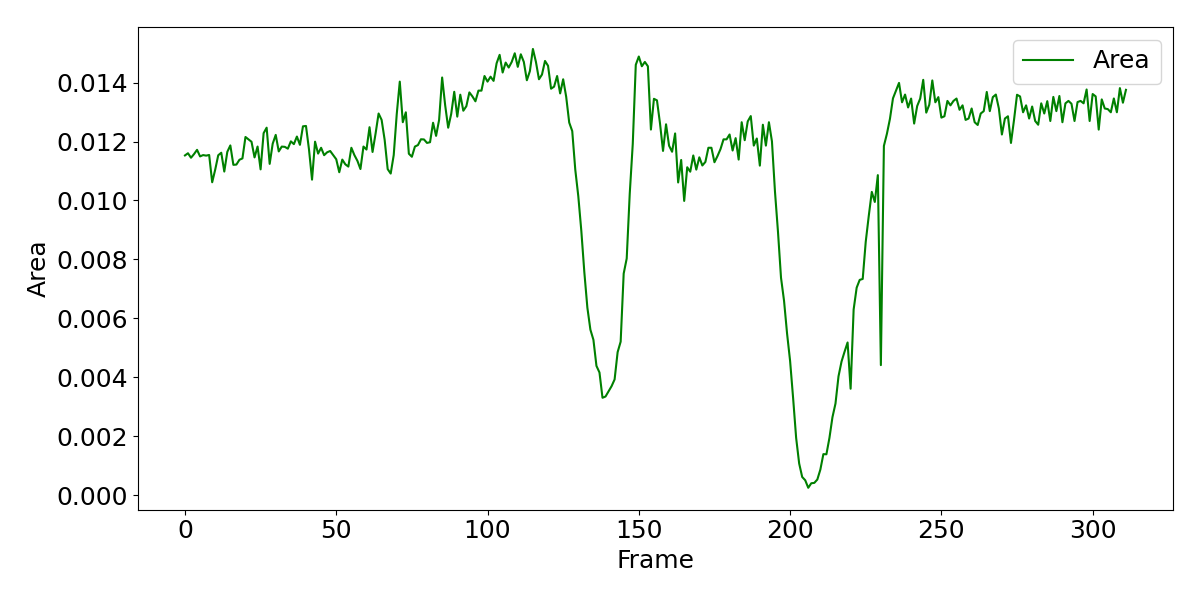
\includegraphics[width=\textwidth]{figures/bbox_metrics/test_indoor1 (Raw Data)_area.png}
        \caption{Area over Time without Filter.}
        \label{fig:size-test-indoor1-raw}
    \end{subfigure}
    \hfill
    \begin{subfigure}[t]{0.65\textwidth}
        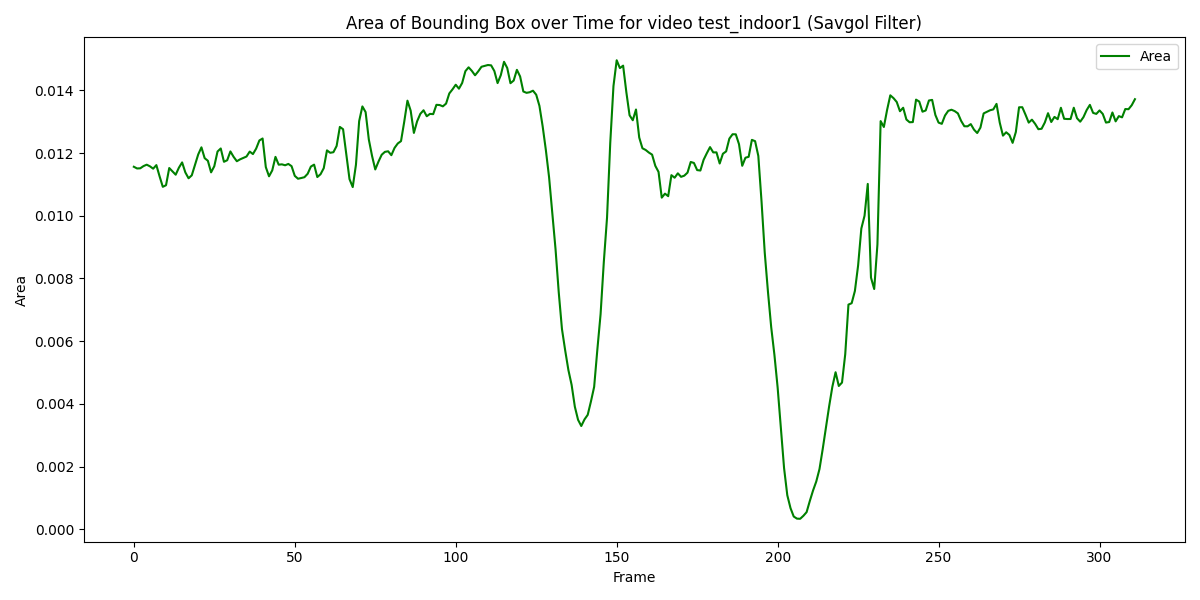
\includegraphics[width=\textwidth]{figures/bbox_metrics/test_indoor1 (Savgol Filter)_area.png}
        \caption{Area over Time with Savitzky-Golay Filter.}
        \label{fig:size-test-indoor1-savgol}
    \end{subfigure}
    \vfill
    \begin{subfigure}[t]{0.65\textwidth}
        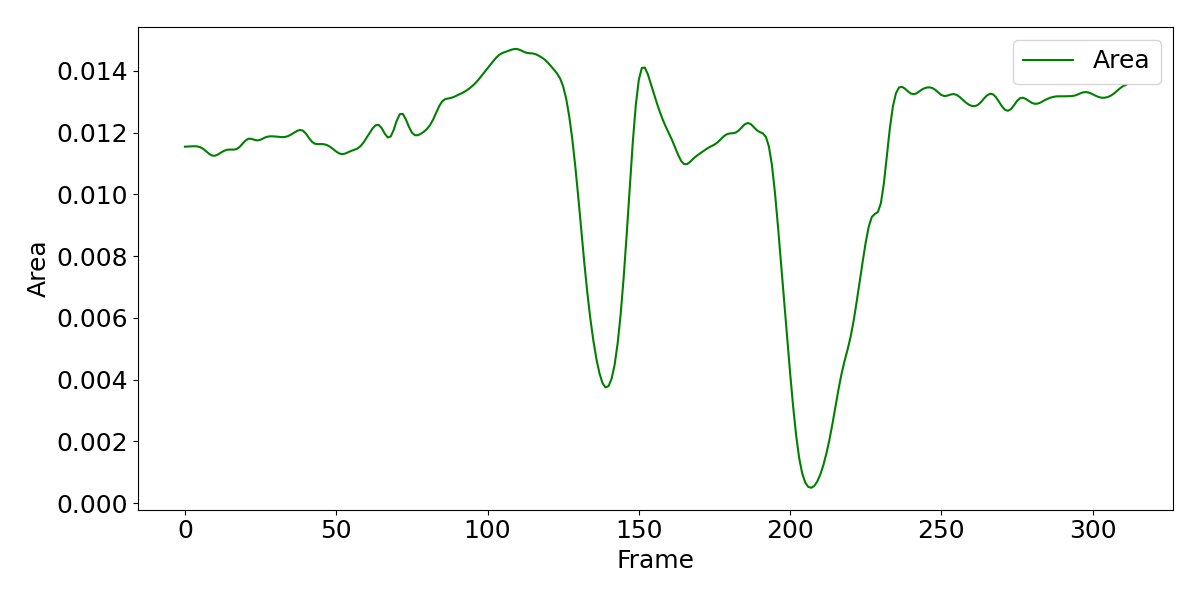
\includegraphics[width=\textwidth]{figures/bbox_metrics/test_indoor1 (Gaussian Filter)_area.png}
        \caption{Area over Time with Gaussian Filter.}
        \label{fig:size-test-indoor1-gaussian}
    \end{subfigure}
    \hfill
    \begin{subfigure}[t]{0.65\textwidth}
        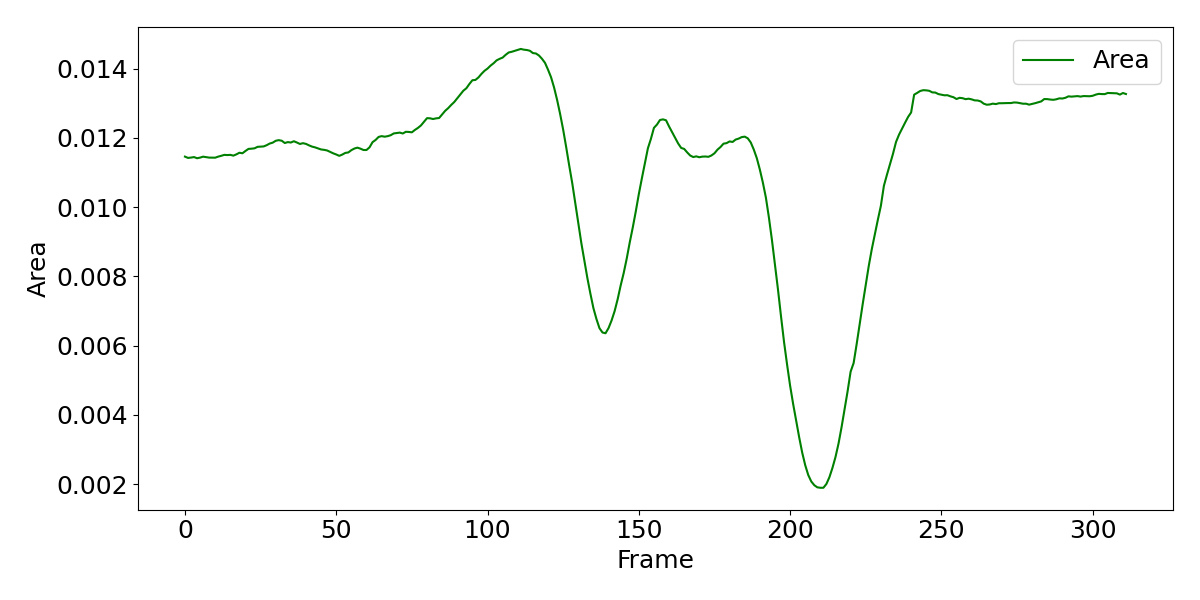
\includegraphics[width=\textwidth]{figures/bbox_metrics/test_indoor1 (Rolling Mean Filter)_area.png}
        \caption{Area over Time with Rolling Mean Filter.}
        \label{fig:size-test-indoor1-rolling}
    \end{subfigure}
    \caption{Temporal analysis of refuelling port size in video \textit{test\_indoor1}.}
    \label{fig:size-test-indoor1}
\end{figure}

In this analysis, different filters were applied to the refuelling port data to
improve the clarity and reliability of the temporal dynamics, which are
essential for training sequence models. The filters tested include the
Savitzky-Golay filter, Gaussian filter, and Rolling Mean filter. Each of these
filters has unique characteristics in how they reduce noise and preserve data
trends, making them suitable for different analytical needs. The Savitzky-Golay
filter smooths the data by applying a polynomial regression to a sliding
window, effectively reducing high-frequency noise while preserving the shape
and essential characteristics of the signal~\cite{Savitzky1964, 5888646}. This
makes it ideal for situations where maintaining the integrity of the data trend
is critical. The Gaussian filter, on the other hand, applies a Gaussian
function to smooth the data, which helps in reducing noise by softening sharp
edges and making the overall trend more observable, though at the cost of
potentially blurring finer details~\cite{8378142}. The Rolling Mean filter
computes a moving average over the data, which smooths out short-term
fluctuations and emphasises longer-term trends, but this method can sometimes
oversmooth the data, potentially obscuring subtle but important
variations~\cite{smith1999dsp}. 

Firstly, the central position of the refuelling port was tracked over time to
assess its movement along the X and Y axes, as shown in
Figure~\ref{fig:central-position-test-indoor1}. The raw data
(Figure~\ref{fig:central-position-test-indoor1-raw}) displayed substantial
noise, particularly in the X coordinate, which made it challenging to discern
the true movement of the refuelling port. Applying the Savitzky-Golay filter
(Figure~\ref{fig:central-position-test-indoor1-savgol}) effectively smoothed
out the noise while retaining the essential trend of the central position,
allowing for the preservation of important variations in the data that might
indicate significant movement patterns. In contrast, the Rolling Mean filter
(Figure~\ref{fig:central-position-test-indoor1-rolling}) offered a similar
level of smoothing but tended to oversmooth the data, potentially obscuring
critical inflection points that are necessary for accurate predictions. The
Gaussian filter (Figure~\ref{fig:central-position-test-indoor1-gaussian}) also
provided smoothing, but with a slight reduction in the preservation of smaller
fluctuations, which could be significant for predictive tasks. Then, velocity
was analysed by differentiating the central position over time, as depicted in
Figure~\ref{fig:velocity-test-indoor1}. The raw velocity data
(Figure~\ref{fig:velocity-test-indoor1-raw}) was noisy, with sharp spikes
indicating erratic changes in speed that could be artifacts. The Savitzky-Golay
filter (Figure~\ref{fig:velocity-test-indoor1-savgol}) smoothed these spikes,
making the data more interpretable and highlighting consistent trends that
would help the sequence model learn meaningful patterns. The Gaussian filter
(Figure~\ref{fig:velocity-test-indoor1-gaussian}) provided a similar smoothing
effect, ensuring gradual and reflective changes in velocity. However, it
slightly dampened the sharp transitions that might be relevant for identifying
sudden movements. The Rolling Mean filter
(Figure~\ref{fig:velocity-test-indoor1-rolling}) effectively reduced noise but
risked removing crucial data about sudden movements necessary for accurate
predictions. Acceleration, derived as the second derivative of the central
position, was analysed in its raw form
(Figure~\ref{fig:acceleration-test-indoor1-raw}) and through the application of
filters (Figures~\ref{fig:acceleration-test-indoor1-savgol},
\ref{fig:acceleration-test-indoor1-gaussian}, and
\ref{fig:acceleration-test-indoor1-rolling}). The raw acceleration data
exhibited extreme spikes, which were effectively smoothed by the Savitzky-Golay
filter, resulting in a clearer signal that still captured essential trends. The
Gaussian filter also provided a comparable smoothing effect, but the Rolling
Mean filter’s tendency to oversmooth could obscure real changes in acceleration
that are critical for the model to learn. Finally, the area of the refuelling port, representing its size over time, was
analysed in Figure~\ref{fig:size-test-indoor1}. The raw area data fluctuated
considerably, with abrupt changes likely due to noise or occlusions in the
video data (Figure~\ref{fig:size-test-indoor1-raw}). Smoothing was necessary to
understand the true size changes, with the Savitzky-Golay filter proving
effective in reducing noise while preserving key trends, making the data more
reliable for training the sequence model. The Gaussian filter also performed
well, particularly in moderately noisy data, but the Rolling Mean filter’s
tendency to oversmooth suggests it may not be suitable when detailed temporal
patterns are important.

In conclusion, the Savitzky-Golay filter consistently balanced noise reduction
with the preservation of critical temporal dynamics, making it the recommended
preprocessing method for training a sequence model. The Gaussian filter also
performed adequately, especially in scenarios where reducing noise is a
priority, but it should be used with caution to avoid over-smoothing important
data features. The Rolling Mean filter, while useful in certain contexts, often
risked obscuring meaningful patterns, making it less suitable for applications
requiring detailed temporal analysis. Therefore, the Savitzky-Golay filter will
be used here for preparing the data to train the sequence model to predict the
refuelling port’s future positions and sizes.

\section{Framework Design}

\begin{figure}[H]
    \centering
    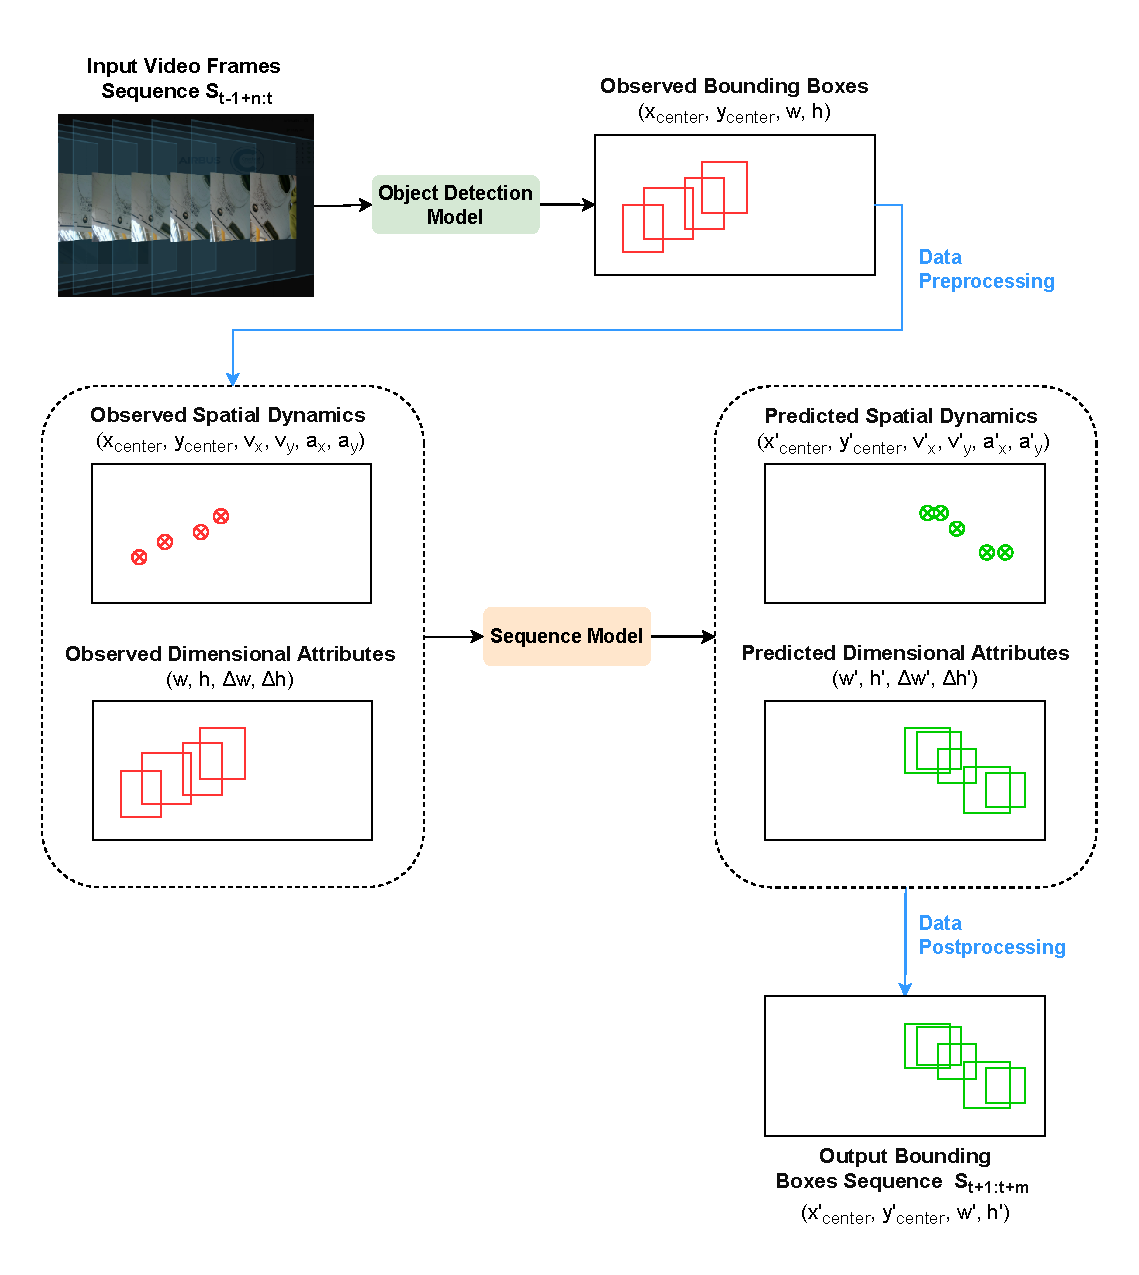
\includegraphics[width=1\textwidth]{figures/FrameworkWorkflow.drawio.pdf}
    \caption{Framework Workflow}\label{fig:framework-workflow}
\end{figure}

The proposed framework, illustrated in Figure~\ref{fig:framework-workflow}, is
designed to predict the future positions of the refuelling port’s bounding
boxes across the next \(m\) frames of a video stream. The objective is to
forecast a sequence of future bounding boxes, \(\mathbf{S}_{t+1:t+m} =
\{\mathbf{b}_{t+1}, \dots, \mathbf{b}_{t+m}\}\), based on the observed bounding
boxes from the past \(n\) frames, \(\mathbf{S}_{t-n+1:t} =
\{\mathbf{b}_{t-n+1}, \dots, \mathbf{b}_{t}\}\). The process begins with an
input video sequence, which is analysed on a frame-by-frame basis. An object
detection model first identifies and locates the bounding boxes of the
refuelling port in each frame. At any given time step \(t\), the observed
bounding box is denoted as \(\mathbf{b}_t = [x_t, y_t, w_t, h_t]\), where
\((x_t, y_t)\) represent the centre coordinates of the bounding box, and
\(w_t\) and \(h_t\) represent the width and height of the bounding box,
respectively. These detected bounding boxes are then formatted into input
vectors suitable for the sequence model. The sequence model is responsible for
predicting the future spatial positions and dimensions of the refuelling port’s
bounding boxes. Finally, these predictions are refined through post-processing
steps to produce the final bounding box forecasts for the subsequent frames.

\section{Object Detection Model Fine-tuning}
A fine-tuned YOLOv10S model is used to detect the refuelling port within the
video frames, as depicted in the object detection model section of
Figure~\ref{fig:framework-workflow}. As highlighted in the literature review,
YOLOv10 represents the latest advancement in object detection technology,
offering an optimal balance between speed and accuracy. The YOLOv10S variant is
particularly well-suited for real-time applications, especially on
resource-constrained embedded devices, due to its lightweight architecture. The
model is fine-tuned through transfer learning on the AARP dataset, enabling
precise detection of the refuelling port within the video frames. This
fine-tuning process ensures that the model meets the demands of real-time video
analysis with both accuracy and responsiveness. The implementation uses the
Ultralytics YOLOv10 framework~\cite{Jocher_Ultralytics_YOLO_2023}, which
provides a reliable and efficient pipeline for both training and inference.
This framework optimises detection performance and guarantees robust operation
in different scenarios.

\section{Sequence Model Design}

This thesis introduces a novel deep learning sequence model, named
\textit{SizPos-GRU}, specifically designed for predicting the future positions
and sizes of a unique object in a video stream. The \textit{SizPos-GRU} model
leverages an encoder-attention-decoder architecture to effectively capture both
temporal dependencies and spatial relationships in the data. The
\textit{SizPos-GRU} framework consists of four main components: two encoders,
an attention mechanism, and two decoders. Each component is meticulously
designed to handle specific aspects of the sequence modelling task, from
encoding input sequences to generating context-aware predictions. This custom
architecture ensures accurate and efficient prediction of future object
trajectories and dimensions within video streams.

\begin{figure}[H]
    \centering
    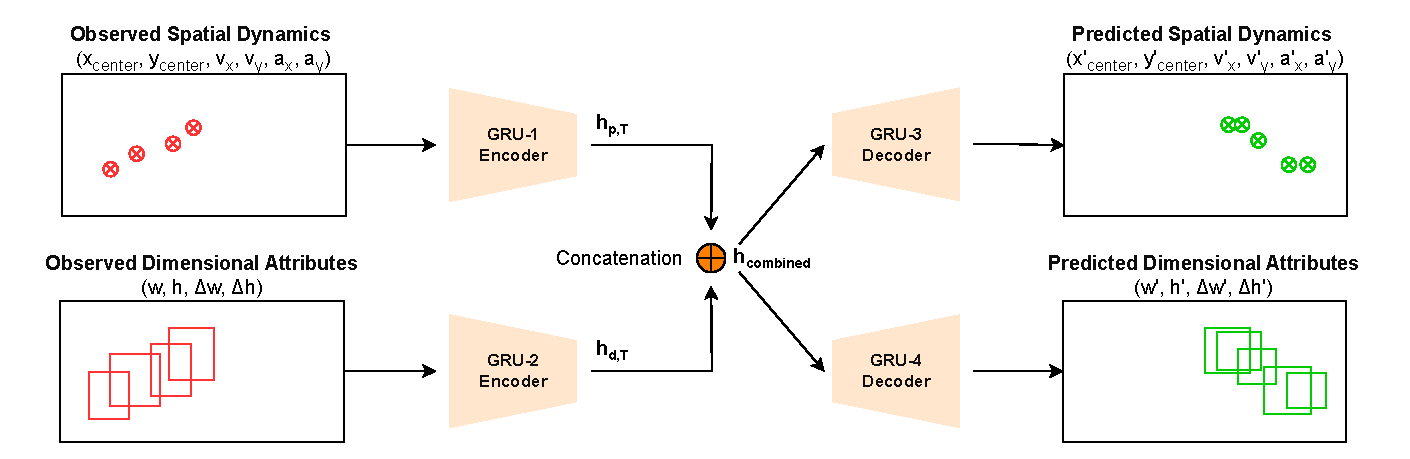
\includegraphics[width=1\textwidth]{figures/GRUSizPos.drawio.pdf}
    \caption{\textit{SizPos-GRU} model Architecture}\label{fig:sizpos-gru}
\end{figure}

\subsection{Input Representation}
\noindent The \textit{SizPos-GRU} model expects two types of input sequences to predict future positions and sizes of an object. The first input captures the spatial dynamics of the object, including its position, velocity, and acceleration. The second input focuses on the object's dimensional attributes, such as its width and height, and changes in these dimensions over time.

\subsubsection*{Spatial Dynamics Vector}
\noindent The spatial dynamics vector at time $t$, denoted as $\mathbf{p}_t$, represents the position, velocity, and acceleration of the bounding box center. It is defined as follows:

\begin{align}
    \mathbf{p}_t & = \left(x_t, y_t, v_{x,t}, v_{y,t}, a_{x,t}, a_{y,t}\right), \label{eq:spatial_dynamics_vector} \\
    v_{x,t}      & = x_t - x_{t-1}, \quad v_{y,t} = y_t - y_{t-1}, \label{eq:velocity_definitions}                 \\
    a_{x,t}      & = v_{x,t} - v_{x,t-1}, \quad a_{y,t} = v_{y,t} - v_{y,t-1}. \label{eq:acceleration_definitions}
\end{align}
As shown in Equation \eqref{eq:spatial_dynamics_vector}, the spatial dynamics
vector $\mathbf{p}_t$ includes the center coordinates $(x_t, y_t)$, the
velocities $(v_{x,t}, v_{y,t})$, and the accelerations $(a_{x,t}, a_{y,t})$.
Equations \eqref{eq:velocity_definitions} and \eqref{eq:acceleration_definitions}
define the velocities and accelerations along the $x$ and $y$ axes,
respectively.

\subsubsection*{Dimensional Attributes Vector}
\noindent The dimensional attributes vector at time $t$, denoted as $\mathbf{d}_t$, captures the size of the bounding box and the changes in its dimensions:

\begin{align}
    \mathbf{d}_t & = \left(w_t, h_t, \Delta w_t, \Delta h_t\right), \label{eq:dimensional_attributes_vector} \\
    \Delta w_t   & = w_t - w_{t-1}, \quad \Delta h_t = h_t - h_{t-1}. \label{eq:dimension_changes}
\end{align}
Equation \eqref{eq:dimensional_attributes_vector} defines the dimensional
attributes vector $\mathbf{d}_t$, which includes the width $(w_t)$, height
$(h_t)$, and the changes in these dimensions, as defined by $\Delta w_t$ and
$\Delta h_t$ in Equation \eqref{eq:dimension_changes}.

\subsubsection*{Input Sequences for Model}
\noindent The sequences of these vectors over a time window of \(n\) frames are fed into the model as:

\[
    \mathbf{P} = \{\mathbf{p}_{t-1+n}, \mathbf{p}_{t-n+2}, \dots, \mathbf{p}_t\}, \quad \mathbf{D} = \{\mathbf{d}_{t-1+n}, \mathbf{d}_{t-n+2}, \dots, \mathbf{d}_t\}, \label{eq:input_sequences}
\]
where $\mathbf{P}$ represents the sequence of spatial dynamics vectors, and
$\mathbf{D}$ represents the sequence of dimensional attributes vectors, as
shown in Equation \eqref{eq:input_sequences}. These sequences are processed by
the model's encoders to extract temporal features, which are then used to
predict future bounding box positions and sizes.

\subsection{Encoders}
\noindent The \textit{SizPos-GRU} model employs two separate GRU encoders: one for processing the sequence of spatial dynamics vectors and another for processing the sequence of dimensional attributes vectors. Both encoders are designed to extract meaningful temporal features from their respective input sequences, which are subsequently used by the decoders to generate predictions. In Figure~\ref{fig:sizpos-gru-encoder}, the input sequence \( \mathbf{X} = \{\mathbf{x}_1, \mathbf{x}_2, \dots, \mathbf{x}_T\} \) represents either the spatial dynamics vector (\(\mathbf{P}\)) or the dimensional attributes vector (\(\mathbf{D}\)). This sequence is processed through multiple GRU layers, producing a sequence of hidden states \( H = \{h_1, h_2, \dots, h_T\} \) and a final hidden state \( h_T \) that encapsulates the temporal dependencies in the input sequence.

\begin{figure}[H]
    \centering
    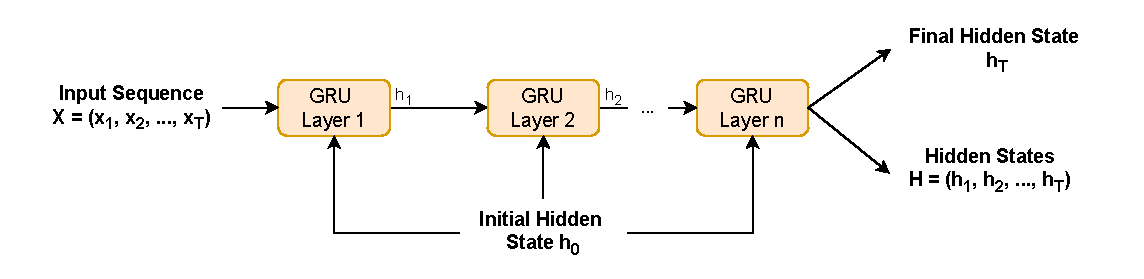
\includegraphics[width=1\textwidth]{figures/GRUSizPosEncoder.drawio.pdf}
    \caption{SizPos-GRU Encoder Architecture.}
    \label{fig:sizpos-gru-encoder}
\end{figure}

\subsubsection*{Position Encoder}
\noindent The position encoder processes the sequence of spatial dynamics vectors, which include the bounding box’s position, velocity, and acceleration over time. It is defined as:

\begin{equation}
    H_p, h_{p_T} = \text{GRU}_p(\mathbf{P}, h_{p_0}), \label{eq:position_encoder}
\end{equation}
Equation \eqref{eq:position_encoder} describes the position encoder, where $H_p$
is the sequence of hidden states generated by the GRU, and $h_{p_T}$ is the
final hidden state at time $T$.

\subsubsection*{Size Encoder}
\noindent The size encoder processes the sequence of dimensional attributes vectors, which include the bounding box’s width, height, and changes in these dimensions over time. It is defined as:

\begin{equation}
    H_d, h_{d_T} = \text{GRU}_d(\mathbf{D}, h_{d_0}), \label{eq:size_encoder}
\end{equation}
Equation \eqref{eq:size_encoder} outlines the size encoder, where $H_d$
represents the sequence of hidden states generated by the GRU, and $h_{d_T}$ is
the final hidden state at time $T$.

\subsection{Hidden State Fusion}
\noindent After the position and size encoders process their respective input sequences, the resulting hidden states are combined to leverage information from both spatial dynamics and dimensional attributes. This fusion is achieved by concatenating the final hidden states from both encoders and passing them through a fully connected layer:

\begin{equation}
    h_{\text{combined}} = W_{\text{combine}} \cdot \left[h_{p_T} \oplus h_{d_T}\right] + b_{\text{combine}}, \label{eq:hidden_state_fusion}
\end{equation}
As shown in Equation \eqref{eq:hidden_state_fusion}, the final hidden states from
the position and size encoders are concatenated and passed through a fully
connected layer to produce the fused hidden state $h_{\text{combined}}$. This
fused state encapsulates the temporal features from both input sequences,
enabling the model to generate context-aware predictions. 

\subsection{Decoders}
\noindent The \textit{SizPos-GRU} model utilises two specialised decoders to predict the future bounding boxes over the next \(m\) frames. These decoders are designed to process the temporal features extracted by the encoders and the fused hidden states, generating accurate and context-aware predictions. Figure~\ref{fig:sizpos-gru-decoder} illustrates the decoding process where the input sequence \( \mathbf{x}_t \) and the last hidden state \( h_{t-1} \) are processed through multiple GRU layers to generate the next hidden state \( h_t \). The sequence of hidden states \( H = \{h_1, h_2, \dots, h_t\} \) is then passed through a self-attention mechanism, which calculates attention scores and weights. The weighted sum of hidden states is combined with linear and non-linear transformations, including dropout and ReLU activation functions, to produce the final output \( \mathbf{x}_{t+1} \). This output is used for predicting the next time step in the sequence, continuing the process iteratively for future predictions.

\begin{figure}[H]
    \centering
    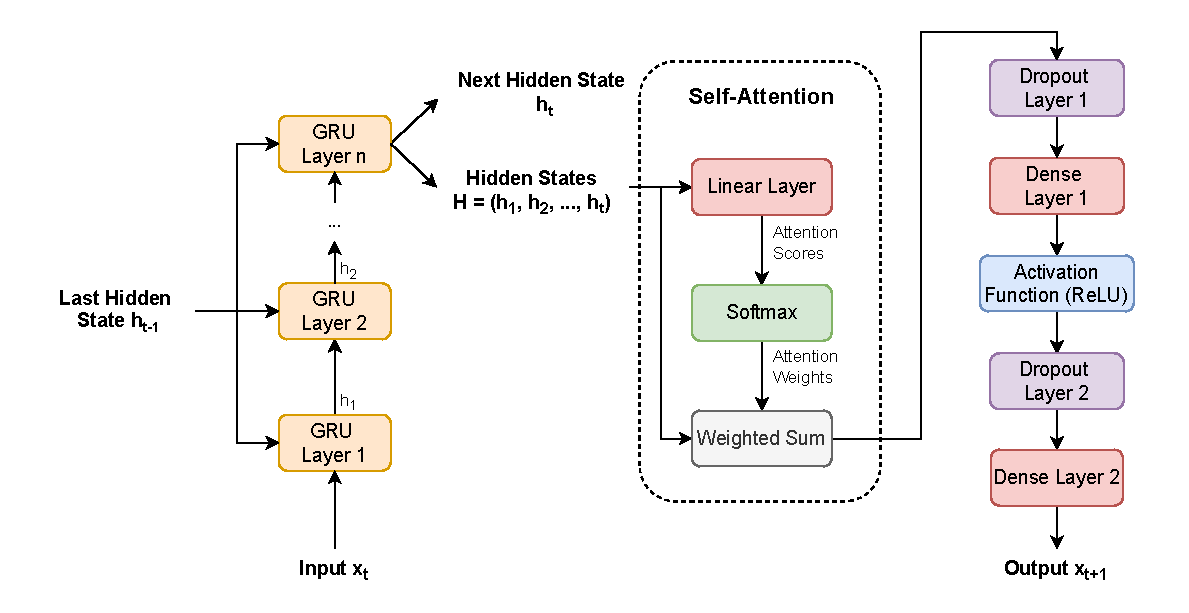
\includegraphics[width=1\textwidth]{figures/GRUSizPosDecoder.drawio.pdf}
    \caption{SizPos-GRU Decoder Architecture.}
    \label{fig:sizpos-gru-decoder}
\end{figure}

\subsubsection*{Position Decoder}
\noindent The position decoder is responsible for predicting the future spatial dynamics
of the bounding boxes, including their positions and velocities. The decoding
process begins by initialising the input with the last observed position in the
sequence. The decoder then iteratively predicts future positions over the
defined prediction horizon \(m\). During each iteration, the current input is
processed through a stack of GRU layers, which update the hidden state based on
the previous hidden state and current input. This updated hidden state,
encapsulating temporal dependencies, is then passed through a self-attention
mechanism. The self-attention mechanism computes attention scores, which are
normalised using a softmax function to produce attention weights. These weights
are applied to the hidden states to generate a context vector that highlights
the most relevant temporal features. The GRU layers within the position decoder
generate the sequence of hidden states \(H_p\) as shown in Equation
\eqref{eq:position_decoder_gru}, where \(H_p\) is derived from processing the
combined hidden states. The attention scores \(\alpha_i\) are calculated using
a linear transformation of each hidden state \(h_{p_i}\) (Equation
\eqref{eq:attention_scores_position}), and these scores are normalised to
produce the attention weights. The context vector \(c_p\) is then computed as
the weighted sum of the hidden states, as defined in Equation
\eqref{eq:context_vector_position}.

\begin{equation}
    H_p = \text{GRU}_p(h_{\text{combined}}), \label{eq:position_decoder_gru}
\end{equation}
\begin{equation}
    \alpha_i = \frac{\exp(w_i)}{\sum_{j=1}^{m}\exp(w_j)}, \quad w_i = \text{Linear}(h_{p_i}), \label{eq:attention_scores_position}
\end{equation}
\begin{equation}
    c_p = \sum_{i=1}^{m} \alpha_i h_{p_i}, \label{eq:context_vector_position}
\end{equation}
The context vector \(c_p\) is then passed through a series of fully connected
layers, with dropout and ReLU activation functions, to produce the final
position prediction for the current time step. The process is defined by
Equation \eqref{eq:position_prediction_1}, where the context vector is
transformed and refined through the network to generate the output prediction:

\begin{equation}
    \hat{\mathbf{P}}_{t+1:m} = \text{ReLU}(\text{Dropout}(\text{Dense}1(c_p))), \label{eq:position_prediction_1}
\end{equation}
\begin{equation}
    \hat{\mathbf{P}}_{t+1:m} = \text{Dense}2(\hat{\mathbf{P}}_{t+1:m}), \label{eq:position_prediction_2}
\end{equation}
As defined in Equation \eqref{eq:position_prediction_2}, the predicted position \(\hat{\mathbf{P}}_{t+1:m}\) is then used as the input
for the next iteration of the decoding loop, enabling the model to recursively
generate predictions for subsequent time steps. This iterative process
continues until predictions for all future time steps within the prediction
window have been generated, and the accumulated sequence of predicted positions
is returned as the final output.

\subsubsection*{Size Decoder}
\noindent The size decoder operates similarly to the position decoder but focuses on
predicting the future dimensions of the bounding boxes, such as width and
height. The decoding process starts with the last observed size in the
sequence, and the decoder iteratively generates predictions for future sizes
over the prediction horizon \(m\). In each iteration, the current size input is
processed through GRU layers that capture the temporal dynamics of size
changes. The output from the GRU is then passed through a self-attention
mechanism, which assigns different weights to the hidden states across time.
These weights are used to compute a context vector \(c_d\), which represents
the most relevant temporal and spatial information for the current prediction
step. The GRU layers within the size decoder generate the sequence of hidden
states \(H_d\) as shown in Equation \eqref{eq:size_decoder_gru}, where \(H_d\)
is derived from processing the combined hidden states. The attention scores
\(\beta_i\) are calculated using a linear transformation of each hidden state
\(h_{d_i}\) (Equation \eqref{eq:attention_scores_size}), and these scores are
normalised to produce the attention weights. The context vector \(c_d\) is then
computed as the weighted sum of the hidden states, as defined in Equation
\eqref{eq:context_vector_size}.

\begin{equation}
    H_d = \text{GRU}_d(h_{\text{combined}}), \label{eq:size_decoder_gru}
\end{equation}
\begin{equation}
    \beta_i = \frac{\exp(v_i)}{\sum_{j=1}^{m}\exp(v_j)}, \quad v_i = \text{Linear}(h_{d_i}), \label{eq:attention_scores_size}
\end{equation}
\begin{equation}
    c_d = \sum_{i=1}^{m} \beta_i h_{d_i}, \label{eq:context_vector_size}
\end{equation}
The context vector \(c_d\) is passed through dense layers with dropout and ReLU
activation to produce the final size prediction as shown in Equation
\eqref{eq:size_prediction_1}. The process refines the context vector through
transformations to generate the output prediction:

\begin{equation}
    \hat{\mathbf{D}}_{t+1:m} = \text{ReLU}(\text{Dropout}(\text{Dense}1(c_d))), \label{eq:size_prediction_1}
\end{equation}
\begin{equation}
    \hat{\mathbf{D}}_{t+1:m} = \text{Dense}2(\hat{\mathbf{D}}_{t+1:m}), \label{eq:size_prediction_2}
\end{equation}
Similar to the position decoder, the predicted size
\(\hat{\mathbf{D}}_{t+1:m}\) (Equation~\eqref{eq:size_prediction_2}) is then used as input for the next iteration,
ensuring that each prediction is contextually informed by previous outputs.
This loop continues until the decoder has generated predictions for all future
time steps within the prediction window \(m\), which are then returned as the
sequence of predicted sizes.

\section{Algorithm Design}

\subsection{Calculation of Key Values for Loss Functions}
\noindent In the \textit{SizPos-GRU} model, several values are calculated to derive the loss functions that guide the model training and optimisation process. These values are obtained by transforming the model's raw outputs into meaningful metrics that can be compared with the ground truth data. The key values calculated include:

\subsubsection*{Bounding Box and Velocity Estimation}
\noindent For each time step \(t\), the model predicts spatial dynamics \(\hat{\mathbf{p}}_t\) and dimensional attributes \(\hat{\mathbf{d}}_t\). These predictions are used to estimate bounding boxes and velocities, as shown in Equations \eqref{eq:bounding_box_x} to \eqref{eq:velocity_h}:

\begin{align}
    \hat{b}_{x,t} & = \hat{p}_{x,t},                    \label{eq:bounding_box_x} \\
    \hat{b}_{y,t} & = \hat{p}_{y,t},                    \label{eq:bounding_box_y} \\
    \hat{b}_{w,t} & = \hat{d}_{w,t},                    \label{eq:bounding_box_w} \\
    \hat{b}_{h,t} & = \hat{d}_{h,t},                    \label{eq:bounding_box_h} \\
    \hat{v}_{x,t} & = \hat{p}_{x,t} - \hat{p}_{x,t-1},  \label{eq:velocity_x}     \\
    \hat{v}_{y,t} & = \hat{p}_{y,t} - \hat{p}_{y,t-1},  \label{eq:velocity_y}     \\
    \hat{v}_{w,t} & = \hat{d}_{w,t} - \hat{d}_{w,t-1},  \label{eq:velocity_w}     \\
    \hat{v}_{h,t} & = \hat{d}_{h,t} - \hat{d}_{h,t-1}.  \label{eq:velocity_h}
\end{align}
Here, \(\hat{b}_{x,t}, \hat{b}_{y,t}, \hat{b}_{w,t}, \hat{b}_{h,t}\) represent
the predicted bounding box's center coordinates, width, and height at time
\(t\), and \(\hat{v}_{x,t}, \hat{v}_{y,t}, \hat{v}_{w,t}, \hat{v}_{h,t}\)
represent the corresponding velocities.

\subsubsection*{Velocity to Position Conversion}
\noindent To derive future positions from the predicted velocities, the following equations are used:

\begin{align}
    \hat{p}_{x,t+1} & = \hat{p}_{x,t} + \hat{v}_{x,t},  \label{eq:position_x} \\
    \hat{p}_{y,t+1} & = \hat{p}_{y,t} + \hat{v}_{y,t},  \label{eq:position_y} \\
    \hat{d}_{w,t+1} & = \hat{d}_{w,t} + \hat{v}_{w,t},  \label{eq:position_w} \\
    \hat{d}_{h,t+1} & = \hat{d}_{h,t} + \hat{v}_{h,t}.  \label{eq:position_h}
\end{align}
As indicated in Equations \eqref{eq:position_x} to \eqref{eq:position_h}, these
equations are used iteratively to predict the positions and sizes at each
future time step, integrating the model's output over time.

\newpage
\subsection{Loss Function Formulation}
To train the \textit{SizPos-GRU} model, Smooth L1 Loss, also known as Huber
Loss, a composite loss function is employed, which takes into account various
aspects of prediction accuracy. This loss function is a combination of L1 and
L2 losses, providing a balance between the two, making it less sensitive to
outliers than L2 loss while avoiding the large gradient changes associated with
L1 loss. The loss functions have been applied to various aspects of the model
predictions:

\subsubsection*{Size and Position Loss}
\noindent The model calculates the Smooth L1 Loss for the predicted sizes and positions compared to the ground truth data:

\begin{align}
    \mathcal{L}_{\text{size}}     & = \frac{1}{N} \sum_{t=1}^{m} \sum_{i \in \{w, h\}} \text{SmoothL1}\left(\hat{d}_{i,t}, d^{gt}_{i,t}\right),  \label{eq:size_loss}      \\
    \mathcal{L}_{\text{position}} & = \frac{1}{N} \sum_{t=1}^{m} \sum_{i \in \{x, y\}} \text{SmoothL1}\left(\hat{p}_{i,t}, p^{gt}_{i,t}\right).   \label{eq:position_loss}
\end{align}
Here, \(\mathcal{L}_{\text{size}}\) and \(\mathcal{L}_{\text{position}}\) are
the size and position loss functions, respectively, as shown in Equations
\eqref{eq:size_loss} and \eqref{eq:position_loss}, where \(\text{SmoothL1}(a,
b)\) is defined as:

\begin{equation}
    \text{SmoothL1}(a, b) =
    \begin{cases} 
        0.5 \times (a - b)^2 & \text{if } |a - b| < 1 \\ 
        |a - b| - 0.5        & \text{otherwise}.
    \end{cases} \label{eq:smooth_l1}
\end{equation}
Equation \eqref{eq:smooth_l1} defines the Smooth L1 function, which balances L1
and L2 loss characteristics to manage prediction errors.

\subsubsection*{Bounding Box Loss}
\noindent The model also computes the loss for the predicted bounding boxes, which represent the object's position and size in a unified format. The bounding box at each time step \(t\) is given by \(\hat{\mathbf{b}}_t = (\hat{b}_{x,t}, \hat{b}_{y,t}, \hat{b}_{w,t}, \hat{b}_{h,t})\). The loss for these predictions is calculated as:

\begin{equation}
    \mathcal{L}_{\text{bbox}} = \frac{1}{N} \sum_{t=1}^{m} \sum_{i \in \{x, y, w, h\}} \text{SmoothL1}\left(\hat{b}_{i,t}, b^{gt}_{i,t}\right), \label{eq:bbox_loss}
\end{equation}
where \(b^{gt}_{i,t}\) represents the ground truth bounding box coordinates and
dimensions at time \(t\), as shown in Equation \eqref{eq:bbox_loss}.

\subsubsection*{Velocity-to-Position Loss}
\noindent To ensure that the predicted velocities accurately translate to future positions, the model includes a loss term that compares the predicted positions derived from velocities (\(\hat{p}_{x,t+1}\), \(\hat{p}_{y,t+1}\), \(\hat{d}_{w,t+1}\), \(\hat{d}_{h,t+1}\)) with the ground truth positions and sizes at the next time step:

\begin{equation}
    \mathcal{L}_{\text{vel-to-pos}} = \frac{1}{N} \sum_{t=1}^{m} \sum_{i \in \{x, y, w, h\}} \text{SmoothL1}\left(\hat{p}_{i,t+1}, p^{gt}_{i,t+1}\right). \label{eq:vel_to_pos_loss}
\end{equation}

As defined in Equation \eqref{eq:vel_to_pos_loss}, this loss term ensures that
the model's predicted velocities are consistent with the subsequent positions,
reinforcing the temporal coherence of the predictions.

\subsubsection*{Total Loss}
\noindent The total loss used for model training is the sum of all the individual losses:

\begin{equation}
    \mathcal{L}_{\text{total}} = \mathcal{L}_{\text{size}} + \mathcal{L}_{\text{position}} + \mathcal{L}_{\text{bbox}} + \mathcal{L}_{\text{vel-to-pos}}. \label{eq:total_loss}
\end{equation}
Equation \eqref{eq:total_loss} defines the total loss function
\(\mathcal{L}_{\text{total}}\), which aggregates all loss components to guide
the training and optimisation process of the \textit{SizPos-GRU} model.

\subsection{Data Postprocessing}
Post-processing is a crucial step in the proposed prediction pipeline that
refines the raw predictions generated by the model. The main objective is to
enhance the accuracy and smoothness of the predicted bounding box trajectories
of the aircraft refuelling port. Several smoothing techniques are applied to
reduce noise and eliminate unrealistic variations in the predicted
trajectories. These techniques ensure that the final output is both accurate
and visually coherent.

\subsubsection*{Savitzky-Golay Filter}
\noindent The Savitzky-Golay filter is a digital filter used to smooth data while preserving its shape and features. It works by fitting successive subsets of data points with a low-degree polynomial. The filter is particularly effective in reducing noise without significantly distorting the signal. Given a trajectory $\mathbf{y} = \{y_1, y_2, \ldots, y_n\}$, the smoothed value at point $i$ is obtained by fitting a polynomial of degree $k$ over a window of size $2m + 1$ centered at $i$:

\begin{equation}
    \hat{y}_i = \sum_{j=-m}^{m} c_j y_{i+j}, \label{eq:savgol_filter}
\end{equation}
where $c_j$ are the coefficients determined by the polynomial fit, as shown in Equation \eqref{eq:savgol_filter}.

\subsubsection*{Moving Average Smoothing}
\noindent Moving average smoothing is a simple technique that calculates the average of a sliding window of data points, effectively reducing short-term fluctuations and highlighting longer-term trends. For a given trajectory $\mathbf{y}$, the smoothed value at point $i$ using a window of size $w$ is computed as:

\begin{equation}
    \hat{y}_i = \frac{1}{w} \sum_{j=0}^{w-1} y_{i-j}, \label{eq:moving_average}
\end{equation}
as indicated in Equation \eqref{eq:moving_average}. This method is straightforward and helps to smooth out irregularities in the trajectory.

\subsubsection*{Exponential Smoothing}
\noindent Exponential smoothing assigns exponentially decreasing weights to past observations, making it suitable for time-series data where recent data points are more relevant. The smoothed value at time $t$ is given by:

\begin{equation}
    \hat{y}_t = \alpha y_t + (1 - \alpha) \hat{y}_{t-1}, \label{eq:exponential_smoothing}
\end{equation}
where $\alpha$ is the smoothing factor, $0 < \alpha \leq 1$, and $\hat{y}_{t-1}$ is the previously smoothed value, as shown in Equation \eqref{eq:exponential_smoothing}.

\subsubsection*{Adaptive Smoothing}
\noindent Adaptive smoothing adjusts the degree of smoothing based on the variation observed in the data. If a significant change is detected between consecutive data points, more aggressive smoothing is applied. Given a trajectory $\mathbf{y}$, the adaptive smoothing is defined as:

\begin{equation}
    \hat{y}_t = 
    \begin{cases} 
        \text{Smooth}(\mathbf{y}_{t-k:t}) & \text{if } |y_t - y_{t-1}| > \text{threshold}, \\ 
        y_t                               & \text{otherwise},
    \end{cases} \label{eq:adaptive_smoothing}
\end{equation}
where $\text{Smooth}(\mathbf{y}_{t-k:t})$ applies a smoothing filter over the recent $k$ data points, as described in Equation \eqref{eq:adaptive_smoothing}.

\subsubsection*{Hybrid Smoothing}
\noindent Hybrid smoothing combines multiple smoothing techniques to leverage their strengths. Typically, a Savitzky-Golay filter is applied first, followed by a moving average smoothing on the already smoothed trajectory. Let $\hat{\mathbf{y}}^{(1)}$ be the output of the Savitzky-Golay filter applied to $\mathbf{y}$. The final smoothed trajectory $\hat{\mathbf{y}}^{(2)}$ is obtained by applying a moving average:

\begin{equation}
    \hat{\mathbf{y}}^{(2)} = \frac{1}{w} \sum_{j=0}^{w-1} \hat{y}^{(1)}_{i-j}, \label{eq:hybrid_smoothing}
\end{equation}
where $w$ is the window size for the moving average, as indicated in Equation \eqref{eq:hybrid_smoothing}.

\subsubsection*{Kalman Filter Smoothing}
\noindent The Kalman Filter is a statistical method used to estimate the state of a dynamic system from a series of noisy measurements. In our context, it is used to smooth the predicted bounding box trajectories by estimating the underlying motion parameters. The Kalman Filter operates in two main steps: prediction and update. The predicted state $\mathbf{x}_{t|t-1}$ and its covariance $\mathbf{P}_{t|t-1}$ are computed as:

\begin{equation}
    \mathbf{x}_{t|t-1} = \mathbf{F} \mathbf{x}_{t-1|t-1}, \label{eq:kalman_prediction_state}
\end{equation}
\begin{equation}
    \mathbf{P}_{t|t-1} = \mathbf{F} \mathbf{P}_{t-1|t-1} \mathbf{F}^T + \mathbf{Q}, \label{eq:kalman_prediction_covariance}
\end{equation}
where $\mathbf{F}$ is the state transition matrix, and $\mathbf{Q}$ is the process noise covariance matrix, as shown in Equations \eqref{eq:kalman_prediction_state} and \eqref{eq:kalman_prediction_covariance}. The update step corrects the prediction using the actual measurement $\mathbf{z}_t$:

\begin{equation}
    \mathbf{K}_t = \mathbf{P}_{t|t-1} \mathbf{H}^T (\mathbf{H} \mathbf{P}_{t|t-1} \mathbf{H}^T + \mathbf{R})^{-1}, \label{eq:kalman_gain}
\end{equation}
\begin{equation}
    \mathbf{x}_{t|t} = \mathbf{x}_{t|t-1} + \mathbf{K}_t (\mathbf{z}_t - \mathbf{H} \mathbf{x}_{t|t-1}), \label{eq:kalman_update_state}
\end{equation}
\begin{equation}
    \mathbf{P}_{t|t} = (\mathbf{I} - \mathbf{K}_t \mathbf{H}) \mathbf{P}_{t|t-1}, \label{eq:kalman_update_covariance}
\end{equation}
where $\mathbf{K}_t$ is the Kalman gain, $\mathbf{H}$ is the measurement matrix, and $\mathbf{R}$ is the measurement noise covariance, as defined in Equations \eqref{eq:kalman_gain} to \eqref{eq:kalman_update_covariance}.

%%%%%%%%%%%%%%%%%%%%%%%%%%%%%%%%%%%%%%%%%%%%%%%%%%%%%%%%%%%%%%%%%%%%%%%%%%%%%%%
%%%%%%%%%%%%%%%%%%%%%%%%%%%%% EXPERIMENT DESIGN %%%%%%%%%%%%%%%%%%%%%%%%%%%%%%%
\chapter{Experiment Design}\label{chap:experiment_design}
\section{Experiment Environment}
The experiments were conducted using a high-performance computing environment
optimised for deep learning tasks. The hardware configuration included an
NVIDIA A40 GPU with 48 GB of VRAM, 9 virtual CPUs (vCPUs), and 50 GB of RAM,
ensuring efficient handling of large-scale models and data processing tasks.
The software environment was based on a Linux operating system, utilising
PyTorch Lightning~\cite{Falcon_PyTorch_Lightning_2019} for sequence model
implementation. PyTorch Lightning provided a streamlined and modular framework,
improving experimentation and reproducibility. Data loading was managed using
PyTorch's \texttt{DataLoader}~\cite{Ansel_PyTorch_2_Faster_2024} with 8 worker
threads to maximise I/O efficiency. 

\section{Evaluation Metrics}
In order to assess the performance of the proposed framework for predicting the
future position of aircraft refuelling ports, it is imperative to utilise
appropriate evaluation metrics that reflect both the accuracy and reliability
of the predictions. This section outlines and discusses the four primary
evaluation metrics employed in this study: Average Displacement Error (ADE),
Final Displacement Error (FDE), Average Intersection over Union (AIoU), and
Final Intersection over Union (FIoU). These metrics provide a comprehensive
evaluation by measuring different aspects of the predicted trajectories and
bounding boxes.

\subsection*{Average Displacement Error (ADE)}
\noindent The Average Displacement Error (ADE) measures the average Euclidean distance between the predicted bounding box centers and the ground truth bounding box centers over all predicted frames. The ADE provides an overall measure of the spatial accuracy of the prediction model over time. It captures how closely the predicted trajectory follows the actual trajectory of the refuelling port. In practical terms, a lower ADE indicates that the model consistently predicts the position of the refuelling port with minimal deviation from its true path, which is critical in applications where continuous tracking and precise positioning are essential. It is defined as:

\begin{equation}
    \text{ADE} = \frac{1}{m} \sum_{t=1}^{m} \sqrt{(x_t^{\text{pred}} - x_t^{\text{gt}})^2 + (y_t^{\text{pred}} - y_t^{\text{gt}})^2}, \label{eq:ade}
\end{equation}
where \(m\) is the number of predicted frames, \((x_t^{\text{pred}},
y_t^{\text{pred}})\) represents the center of the predicted bounding box at the
\(t\)-th frame, and \((x_t^{\text{gt}}, y_t^{\text{gt}})\) represents the
center of the ground truth bounding box at the same frame. Equation
\eqref{eq:ade} shows that \(x_t^{\text{pred}}\), \(y_t^{\text{pred}}\),
\(x_t^{\text{gt}}\), \(y_t^{\text{gt}}\), and \(ADE\) are expressed in pixels.

\subsection*{Final Displacement Error (FDE)}
\noindent The Final Displacement Error (FDE) focuses on the accuracy of the predicted bounding box center in the final frame of the prediction horizon. The FDE is crucial for evaluating the model’s performance at the end of the prediction sequence. It focuses on the model’s ability to accurately predict the final position of the refuelling port. A lower FDE indicates a high level of precision in predicting the final position. It is defined as the Euclidean distance between the predicted and ground truth bounding box centers at the final frame \(T\):

\begin{equation}
    \text{FDE} = \sqrt{(x_T^{\text{pred}} - x_T^{\text{gt}})^2 + (y_T^{\text{pred}} - y_T^{\text{gt}})^2}. \label{eq:fde}
\end{equation}
As shown in Equation \eqref{eq:fde}, \((x_T^{\text{pred}}, y_T^{\text{pred}})\)
represents the center of the predicted bounding box at the final frame, and
\((x_T^{\text{gt}}, y_T^{\text{gt}})\) represents the center of the ground
truth bounding box at the same frame.

\subsection*{Average Intersection over Union (AIoU)}
\noindent The Average Intersection over Union (AIoU) evaluates the overlap between the predicted bounding boxes and the ground truth bounding boxes, averaged over all predicted frames. AIoU provides an integrated measure of both the spatial accuracy and the dimensional consistency of the predicted bounding boxes over time. A higher AIoU indicates that the predicted bounding boxes consistently maintain a high degree of overlap with the ground truth, reflecting the model’s ability to accurately track both the position and the scale of the refuelling port. This metric is particularly relevant in tasks where the object’s size and shape are critical, as it ensures that the detected object not only matches the position but also the correct dimensions, which is vital for the subsequent physical interaction with the object. It is computed as:

\begin{equation}
    \text{AIoU} = \frac{1}{m} \sum_{t=1}^{m} \frac{A(\mathbf{b}_t^{\text{pred}} \cap \mathbf{b}_t^{\text{gt}})}{A(\mathbf{b}_t^{\text{pred}} \cup \mathbf{b}_t^{\text{gt}})}, \label{eq:aiou}
\end{equation}
where \(A(\mathbf{b}_t^{\text{pred}} \cap \mathbf{b}_t^{\text{gt}})\) denotes
the area of the intersection between the predicted bounding box
\(\mathbf{b}_t^{\text{pred}}\) and the ground truth bounding box
\(\mathbf{b}_t^{\text{gt}}\) at the \(t\)-th frame, and
\(A(\mathbf{b}_t^{\text{pred}} \cup \mathbf{b}_t^{\text{gt}})\) denotes the
area of their union, as defined in Equation \eqref{eq:aiou}.

\subsection*{Final Intersection over Union (FIoU)}
\noindent The Final Intersection over Union (FIoU) assesses the overlap between the predicted bounding box and the ground truth bounding box at the final frame of the prediction horizon. FIoU is a critical metric when the final prediction accuracy is more important than the performance across all frames. It measures how well the predicted bounding box fits the ground truth at the crucial final moment, which is important for tasks that rely on the precise final positioning of an object. For instance, in automated systems that involve docking or alignment tasks, ensuring that the final predicted bounding box is highly accurate in terms of both position and size is essential for successful operation. A higher FIoU score implies a more reliable and accurate final prediction, which is indispensable in high-stakes applications where precision is paramount. It is defined as:

\begin{equation}
    \text{FIoU} = \frac{A(\mathbf{b}_T^{\text{pred}} \cap \mathbf{b}_T^{\text{gt}})}{A(\mathbf{b}_T^{\text{pred}} \cup \mathbf{b}_T^{\text{gt}})}, \label{eq:fiou}
\end{equation}
where \(A(\mathbf{b}_T^{\text{pred}} \cap \mathbf{b}_T^{\text{gt}})\) and
\(A(\mathbf{b}_T^{\text{pred}} \cup \mathbf{b}_T^{\text{gt}})\) denote the
intersection and union areas at the final frame \(m\), respectively, as shown
in Equation \eqref{eq:fiou}.

\section{Model Training and Optimisation}
\subsection*{Model Parameters}
\noindent The \textit{SizPos-GRU} model was trained using the Adam optimizer, which is
known for its ability to adapt learning rates for each parameter, enhancing the
convergence speed and stability of the training process~\cite{KingBa15,
    FusionGRU, DBLP:journals/corr/abs-2010-10270}. Adam computes adaptive learning
rates for each parameter by keeping track of both the first and second moments
of the gradients. This optimizer was selected due to its proven efficiency in
handling non-stationary objectives and noisy gradients, which are common in
deep learning models. The learning rate was dynamically adjusted using a
\textit{ReduceLROnPlateau} scheduler. This scheduler is particularly effective
in preventing the model from getting stuck in local minima by reducing the
learning rate when the validation loss stops improving~\cite{FusionGRU,
    DBLP:journals/corr/abs-2010-10270}. The learning rate
\(\text{LR}_{\text{new}}\) is updated according to the following rule:

\begin{equation}
    \text{LR}_{\text{new}} = \text{LR}_{\text{current}} \times \text{scheduler\_factor}, \label{eq:lr_update_rule}
\end{equation}
where \(\text{scheduler\_factor}\) is a predefined factor, typically set to a value less than 1, which controls how significantly the learning rate is reduced, as shown in Equation~\eqref{eq:lr_update_rule}. This approach allows the model to make finer updates as it converges, thereby improving the chances of finding a better local minimum. The training was conducted with close monitoring of validation performance to ensure the model's ability to generalize to unseen data. By using early stopping based on validation metrics, the training process was made more efficient, preventing overfitting and ensuring that the model retained its ability to perform well on new data. Tables~\ref{tab:training_parameters_description} and~\ref{tab:training_parameters_values} provide an overview of the training configuration parameters used for the \textit{SizPos-GRU} model. These parameters were selected based on the optimal results obtained from extensive hyperparameter tuning.

\begin{table}[H]
    \centering
    \caption{Training Configuration Parameters for the \textit{SizPos-GRU} model - Descriptions.}
    \label{tab:training_parameters_description}
    \begin{adjustbox}{max width=\textwidth}
        \begin{tabular}{lcc}
            \toprule
            \textbf{Parameter} & \textbf{Description}                                       \\ 
            \midrule
            Random Seed        & Seed value for reproducibility                             \\
            Number of Workers  & Number of CPU cores used for data loading                  \\
            Batch Size         & Number of samples per batch during training                \\
            Input Frames       & Number of input frames fed into the model                  \\
            Output Frames      & Number of frames predicted by the model                    \\
            Hidden Layer Size  & Size of the hidden layers in the GRU network               \\
            Number of Layers   & Number of GRU layers stacked in the network                \\
            Learning Rate      & Initial learning rate for the optimizer                    \\
            Scheduler Patience & Number of epochs to wait before reducing the learning rate \\
            Scheduler Factor   & Factor by which the learning rate is reduced               \\
            Max Epochs         & Maximum number of epochs for training                      \\
            Dropout Rate       & Probability of dropping a neuron during training           \\
            Optimizer          & Optimisation algorithm used for training                   \\
            Scheduler          & Learning rate scheduler used for dynamic adjustment        \\
            Checkpoint Metric  & Metric used to save the best model checkpoint              \\
            \bottomrule
        \end{tabular}
    \end{adjustbox}
\end{table}

\begin{table}[H]
    \centering
    \caption{Training Configuration Parameters for the \textit{SizPos-GRU} model - Values.}
    \label{tab:training_parameters_values}
    \begin{adjustbox}{max width=\textwidth}
        \begin{tabular}{lcc}
            \toprule
            \textbf{Parameter} & \textbf{1 sec Prediction (30 frames)} & \textbf{2 sec Prediction (60 frames)} \\ 
            \midrule
            Random Seed        & 42                                    & 42                                    \\
            Number of Workers  & 8                                     & 8                                     \\
            Batch Size         & 64                                    & 64                                    \\
            Input Frames       & 15                                    & 30                                    \\
            Output Frames      & 30                                    & 60                                    \\
            Hidden Layer Size  & 256                                   & 128                                   \\
            Number of Layers   & 8                                     & 8                                     \\
            Learning Rate      & $5 \times 10^{-4}$                    & $5 \times 10^{-4}$                    \\
            Scheduler Patience & 10 epochs                             & 10 epochs                             \\
            Scheduler Factor   & 0.9                                   & 0.9                                   \\
            Max Epochs         & 100                                   & 100                                   \\
            Dropout Rate       & 0.2                                   & 0.2                                   \\
            Optimizer          & Adam                                  & Adam                                  \\
            Scheduler          & ReduceLROnPlateau                     & ReduceLROnPlateau                     \\
            Checkpoint Metric  & Best Final FDE                        & Best Final FDE                        \\
            \bottomrule
        \end{tabular}
    \end{adjustbox}
\end{table}

\newpage
\subsection*{Hyperparameter Tuning}
\noindent Extensive hyperparameter tuning was conducted to determine the most effective
configurations for the \textit{SizPos-GRU} model. This process involved systematically
varying key parameters to assess their impact on model performance. The goal
was to strike a balance between model complexity and computational efficiency
while ensuring that the model could learn effectively from the available data.
Tables~\ref{tab:hp_tuning_descriptions} and~\ref{tab:hp_tuning_values} summarise the hyperparameter tuning configuration,
listing the range of values tested for each parameter. The tuning process
included exploring different sizes and numbers of hidden layers, varying the
number of input and output frames, and adjusting the learning rate, among other
factors.

\begin{table}[H]
    \centering
    \caption{Hyperparameter Tuning Configuration - Descriptions}
    \label{tab:hp_tuning_descriptions}
    \begin{adjustbox}{max width=\textwidth}
        \begin{tabular}{lcc}
            \toprule
            \textbf{Parameter}      & \textbf{Description}                         \\ 
            \midrule
            Input Frames            & Number of input frames fed into the model    \\ 
            Output Frames           & Number of frames predicted by the model      \\ 
            Hidden Layer Sizes      & Size of the hidden layers in the GRU network \\ 
            Number of Hidden Layers & Number of GRU layers stacked in the network  \\ 
            \bottomrule
        \end{tabular}
    \end{adjustbox}
\end{table}

\begin{table}[H]
    \centering
    \caption{Hyperparameter Tuning Configuration - Values Tested}
    \label{tab:hp_tuning_values}
    \begin{adjustbox}{max width=\textwidth}
        \begin{tabular}{lcc}
            \toprule
            \textbf{Parameter}      & \textbf{Values Tested} \\ 
            \midrule
            Input Frames            & 15, 30                 \\ 
            Output Frames           & 30, 60                 \\ 
            Hidden Layer Sizes      & 32, 64, 128, 256, 512  \\ 
            Number of Hidden Layers & 1, 2, 4, 8             \\ 
            \bottomrule
        \end{tabular}
    \end{adjustbox}
\end{table}

\noindent The final selection of hyperparameters, informed by the tuning results, was
critical in ensuring the \textit{SizPos-GRU} model's effectiveness. The chosen
parameters provided a balance that allowed the model to perform well across
different scenarios while maintaining computational efficiency. This careful
calibration was essential for achieving the desired model accuracy and
robustness during the training process.

\subsection*{Data Augmentation Strategy}
\noindent The data augmentation strategy is designed to enhance the model's robustness
and generalization capability by simulating various camera movements and
imperfections that might occur in real-world scenarios. This approach ensures
the model is well-prepared to handle diverse and unpredictable situations. The augmentation strategy is applied with several considerations to maintain
data integrity and ensure realistic training conditions. Augmentations are
exclusively applied during the training stage to avoid influencing evaluation
results, ensuring that the model's performance is assessed on clean,
unaugmented data. Each sequence has a 50\% probability of being augmented,
which ensures a balanced mix of original and augmented data. This probabilistic
approach prevents overfitting to any single type of augmentation. When
augmentations are applied, they affect both input and output sequences
consistently, maintaining temporal coherence and realism across the sequence,
which is crucial for models learning from sequential data. All augmented values
are clipped to the range [0, 1], ensuring they remain valid normalised
coordinates in the YOLO format. This clipping ensures that the augmented
bounding boxes are usable within the model's expected input format. The data
loading process also includes error handling mechanisms to manage any
inconsistencies in the data, ensuring that training can continue even if
individual samples are problematic.

\subsubsection*{Sequence Reversal}
\noindent To effectively double the size of the training dataset, reversed sequences are
included. For each original sequence $(S_1, S_2, \ldots, S_n)$, a corresponding
reversed sequence $(S_n, S_{n-1}, \ldots, S_1)$ is added. This augmentation
enables the model to learn to predict both forward and backward camera
movements relative to the aircraft refuelling port, thereby enhancing its
adaptability.

\subsubsection*{Camera Movement Simulation}
\noindent Subtle camera movements are simulated to improve the model's robustness to
varying camera positions. Panning is applied by introducing a smooth,
cumulative random offset to the x and y coordinates of the bounding boxes,
simulating the effect of the camera panning horizontally or vertically. The
panning effect is modeled as:
\[
    \text{pan}_t = \sum_{i=1}^t \frac{N(0, \sigma^2)}{5}
\]
where $N(0, \sigma^2)$ represents a normal distribution with a mean of 0 and
variance $\sigma^2$. This simulation ensures the model can effectively handle
gradual shifts in the camera's viewpoint.

\subsubsection*{Zoom Simulation}

\noindent To account for changes in the apparent size of the refuelling port due to camera
zoom or aircraft movement, a smooth, cumulative scaling factor is applied to
the width and height of the bounding boxes. The zoom effect is modeled as:
\[
    \text{zoom}_t = \prod_{i=1}^t U(0.98, 1.02)
\]
where $U(0.98, 1.02)$ is a uniform distribution between 0.98 and 1.02. This
augmentation prepares the model to adapt to scenarios where the distance
between the camera and the refuelling port changes dynamically.

\subsubsection*{Detection Inaccuracy Simulation}

\noindent To enhance the model's resilience to slight inaccuracies in object detection,
small Gaussian noise is added to all bounding box coordinates. This noise is
sampled from $N(0, 0.002^2)$ for each coordinate, introducing minor variations
that simulate real-world detection imperfections. Such noise mimics the slight
inaccuracies that can occur in detection algorithms due to environmental
factors or sensor noise.

\newpage
\section{Comparison Experiments}
To evaluate the performance of the proposed \textit{SizPos-GRU} model, a series
of comparison experiments were conducted using several baseline models. These
experiments are designed to assess the model's capability in predicting the
future positions and sizes of the refuelling port in video sequences. The
baseline models considered include the Linear Kalman Filter (LKF), Constant
Velocity (CV) model, and variants of Recurrent Neural Networks (RNNs) such as
Long Short-Term Memory (LSTM) and Gated Recurrent Unit (GRU).

\subsection*{Linear Kalman Filter (LKF)}
\noindent The Linear Kalman Filter (LKF) is a recursive filter that estimates the state of a linear dynamic system from a series of incomplete and noisy measurements. In the context of predicting the position of the refuelling port, the state vector $\mathbf{x}_t$ includes the position and velocity of the object. The model assumes constant velocity in the state transition, which is represented mathematically by the following equation:

\begin{equation}
    \mathbf{x}_t = \mathbf{F} \mathbf{x}_{t-1} + \mathbf{w}_{t-1}, \label{eq:kalman_state_transition}
\end{equation}
In Equation \eqref{eq:kalman_state_transition}, $\mathbf{F}$ is the state transition matrix that models how the state evolves from time $t-1$ to $t$, and $\mathbf{w}_{t-1}$ is the process noise, which accounts for any uncertainty in the system dynamics. The Kalman Filter also relies on an observation model to relate the state
vector $\mathbf{x}_t$ to the actual measurements $\mathbf{z}_t$. This
relationship is expressed as:

\begin{equation}
    \mathbf{z}_t = \mathbf{H} \mathbf{x}_t + \mathbf{v}_t, \label{eq:kalman_observation}
\end{equation}
Here, in Equation \eqref{kalman_observation}, $\mathbf{H}$ is the observation matrix, which maps the true state space into the observed space, and $\mathbf{v}_t$ represents the measurement noise, capturing the inaccuracies in the sensor data.
The Kalman Filter proceeds with two main steps: prediction and update. During
the prediction step, the filter estimates the current state and its covariance
based on the previous state:

\begin{align}
    \hat{\mathbf{x}}_{t|t-1} & = \mathbf{F} \hat{\mathbf{x}}_{t-1|t-1}, \label{eq:kalman_prediction_step_state}                             \\
    \mathbf{P}_{t|t-1}       & = \mathbf{F} \mathbf{P}_{t-1|t-1} \mathbf{F}^\top + \mathbf{Q}, \label{eq:kalman_prediction_step_covariance}
\end{align}
In Equation~\eqref{eq:kalman_prediction_step_state}, $\hat{\mathbf{x}}_{t|t-1}$ denotes the predicted state at time $t$ based on the state at time $t-1$, and $\mathbf{P}_{t|t-1}$ in Equation~\eqref{eq:kalman_prediction_step_covariance} represents the predicted covariance matrix, which quantifies the uncertainty in the predicted state. The matrix $\mathbf{Q}$ is the process noise covariance, reflecting the uncertainty in the system's evolution.
In the update step, the filter adjusts the predicted state and covariance using
the actual measurement $\mathbf{z}_t$ obtained at time $t$:

\begin{align}
    \mathbf{K}_t           & = \mathbf{P}_{t|t-1} \mathbf{H}^\top \left(\mathbf{H} \mathbf{P}_{t|t-1} \mathbf{H}^\top + \mathbf{R}\right)^{-1}, \label{eq:kalman_update_step_gain} \\
    \hat{\mathbf{x}}_{t|t} & = \hat{\mathbf{x}}_{t|t-1} + \mathbf{K}_t \left(\mathbf{z}_t - \mathbf{H} \hat{\mathbf{x}}_{t|t-1}\right), \label{eq:kalman_update_step_state}        \\
    \mathbf{P}_{t|t}       & = \left(\mathbf{I} - \mathbf{K}_t \mathbf{H}\right) \mathbf{P}_{t|t-1}. \label{eq:kalman_update_step_covariance}
\end{align}
In Equation~\eqref{eq:kalman_update_step_gain}, $\mathbf{K}_t$ is the Kalman gain, which determines the weight given to the new measurement versus the predicted state. The updated state estimate $\hat{\mathbf{x}}_{t|t}$ in Equation~\eqref{eq:kalman_update_step_state} is computed by correcting the predicted state $\hat{\mathbf{x}}_{t|t-1}$ with the measurement innovation (the difference between the actual and predicted measurements). Finally, the updated covariance $\mathbf{P}_{t|t}$, as shown in Equation~\eqref{eq:kalman_update_step_covariance}, reflects the uncertainty in the updated state, incorporating the reduction in uncertainty achieved through the measurement update.
The Kalman Filter iteratively performs these prediction and update steps,
optimally combining prior knowledge and new measurements to provide a refined
estimate of the refuelling port's position and velocity over time.

\subsection*{Constant Velocity (CV)}
\noindent The Constant Velocity (CV) model assumes that the object continues to move at a constant speed and direction. This model is based on the principle that the object's motion remains uniform over time. Given a sequence of past positions $\mathbf{P} = \{(x_1, y_1), \dots, (x_T, y_T)\}$, the model first estimates the velocity $\mathbf{v}$ of the object. This velocity is computed by averaging the differences between consecutive positions:

\begin{equation}
    \mathbf{v} = \frac{1}{T-1} \sum_{t=2}^{T} \left(\mathbf{P}_t - \mathbf{P}_{t-1}\right), \label{eq:cv_velocity}
\end{equation}
In Equation~\eqref{eq:cv_velocity}, $\mathbf{v}$ represents the average velocity, calculated over $T-1$ time steps, where $\mathbf{P}_t$ is the position at time $t$ and $\mathbf{P}_{t-1}$ is the position at the previous time step. This average velocity assumes that the object has moved at a constant speed between each pair of consecutive positions.
Once the velocity $\mathbf{v}$ is determined, the future positions
$\mathbf{F}_{k}$ for $k$ future steps can be predicted using the following
equation:

\begin{equation}
    \mathbf{F}_k = \mathbf{P}_T + k \cdot \mathbf{v}, \label{eq:cv_future_positions}
\end{equation}
In Equation~\eqref{eq:cv_future_positions}, $\mathbf{F}_k$ represents the predicted position of the object after $k$ future time steps. The prediction is made by linearly extrapolating from the last observed position $\mathbf{P}_T$, with the object's position adjusted by the product of the velocity $\mathbf{v}$ and the number of time steps $k$ into the future. This approach is straightforward and computationally efficient, making it
useful for quick predictions in scenarios where the motion is relatively
simple. However, its simplicity also means that it may be limited in handling
more complex, dynamic, or non-linear motions, where the assumption of constant
velocity does not hold true.

\newpage
\subsection*{LSTM Model (PosVelAcc-LSTM)}
\noindent The PosVelAcc-LSTM model leverages Long Short-Term Memory (LSTM) networks to predict future bounding box positions by encoding past positions, velocities, and accelerations. The model architecture is designed to capture the temporal dependencies in these input sequences, allowing for more accurate predictions of future movements. The architecture includes separate LSTM encoders for each input sequence (positions, velocities, and accelerations) and corresponding decoders for generating the predicted positions and velocities. This model was inspired by the PV-LSTM model from~\citet{DBLP:journals/corr/abs-2010-10270}. The following algorithm outlines the process of the PosVelAcc-LSTM model:

\begin{algorithm}[H]
    \caption{PosVelAcc-LSTM Model}\label{alg:lstm_posvelacc}
    \begin{algorithmic}[1]
        \Require $\mathbf{P}$ (position sequence), $\mathbf{V}$ (velocity sequence), $\mathbf{A}$ (acceleration sequence)
        \State Encode past positions, velocities, and accelerations using LSTM encoders
        \State Combine encoded states: $\mathbf{h}_{\text{combined}} = \mathbf{h}_P + \mathbf{h}_V + \mathbf{h}_A$
        \State Initialise decoder inputs with the last observed position and velocity
        \For{$t = 1$ to $k$} \Comment{Predict for $k$ future steps}
        \State Predict future position: $\hat{\mathbf{P}}_{t+1} = \text{LSTMDecoder}(\mathbf{h}_{\text{combined}})$
        \State Predict future velocity: $\hat{\mathbf{V}}_{t+1} = \text{LSTMDecoder}(\mathbf{h}_{\text{combined}})$
        \EndFor
        \State \Return Predicted positions and velocities
    \end{algorithmic}
\end{algorithm}

\noindent The model begins by encoding the sequences of past positions, velocities, and accelerations using separate LSTM encoders. The resulting hidden states $\mathbf{h}_P$, $\mathbf{h}_V$, and $\mathbf{h}_A$ are then combined into a unified representation $\mathbf{h}_{\text{combined}}$, which captures the joint temporal dependencies of these three input sequences.
The decoding process starts with initialising the decoder inputs using the last observed position and velocity. For each future time step $t$ (up to $k$ steps), the model predicts the future position $\hat{\mathbf{P}}_{t+1}$ and velocity $\hat{\mathbf{V}}_{t+1}$ using the LSTM decoders, as shown in the algorithm.
The training of the PosVelAcc-LSTM model is guided by minimising a composite loss function, which includes terms for both position and velocity predictions. This loss function is given by:

\begin{equation}
    \mathcal{L}_{\text{total}} = \text{SmoothL1}(\hat{\mathbf{P}}, \mathbf{P}_{\text{true}}) + \text{SmoothL1}(\hat{\mathbf{V}}, \mathbf{V}_{\text{true}}), \label{eq:posvelacc_lstm_loss}
\end{equation}
\noindent In Equation~\eqref{eq:posvelacc_lstm_loss}, $\hat{\mathbf{P}}$ and $\hat{\mathbf{V}}$ represent the predicted positions and velocities, respectively, while $\mathbf{P}_{\text{true}}$ and $\mathbf{V}_{\text{true}}$ represent the corresponding ground truth values. The loss function uses the Smooth L1 loss (also known as Huber loss), which is robust to outliers and provides a balance between the L1 and L2 loss characteristics. By minimising $\mathcal{L}_{\text{total}}$, the model learns to accurately predict both the positions and velocities over the future time steps.

\newpage
\subsection*{LSTM Model (SizPos-LSTM)}
\noindent The SizPos-LSTM model extends the traditional LSTM architecture to predict both future bounding box positions and sizes. This model is specifically designed to handle two separate input sequences: the sequence of bounding box positions and the sequence of bounding box sizes. To achieve this, the model includes separate LSTM encoders for each type of sequence and corresponding decoders that predict future positions and sizes. The overall process of the SizPos-LSTM model can be outlined as follows:

\begin{algorithm}[H]
    \caption{SizPos-LSTM Model}\label{alg:lstm_sizpos}
    \begin{algorithmic}[1]
        \Require $\mathbf{P}$ (position sequence), $\mathbf{S}$ (size sequence)
        \State Encode position and size using LSTM encoders
        \State Combine encoded states: $\mathbf{h}_{\text{combined}} = \text{Combine}(\mathbf{h}_P, \mathbf{h}_S)$
        \State Initialise decoder inputs with the last observed position and size
        \For{$t = 1$ to $k$} \Comment{Predict for $k$ future steps}
        \State Predict future position: $\hat{\mathbf{P}}_{t+1} = \text{LSTMDecoder}(\mathbf{h}_{\text{combined}})$
        \State Predict future size: $\hat{\mathbf{S}}_{t+1} = \text{LSTMDecoder}(\mathbf{h}_{\text{combined}})$
        \EndFor
        \State \Return Predicted positions and sizes
    \end{algorithmic}
\end{algorithm}

\noindent The model begins by encoding the position sequence $\mathbf{P}$ and the size sequence $\mathbf{S}$ using separate LSTM encoders. The encoded hidden states, denoted as $\mathbf{h}_P$ for positions and $\mathbf{h}_S$ for sizes, are then combined into a unified representation $\mathbf{h}_{\text{combined}}$. This combined hidden state captures the temporal dependencies in both the positional and dimensional aspects of the bounding boxes.
In the decoding phase, the model initialises the decoder inputs using the last
observed position and size. It then iteratively predicts the future positions
$\hat{\mathbf{P}}_{t+1}$ and sizes $\hat{\mathbf{S}}_{t+1}$ for each future
time step $t$ up to $k$ steps, using the combined hidden state
$\mathbf{h}_{\text{combined}}$. The training process for the SizPos-LSTM model involves minimising a composite
loss function that includes terms for both position and size predictions. This
loss function is expressed as:

\begin{equation}
    \mathcal{L}_{\text{total}} = \text{SmoothL1}(\hat{\mathbf{P}}, \mathbf{P}_{\text{true}}) + \text{SmoothL1}(\hat{\mathbf{S}}, \mathbf{S}_{\text{true}}), \label{eq:sizpos_lstm_loss}
\end{equation}
In Equation~\eqref{eq:sizpos_lstm_loss}, $\hat{\mathbf{P}}$ and $\hat{\mathbf{S}}$ represent the predicted positions and sizes, respectively, while $\mathbf{P}_{\text{true}}$ and $\mathbf{S}_{\text{true}}$ represent the corresponding ground truth values. The loss function uses the Smooth L1 loss (also known as Huber loss), which balances sensitivity to outliers with the need to minimize large deviations. This composite loss $\mathcal{L}_{\text{total}}$ ensures that the model learns to accurately predict both the positions and sizes of bounding boxes over future time steps.

\newpage
\subsection*{GRU Model (PosVelAcc)}
\noindent The PosVelAcc-GRU model is similar to the PosVelAcc-LSTM model, but it utilises a Gated Recurrent Unit (GRU) network instead of LSTM for both encoding and decoding. GRUs are known for offering computational efficiency while maintaining the ability to capture temporal dependencies effectively, making them a suitable choice for sequence prediction tasks. This model is inspired by the Fusion-GRU model from~\citet{FusionGRU}. The GRU model operates with the following key components:

\begin{align}
    \mathbf{z}_t         & = \sigma(\mathbf{W}_z \mathbf{x}_t + \mathbf{U}_z \mathbf{h}_{t-1}), \label{eq:gru_update_gate}                                    \\
    \mathbf{r}_t         & = \sigma(\mathbf{W}_r \mathbf{x}_t + \mathbf{U}_r \mathbf{h}_{t-1}), \label{eq:gru_reset_gate}                                     \\
    \mathbf{\tilde{h}}_t & = \text{tanh}(\mathbf{W}_h \mathbf{x}_t + \mathbf{r}_t \odot \mathbf{U}_h \mathbf{h}_{t-1}), \label{eq:gru_candidate_hidden_state} \\
    \mathbf{h}_t         & = (1 - \mathbf{z}_t) \odot \mathbf{h}_{t-1} + \mathbf{z}_t \odot \mathbf{\tilde{h}}_t, \label{eq:gru_hidden_state}
\end{align}

\noindent The update gate $\mathbf{z}_t$, as defined in Equation~\eqref{eq:gru_update_gate}, controls the degree to which the previous hidden state $\mathbf{h}_{t-1}$ contributes to the current hidden state $\mathbf{h}_t$. This gate helps the model to decide how much past information should be passed forward to the next time step.
The reset gate $\mathbf{r}_t$, shown in Equation~\eqref{eq:gru_reset_gate}, determines how much of the past information to forget. This gate is crucial in allowing the model to reset its memory selectively, enabling it to capture more complex temporal patterns.
The candidate hidden state $\mathbf{\tilde{h}}_t$, calculated in Equation~\eqref{eq:gru_candidate_hidden_state}, represents the potential value for the new hidden state based on the current input $\mathbf{x}_t$ and the previous hidden state $\mathbf{h}_{t-1}$, modulated by the reset gate.
Finally, the hidden state $\mathbf{h}_t$ at time $t$, given by Equation~\eqref{eq:gru_hidden_state}, is a linear interpolation between the previous hidden state $\mathbf{h}_{t-1}$ and the candidate hidden state $\mathbf{\tilde{h}}_t$, with the weights determined by the update gate $\mathbf{z}_t$. This final hidden state $\mathbf{h}_t$ encapsulates the temporal dependencies and is used in the decoding process to predict future positions and velocities.
The PosVelAcc-GRU model leverages these mechanisms to efficiently process sequences of past positions, velocities, and accelerations, making it capable of generating accurate predictions for future bounding box positions and velocities while being computationally efficient.

\newpage
\section{Framework Evaluation}

This framework integrates YOLOv10 for object detection and the
\textit{SizPos-GRU} model for future position prediction. The process begins by
performing object detection across all frames of a video to establish ground
truth for each frame. This pre-obtained ground truth simplifies the subsequent
evaluation of prediction accuracy. The framework operates in a loop, where it
first detects objects in 15 frames, then predicts their positions over the next
30 frames using the \textit{SizPos-GRU} model. After each prediction phase, the
next 15 frames are analysed for new detections, and this cycle repeats. By
having the ground truth available from the outset, the framework allows for
efficient evaluation of predictions, directly comparing predicted positions
with known ground truth. The following pseudocode outlines the key steps of the
framework:

\begin{algorithm}[H]
    \caption{Object Detection and Future Position Prediction Framework}
    \label{alg:framework}
    \begin{algorithmic}[1]
        \Procedure{RunFramework}{$input\_video\_path$, $yolo\_weights\_path$, $gru\_model\_path$, $hparams\_file$, $output\_video\_path$, $output\_json\_path$, $smoothing\_filter$, $lkf$, $input\_frames$, $future\_frames$}

        \State Load YOLOv10 model with $yolo\_weights\_path$
        \State Open video file at $input\_video\_path$

        \State $detections \gets []$
        \While{frames in video}
        \State $frame \gets $ Read next frame
        \State $results \gets $ YOLOv10.detect($frame$)
        \State $detections \gets $ Extract bounding boxes from $results$
        \EndWhile

        \State Store $detections$ as ground truth for all frames

        \State Initialise loop to process detections in segments

        \While{more detections to process}
        \State $segment\_detections \gets $ Take next $input\_frames$ from $detections$
        \State $track\_history\_bbox \gets $ Update with $segment\_detections$

        \If{$track\_history\_bbox$ is full}
        \State $predicted\_positions \gets $ GRU.predict($track\_history\_bbox$)
        \If{$lkf$ is True}
        \State $predicted\_positions \gets $ Apply Kalman Filter to $predicted\_positions$
        \EndIf

        \State $smoothed\_combined\_bboxes \gets $ Apply chosen $smoothing\_filter$ to $predicted\_positions$

        \For{each future frame in $future\_frames$}
        \State Calculate prediction metrics (e.g., ADE, FDE, IoU)
        \State Annotate frame with current, predicted, and ground-truth bounding boxes
        \EndFor
        \EndIf

        \State Continue to next $input\_frames$ in $detections$
        \EndWhile

        \State Save annotated video to $output\_video\_path$
        \State Save prediction metrics and smoothed detections to $output\_json\_path$

        \EndProcedure
    \end{algorithmic}
\end{algorithm}

%%%%%%%%%%%%%%%%%%%%%%%%%%%%%%%%%%%%%%%%%%%%%%%%%%%%%%%%%%%%%%%%%%%%%%%%%%%%%%%
%%%%%%%%%%%%%%%%%%%%%%%%%%%% RESULTS & DISCUSSION %%%%%%%%%%%%%%%%%%%%%%%%%%%%%
\chapter{Results and Discussion}\label{chap:results}

\section{Object Detection Training Results}

This section presents the final testing results of three different YOLO
models—YOLOv10n.pt, YOLOv10s.pt, and YOLOv10m.pt—on a dataset focused on
classifying fuel port states (CLOSED, SEMI-OPEN, OPEN). The evaluation
considers key performance metrics, including Precision (P), Recall (R), mean
Average Precision at 50\% IoU (mAP50), and mean Average Precision across
multiple IoU thresholds (mAP50-95).

\begin{table}[H]
    \centering
    \caption{Performance comparison of finetuned YOLO models on the detection of Refueling Port.}
    \begin{adjustbox}{max width=\textwidth}
        \begin{tabular}{lcccccc}
            \toprule
            \textbf{Model}                        & \textbf{Metric} & \textbf{All}   & \textbf{Fuel Port [CLOSED]} & \textbf{Fuel Port [SEMI-OPEN]} & \textbf{Fuel Port [OPEN]} \\
            \midrule
            \multirow{4}{*}{\textbf{YOLOv10n.pt}} & Precision (P)   & 0.989          & 0.994                       & 0.982                          & \textbf{0.992}            \\
                                                  & Recall (R)      & 0.876          & 0.657                       & 0.996                          & 0.974                     \\
                                                  & mAP50           & \textbf{0.893} & 0.696                       & 0.995                          & 0.987                     \\
                                                  & mAP50-95        & \textbf{0.852} & 0.684                       & 0.962                          & \textbf{0.909}            \\
            \midrule
            \multirow{4}{*}{\textbf{YOLOv10s.pt}} & Precision (P)   & \textbf{0.997} & \textbf{0.998}              & \textbf{1.000}                 & \textbf{0.992}            \\
                                                  & Recall (R)      & 0.884          & \textbf{0.682}              & 0.997                          & 0.974                     \\
                                                  & mAP50           & \textbf{0.893} & 0.694                       & \textbf{0.995}                 & \textbf{0.989}            \\
                                                  & mAP50-95        & 0.848          & 0.678                       & 0.961                          & 0.905                     \\
            \midrule
            \multirow{4}{*}{\textbf{YOLOv10m.pt}} & Precision (P)   & 0.994          & 0.996                       & 0.999                          & 0.988                     \\
                                                  & Recall (R)      & \textbf{0.888} & \textbf{0.682}              & \textbf{1.000}                 & \textbf{0.983}            \\
                                                  & mAP50           & 0.892          & \textbf{0.701}              & \textbf{0.995}                 & 0.981                     \\
                                                  & mAP50-95        & \textbf{0.852} & \textbf{0.692}              & \textbf{0.968}                 & 0.897                     \\
            \bottomrule
        \end{tabular}
    \end{adjustbox}
    \label{tab:comparison}
\end{table}

\noindent The object detection performance of the three YOLO models was evaluated based
on their ability to detect the aircraft refuelling port in its different
states: CLOSED, SEMI-OPEN, and OPEN. Table~\ref{tab:comparison} provides a
comprehensive comparison across various metrics, with certain values
highlighted in bold to signify the best performance for each specific metric
across the models. The bold values in the table indicate the highest scores
within each metric category, either across all states or within specific fuel
port states. These bold values highlight the model that performed the best for
that particular metric (Precision, Recall, mAP50, mAP50-95) in the
corresponding category (All, CLOSED, SEMI-OPEN, OPEN). The comparison is made
on a row-by-row basis. For each row representing a specific performance metric,
the values are compared across the three models (YOLOv10n.pt, YOLOv10s.pt,
YOLOv10m.pt). For instance,
YOLOv10s.pt exhibited the highest precision overall at 0.997, as well as the
highest precision across all fuel port states, indicating its strong ability to
correctly identify true positives while minimising false positives. On the
other hand, YOLOv10m.pt outperformed the others in terms of recall, achieving a
score of 0.888 and recording the highest recall for the SEMI-OPEN and OPEN
states. This suggests that YOLOv10m.pt is more effective at capturing true
positives, making it ideal for scenarios where it is crucial not to miss any
detections. Additionally, both YOLOv10n.pt and YOLOv10m.pt achieved the highest
mAP50-95 scores at 0.852, demonstrating balanced performance across different
IoU thresholds. These results highlight the strengths of each model depending
on the specific metric and category, underscoring the importance of selecting
the appropriate model based on the specific needs of the application—whether
prioritizing precision, recall, or overall balanced performance across
different IoU thresholds.

\section{Experiment Results}
This section details the outcomes of the experiments conducted to evaluate the
performance of various models in predicting the future position of the aircraft
refuelling port. The analysis covers evaluation metrics, hyperparameter tuning
outcomes, and model comparisons, highlighting the effectiveness and robustness
of the proposed methods.

\subsection{Hyperparameter Tuning}

Hyperparameter tuning was conducted to optimise the performance of the
\textit{SizPos-GRU} model. The experiments evaluated different combinations of
hidden sizes and hidden depths to determine their impact on key performance
metrics: Average Displacement Error (ADE), Final Displacement Error (FDE),
Average Intersection over Union (AIoU), and Final Intersection over Union
(FIoU). As presented in Tables \ref{tab:vel-metrics-rounded} and
\ref{tab:new-dataset-adjusted-header}, the results indicate that certain
configurations lead to significantly better performance. In Table
\ref{tab:vel-metrics-rounded}, which details the results for predicting 60
frames into the future using data from the previous 30 frames, the best
performance was achieved with a hidden size of 128 and a hidden depth of 8.
This configuration resulted in an ADE of 32.7 pixels and an FDE of 73.3 pixels.
These values, highlighted in bold, indicate the lowest errors among all tested
configurations for this scenario. Additionally, this setup yielded high AIoU
and FIoU scores, which are also bolded to signify their superior overlap with
ground truth data. Similarly, Table \ref{tab:new-dataset-adjusted-header}
presents the tuning results for predicting 30 frames into the future using data
from the previous 15 frames. Here, a hidden size of 256 and a hidden depth of 8
produced the best results, with an ADE of 17.2 pixels and an FDE of 38.6
pixels, both highlighted in bold to denote their excellence. The corresponding
AIoU and FIoU values are also bolded, indicating strong model accuracy. The
bold values in both tables represent the best-performing configurations for
each metric, emphasizing the configurations that yielded the lowest errors and
highest IoU scores. These findings underscore the importance of carefully
selecting hyperparameters to enhance the model’s predictive capabilities. The
variation in performance across different temporal windows further suggests
that the model’s sensitivity to the length of the prediction horizon should be
taken into consideration in future applications. This comprehensive
hyperparameter tuning process highlights how different configurations can
significantly impact the model’s accuracy, with the bolded values guiding the
selection of optimal settings for the \textit{SizPos-GRU} model.

\begin{table}[H]
    \centering
    \caption{Hyperparameter tuning results for trajectory prediction using \textit{SizPos-GRU} model that leverages 30 past frames (1 sec) to predict the position 60 frames (2 sec) into the future.}
    \begin{adjustbox}{width=0.8\textwidth}
        \begin{tabular}{rrrrrr}
            \toprule
            \textbf{Hidden Size} & \textbf{Hidden Depth} & \textbf{ADE (pxl)} & \textbf{FDE (pxl)} & \textbf{AIoU (\%)} & \textbf{FIoU (\%)} \\ 
            \midrule
            32                   & 1                     & 43.3               & 90.1               & 39.4               & 11.5               \\
            32                   & 3                     & 44.6               & 88.5               & 36.5               & 13.2               \\
            32                   & 6                     & 44.0               & 79.9               & 36.9               & 18.7               \\
            32                   & 8                     & 39.2               & 81.8               & 40.0               & 16.1               \\
            64                   & 1                     & 53.4               & 98.6               & 35.1               & 13.9               \\
            64                   & 3                     & 42.8               & 87.1               & 41.2               & 17.7               \\
            64                   & 6                     & 37.0               & 82.1               & 44.9               & 18.5               \\
            64                   & 8                     & 35.8               & 78.8               & 44.0               & 18.8               \\
            128                  & 1                     & 56.7               & 96.5               & 33.3               & 13.7               \\
            128                  & 3                     & 40.9               & 92.0               & 43.6               & 17.5               \\
            128                  & 6                     & 32.4               & 80.9               & 47.7               & 16.0               \\
            \textbf{128}         & \textbf{8}            & \textbf{32.7}      & \textbf{73.3}      & \textbf{47.6}      & \textbf{20.6}      \\
            256                  & 1                     & 41.2               & 86.8               & 41.5               & 19.6               \\
            256                  & 3                     & 34.0               & 79.0               & 47.0               & 17.5               \\
            256                  & 6                     & 35.7               & 85.0               & 47.1               & 17.6               \\
            256                  & 8                     & 34.5               & 82.6               & 46.2               & 17.7               \\
            512                  & 1                     & 38.3               & 79.8               & 44.0               & 17.3               \\
            512                  & 6                     & 35.9               & 82.7               & 44.7               & 18.1               \\
            512                  & 8                     & 39.0               & 81.5               & 42.5               & 15.9               \\
            \bottomrule
        \end{tabular}
    \end{adjustbox}
    \label{tab:vel-metrics-rounded}
\end{table}

\begin{table}[H]
    \centering
    \caption{Hyperparameter tuning results for trajectory prediction using \textit{SizPos-GRU} model that leverages 15 past frames (0.5 sec) to predict the position 30 frames (1 sec) into the future.}
    \begin{adjustbox}{width=0.8\textwidth}
        \begin{tabular}{rrrrrr}
            \toprule
            \textbf{Hidden Size} & \textbf{Hidden Depth} & \textbf{ADE (pxl)} & \textbf{FDE (pxl)} & \textbf{AIoU (\%)} & \textbf{FIoU (\%)} \\ 
            \midrule
            32                   & 1                     & 23.0               & 45.6               & 58.3               & 35.9               \\
            32                   & 2                     & 23.5               & 46.3               & 58.2               & 34.0               \\
            32                   & 4                     & 28.0               & 59.7               & 58.5               & 33.9               \\
            32                   & 8                     & 23.3               & 45.1               & 56.9               & 36.3               \\
            64                   & 1                     & 29.8               & 55.2               & 58.4               & 35.8               \\
            64                   & 2                     & 31.0               & 56.9               & 57.1               & 33.5               \\
            64                   & 4                     & 21.2               & 45.1               & 61.4               & 37.4               \\
            64                   & 8                     & 20.1               & 44.1               & 62.1               & 39.6               \\
            128                  & 1                     & 25.1               & 48.4               & 58.6               & 37.9               \\
            128                  & 2                     & 26.6               & 49.2               & 50.6               & 31.4               \\
            128                  & 4                     & 25.4               & 53.6               & 60.1               & 33.8               \\
            128                  & 8                     & 18.7               & 42.4               & 62.5               & 37.3               \\
            256                  & 1                     & 28.0               & 55.9               & 58.1               & 36.5               \\
            256                  & 2                     & 22.2               & 52.0               & 62.6               & 35.6               \\
            256                  & 4                     & 20.3               & 50.6               & 62.8               & 33.3               \\
            \textbf{256}         & \textbf{8}            & \textbf{17.2}      & \textbf{38.6}      & \textbf{62.4}      & \textbf{39.4}      \\
            512                  & 1                     & 22.8               & 45.1               & 58.8               & 35.3               \\
            512                  & 2                     & 27.8               & 52.0               & 54.7               & 34.6               \\
            512                  & 4                     & 19.4               & 43.0               & 60.2               & 36.8               \\
            512                  & 8                     & 19.3               & 44.2               & 60.7               & 34.0               \\
            \bottomrule
        \end{tabular}
    \end{adjustbox}
    \label{tab:new-dataset-adjusted-header}
\end{table}

\newpage

The \textit{SizPos-GRU} model’s performance was evaluated against various
baseline models in two distinct scenarios: predicting 60 frames into the future
using data from the previous 30 frames, and predicting 30 frames into the
future using data from the previous 15 frames. The models were assessed based
on key performance metrics including Average Displacement Error (ADE) and Final
Displacement Error (FDE), both reported in pixels and as a percentage of the
maximum possible error, as well as Average Intersection over Union (AIoU) and
Final Intersection over Union (FIoU). In the 60-frame prediction task (Table
\ref{tab:fusion-gru-results-60frames}), the \textit{SizPos-GRU} model
demonstrated superior accuracy, achieving the lowest ADE (34.2 pixels, 4.28\%)
and FDE (73.4 pixels, 9.18\%) among the tested models. These results indicate
the model’s strong capability in predicting future positions with minimal
deviation from the ground truth. Although the FIoU value of 22.1\% reflects
moderate spatial overlap, the low displacement errors underscore the model’s
effectiveness in minimising prediction deviations. The tables present a
comparison of traditional baseline models (CV and LKF) and various customised
models that were developed in this study, separated by a dashed line. The
models below the dashed line represent customised versions that use different
selections of model architectures and hyperparameters. These include variations
of Long Short-Term Memory (LSTM) networks and Gated Recurrent Units (GRU), each
designed to enhance the trajectory prediction capabilities. The
\textit{SizPos-GRU} model, in particular, was trained to achieve the best
performance among these custom models. Similarly, in the 30-frame prediction
task (Table \ref{tab:fusion-gru-results-30frames}), the \textit{SizPos-GRU}
model excelled with an ADE of 17.2 pixels (2.15\%) and an FDE of 38.6 pixels
(4.83\%). These results, particularly the low ADE and FDE, confirm the model’s
reliability in short-term predictions. While the FIoU metric may be less
critical depending on the application, the low displacement errors validate the
model’s performance, making it a robust choice for tasks that require precise
trajectory prediction..

\begin{table}[H]
    \centering
    \caption{Performance comparison of various models on trajectory prediction tasks using 30 past frames to predict 60 future frames.}
    \begin{adjustbox}{max width=\textwidth}
        \begin{tabular}{lcccccc}
            \toprule
            \textbf{Model}                      & \textbf{ADE (pxl)} & \textbf{ADE (\%)} & \textbf{FDE (pxl)} & \textbf{FDE (\%)} & \textbf{AIoU (\%)} & \textbf{FIoU (\%)} \\ 
            \midrule
            CV~\cite{MultipleObjectForecasting} & 129.6              & 16.2\%            & 268.4              & 33.6\%            & 25.6               & 9.0                \\ 
            LKF~\cite{kalman1960new}            & 110.9              & 13.9\%            & 251.5              & 31.4\%            & 30.1               & 6.4                \\ 
            \hdashline
            PosVelAcc-LSTM                      & 69.1               & 8.6\%             & 115.0              & 14.4\%            & 26.6               & 11.2               \\ 
            SizPos-LSTM                         & 49.7               & 6.2\%             & 95.7               & 12.0\%            & 41.3               & 15.7               \\ 
            PosVelAcc-GRU                       & 81.5               & 10.2\%            & 121.3              & 15.2\%            & 23.3               & 10.7               \\ 
            \textbf{SizPos-GRU}                 & \textbf{34.2}      & \textbf{4.28\%}   & \textbf{73.4}      & \textbf{9.18\%}   & \textbf{46.5}      & \textbf{22.1}      \\ 
            \bottomrule
        \end{tabular}
    \end{adjustbox}
    \label{tab:fusion-gru-results-60frames}
\end{table}

\begin{table}[H]
    \centering
    \caption{Performance comparison of various models on trajectory prediction tasks using 15 past frames to predict 30 future frames.}
    \begin{adjustbox}{max width=\textwidth}
        \begin{tabular}{lcccccc}
            \toprule
            \textbf{Model}                      & \textbf{ADE (pxl)} & \textbf{ADE (\%)} & \textbf{FDE (pxl)} & \textbf{FDE (\%)} & \textbf{AIoU (\%)} & \textbf{FIoU (\%)} \\ 
            \midrule
            CV~\cite{MultipleObjectForecasting} & 49.9               & 6.2\%             & 107.7              & 13.5\%            & 45.3               & 20.2               \\ 
            LKF~\cite{kalman1960new}            & 42.8               & 5.4\%             & 97.5               & 12.2\%            & 49.2               & 21.9               \\ 
            \hdashline
            PosVelAcc-LSTM                      & 41.8               & 5.2\%             & 79.0               & 9.9\%             & 42.4               & 20.0               \\ 
            SizPos-LSTM                         & 25.3               & 3.2\%             & 49.9               & 6.2\%             & 58.8               & 36.1               \\ 
            PosVelAcc-GRU                       & 39.2               & 4.9\%             & 77.1               & 9.6\%             & 46.3               & 23.1               \\ 
            \textbf{SizPos-GRU}                 & \textbf{17.2}      & \textbf{2.15\%}   & \textbf{38.6}      & \textbf{4.83\%}   & \textbf{62.4}      & \textbf{39.4}      \\ 
            \bottomrule
        \end{tabular}
    \end{adjustbox}
    \label{tab:fusion-gru-results-30frames}
\end{table}

\newpage
\subsection{Framework Evaluation}

To comprehensively assess the trajectory prediction framework's performance,
various smoothing filters and Linear Kalman Filter (LKF) configurations were
tested across three different video datasets: \textit{test\_indoor1} (Table
\ref{tab:performance_metrics_json}) \textit{video\_lab\_semiopen\_1\_3} (Table
\ref{tab:performance_metrics_video_lab_semiopen_1_3}), and
\textit{video\_lab\_platform\_6} (Table
\ref{tab:performance_metrics_video_lab_platform_6}). The primary metrics
evaluated include Average Displacement Error (ADE), Final Displacement Error
(FDE), Average Intersection over Union (AIoU), and Final Intersection over
Union (FIoU), each providing insight into the accuracy and reliability of the
prediction models. In the \textit{test\_indoor1} dataset (Table
\ref{tab:performance_metrics_json}), the Savitzky-Golay filter combined with
LKF achieved an ADE of 80.44 pixels and an FDE of 128.70 pixels. This
configuration showed competitive performance, particularly in maintaining a
balance between spatial overlap and prediction accuracy, as indicated by an
AIoU of 22.53\% and an FIoU of 5.99\%. However, when LKF was disabled, the
Savitzky-Golay filter further improved the ADE to 76.48 pixels, suggesting that
in some scenarios, the smoothing effect of the filter can independently enhance
prediction accuracy without the need for LKF. Interestingly, the Exponential
Smoothing filter, whether used with or without LKF, consistently produced
higher ADE and FDE values, with a noticeable drop in AIoU and FIoU,
highlighting its less effective handling of trajectory prediction in dynamic
indoor environments. The results from the \textit{video\_lab\_semiopen\_1\_3}
dataset (Table \ref{tab:performance_metrics_video_lab_semiopen_1_3}) reveal
similar trends. The Savitzky-Golay filter, when not paired with LKF, achieved
the best overall performance with an ADE of 69.75 pixels and an FDE of 105.15
pixels, along with the highest FIoU value of 11.16\%. This suggests that in
semi-open environments, where conditions may vary, the Savitzky-Golay filter
excels at maintaining prediction accuracy and consistency. Conversely, the
Hybrid filter performed poorly in this scenario, particularly without LKF,
where it resulted in an FDE as high as 157.37 pixels and an FIoU of just
0.16\%, indicating a significant reduction in predictive reliability. The
analysis of the \textit{video\_lab\_platform\_6} dataset (Table
\ref{tab:performance_metrics_video_lab_platform_6}) further reinforces the
effectiveness of the Savitzky-Golay filter. This filter, when used without LKF,
provided the lowest ADE of 32.45 pixels and a competitive FDE of 58.12 pixels,
coupled with the highest AIoU (48.56\%) and FIoU (28.27\%) values. These
metrics suggest that in platform-based scenarios, where the environment may be
more controlled or predictable, the Savitzky-Golay filter can significantly
enhance the model's ability to track and predict the trajectory of the
refuelling port. In contrast, the Moving Average and Gaussian filters, although
relatively close in performance, failed to match the superior accuracy
demonstrated by the Savitzky-Golay filter. Overall, the results across all
three videos indicate that the Savitzky-Golay filter, both with and without
LKF, consistently provides the most reliable predictions. Its ability to
preserve important trajectory trends while effectively filtering out noise
allows for more accurate and stable predictions, as reflected by the lower ADE
and FDE values and higher intersection-over-union metrics. The less favourable
performance of other filters, particularly in varying environmental conditions,
underscores the importance of selecting the appropriate smoothing technique
based on the specific characteristics of the application environment. The
combination of these findings suggests that the Savitzky-Golay filter,
especially when fine-tuned and applied in conjunction with LKF in dynamic or
semi-open environments, offers a robust solution for enhancing the predictive
performance of trajectory models in automated aircraft refuelling systems.

\begin{table}[H]
    \centering
    \caption{Performance metrics using different smoothing filters and Linear Kalman Filter (LKF) configurations for video test\_indoor1.}
    \begin{adjustbox}{max width=\textwidth}
        \begin{tabular}{llrrrrrr}
            \toprule
            \textbf{Smooth Filter} & \textbf{LKF} & \textbf{ADE (px)} & \textbf{ADE (\%)} & \textbf{FDE (px)} & \textbf{FDE (\%)} & \textbf{AIoU (\%)} & \textbf{FIoU (\%)} \\
            \midrule
            Savitzky-Golay         & True         & 80.44             & 10.05             & 128.70            & 16.09             & 22.53              & 5.99               \\
            Moving Average         & True         & 81.94             & 10.24             & 127.64            & 15.95             & 22.14              & 6.60               \\
            Exponential Smoothing  & True         & 92.94             & 11.62             & 137.84            & 17.23             & 18.54              & 5.66               \\
            Hybrid                 & True         & 83.05             & 10.38             & 205.58            & 25.70             & 22.32              & 0.10               \\
            Gaussian               & True         & 81.26             & 10.16             & 128.80            & 16.10             & 22.04              & 5.95               \\
            No Smoothing           & True         & 81.74             & 10.22             & \textbf{127.57}   & \textbf{15.95}    & 21.84              & 7.20               \\
            Savitzky-Golay         & False        & \textbf{76.48}    & \textbf{9.56}     & 127.81            & 15.98             & 26.68              & 6.67               \\
            Moving Average         & False        & 77.24             & 9.65              & 128.77            & 16.10             & \textbf{26.70}     & 6.81               \\
            Exponential Smoothing  & False        & 88.59             & 11.07             & 136.42            & 17.05             & 21.15              & \textbf{9.65}      \\
            Hybrid                 & False        & 78.91             & 9.86              & 200.46            & 25.06             & 26.46              & 0.00               \\
            Gaussian               & False        & 76.90             & 9.61              & 128.77            & 16.10             & 26.57              & 7.36               \\
            No Smoothing           & False        & 77.11             & 9.64              & 128.23            & 16.03             & 26.30              & 6.53               \\
            \bottomrule
        \end{tabular}
    \end{adjustbox}
    \label{tab:performance_metrics_json}
\end{table}

\begin{table}[H]
    \centering
    \caption{Performance metrics using different smoothing filters and Linear Kalman Filter (LKF) configurations for video \textit{video\_lab\_semiopen\_1\_\_\_\_\_\_3}.}
    \begin{adjustbox}{max width=\textwidth}
        \begin{tabular}{llrrrrrr}
            \toprule
            \textbf{Smooth Filter} & \textbf{LKF} & \textbf{ADE (px)} & \textbf{ADE (\%)} & \textbf{FDE (px)} & \textbf{FDE (\%)} & \textbf{AIoU (\%)} & \textbf{FIoU (\%)} \\
            \midrule
            Savitzky-Golay         & True         & 71.81             & 8.98              & 107.74            & 13.47             & 19.93              & 6.54               \\
            Moving Average         & True         & 72.70             & 9.09              & 108.05            & 13.51             & 20.05              & 7.19               \\
            Exponential Smoothing  & True         & 81.95             & 10.24             & 114.07            & 14.26             & 18.57              & 6.97               \\
            Hybrid                 & True         & 73.66             & 9.21              & 163.35            & 20.42             & 19.70              & 0.24               \\
            Gaussian               & True         & 72.25             & 9.03              & 108.29            & 13.54             & 19.90              & 7.19               \\
            No Smoothing           & True         & 72.66             & 9.08              & 107.62            & 13.45             & 19.57              & 7.26               \\
            Savitzky-Golay         & False        & \textbf{69.75}    & \textbf{8.72}     & \textbf{105.15}   & \textbf{13.14}    & 21.94              & \textbf{11.16}     \\
            Moving Average         & False        & 70.20             & 8.78              & 105.90            & 13.24             & \textbf{22.20 }    & 10.41              \\
            Exponential Smoothing  & False        & 79.99             & 10.00             & 113.54            & 14.19             & 18.98              & 7.96               \\
            Hybrid                 & False        & 71.52             & 8.94              & 157.37            & 19.67             & 21.54              & 0.16               \\
            Gaussian               & False        & 70.07             & 8.76              & 106.43            & 13.30             & 21.89              & 10.93              \\
            No Smoothing           & False        & 70.09             & 8.76              & 106.23            & 13.28             & 22.03              & 10.14              \\
            \bottomrule
        \end{tabular}
    \end{adjustbox}
    \label{tab:performance_metrics_video_lab_semiopen_1_3}
\end{table}

\begin{table}[H]
    \centering
    \caption{Performance metrics using different smoothing filters and Linear Kalman Filter (LKF) configurations for video \textit{video\_lab\_platform\_6}.}
    \begin{adjustbox}{max width=\textwidth}
        \begin{tabular}{llrrrrrr}
            \toprule
            \textbf{Smooth Filter} & \textbf{LKF} & \textbf{ADE (px)} & \textbf{ADE (\%)} & \textbf{FDE (px)} & \textbf{FDE (\%)} & \textbf{AIoU (\%)} & \textbf{FIoU (\%)} \\
            \midrule
            Savitzky-Golay         & True         & 34.29             & 4.29              & \textbf{57.98}    & \textbf{7.25}     & 45.91              & 26.97              \\
            Moving Average         & True         & 34.84             & 4.35              & 58.33             & 7.29              & 45.24              & 27.39              \\
            Exponential Smoothing  & True         & 38.57             & 4.82              & 59.30             & 7.41              & 41.63              & 27.76              \\
            Hybrid                 & True         & 36.40             & 4.55              & 120.79            & 15.10             & 45.08              & 1.52               \\
            Gaussian               & True         & 34.51             & 4.31              & 58.26             & 7.28              & 45.54              & 27.54              \\
            No Smoothing           & True         & 35.05             & 4.38              & 59.23             & 7.40              & 44.77              & 26.72              \\
            Savitzky-Golay         & False        & \textbf{32.45}    & \textbf{4.06}     & 58.12             & 7.26              & \textbf{48.56}     & 28.27              \\
            Moving Average         & False        & 32.62             & 4.08              & 58.85             & 7.36              & 48.41              & \textbf{28.96}     \\
            Exponential Smoothing  & False        & 37.08             & 4.63              & 59.86             & 7.48              & 42.91              & 28.34              \\
            Hybrid                 & False        & 34.50             & 4.31              & 119.97            & 15.00             & 47.66              & 2.32               \\
            Gaussian               & False        & 32.54             & 4.07              & 58.69             & 7.34              & 48.40              & 28.70              \\
            No Smoothing           & False        & 32.66             & 4.08              & 58.82             & 7.35              & 48.31              & 28.89              \\
            \bottomrule
        \end{tabular}
    \end{adjustbox}
    \label{tab:performance_metrics_video_lab_platform_6}
\end{table}

\newpage
\section{Testing Visualisation}
This section analyses the trajectory prediction framework’s performance using
three video datasets: \textit{video\_lab\_platform\_6},
\textit{video\_lab\_semiopen\_1\_\_\_\_\_\_3}, and \textit{test\_indoor1}.
Figure~\ref{fig:trajectory-prediction-test-indoor1} illustrates the predicted
and ground truth central positions of the refuelling port across various
sequences of frames. In the figure, the red bounding box represents the current
position, the green bounding box indicates the predicted future position, and
the blue bounding box shows the ground truth future position. Accurate
predictions are characterised by the close alignment of the blue and green
boxes, indicating that the model effectively forecasts the future trajectory of
the refuelling port. Misalignments between these boxes highlight prediction
errors, which can be attributed to model limitations or environmental factors.
The figure is organised into rows and columns to showcase different outputs
across time or varying video frames. Each row corresponds to a different video,
enabling a comparative analysis of the model’s performance in diverse
conditions. The consistent overlap of predicted and ground truth positions
across all videos suggests that the framework is robust and adaptable,
providing reliable trajectory predictions in different scenarios.

\begin{figure}[H]
    \centering
    \includegraphics[width=1\textwidth]{figures/Framework_Output.png}
    \caption{Visualisation of the trajectory prediction framework output for videos \textit{video\_lab\_platform\_6}, \textit{video\_lab\_semiopen\_1\_\_\_\_\_\_3}, and \textit{test\_indoor1}. }
    \label{fig:trajectory-prediction-test-indoor1}
\end{figure}

\begin{figure}[H]
    \centering
    \begin{subfigure}[t]{0.9\textwidth}
        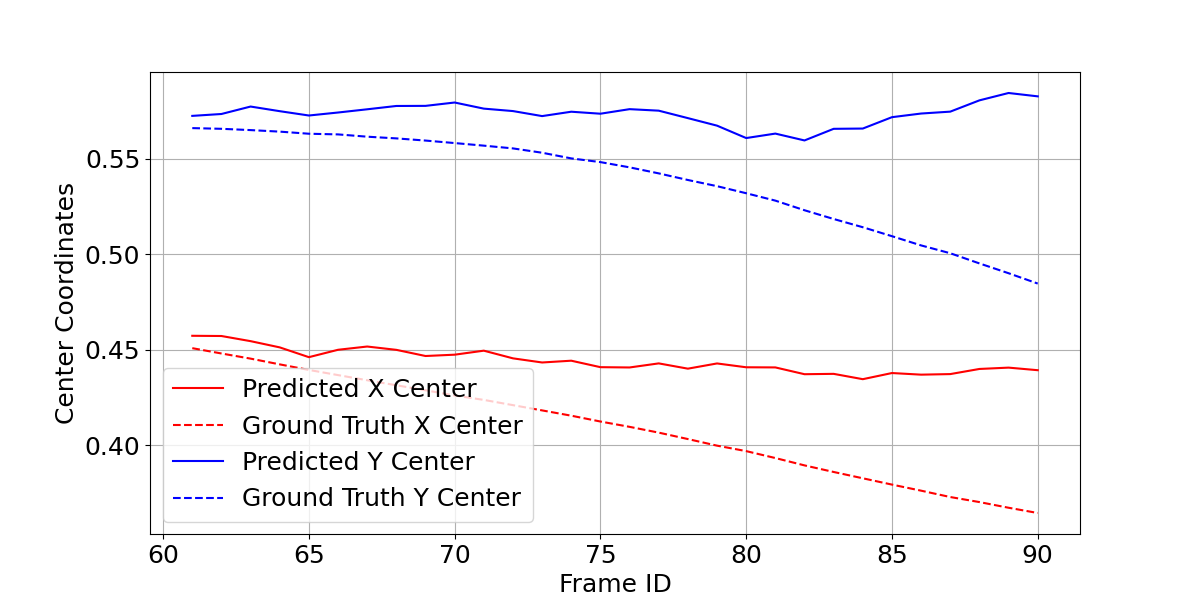
\includegraphics[width=\textwidth]{figures/framework/video_lab_platform_6 Raw Data - 1.png}
        \caption{Predictions from frame 61 to 90 without smoothing.}
        \label{fig:framework-video_lab_platform_6-1-raw}
    \end{subfigure}
    \hfill
    \begin{subfigure}[t]{0.9\textwidth}
        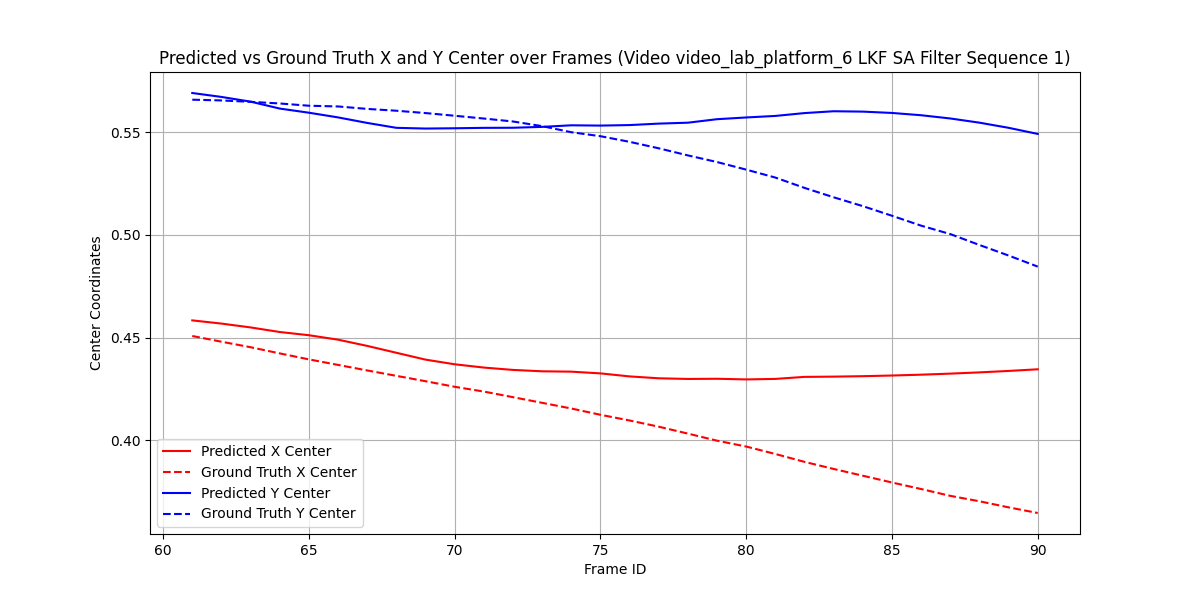
\includegraphics[width=\textwidth]{figures/framework/video_lab_platform_6 LKF SA Filter - 1.png}
        \caption{Predictions from frame 61 to 90 with Savitzky-Golay filter and Linear Kalman Filter.}
        \label{fig:framework-video_lab_platform_6-1-sa-lkf}
    \end{subfigure}
    \vfill
    \begin{subfigure}[t]{0.9\textwidth}
        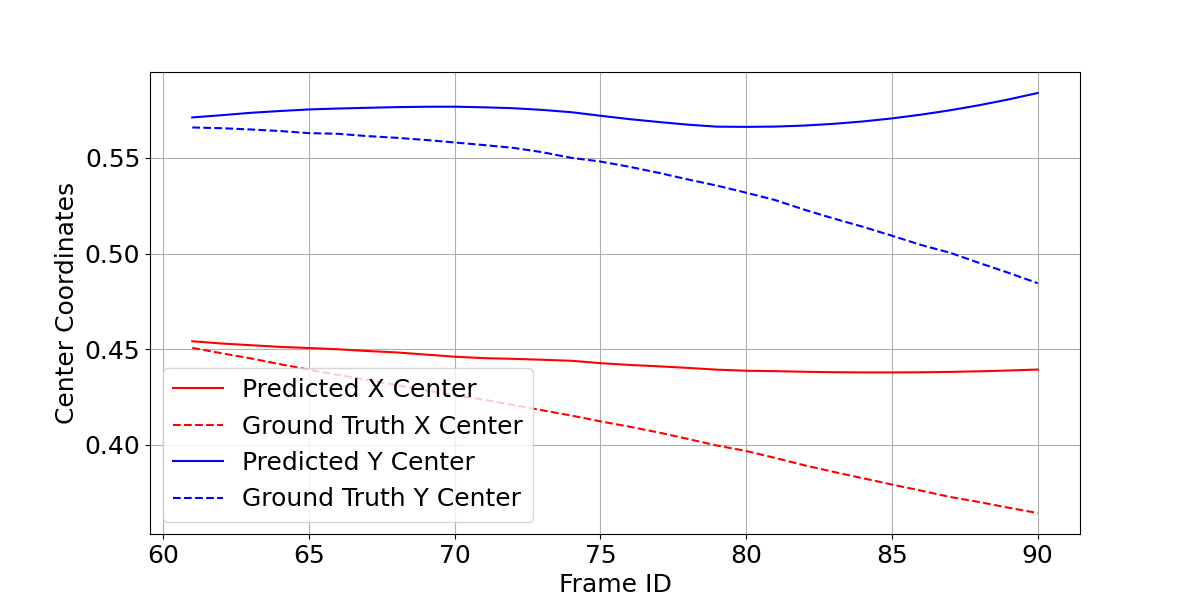
\includegraphics[width=\textwidth]{figures/framework/video_lab_platform_6 SA Filter - 1.png}
        \caption{Predictions from frame 61 to 90 with Savitzky-Golay filter.}
        \label{fig:framework-video_lab_platform_6-1-sa}
    \end{subfigure}
    \caption{Framework outputs from frame 61 to 90 for video \textit{video\_lab\_platform\_6}.}
    \label{fig:framework-video_lab_platform_6-1}
\end{figure}

\begin{figure}[H]
    \centering
    \begin{subfigure}[t]{0.9\textwidth}
        \includegraphics[width=\textwidth]{figures/framework/video_lab_platform_6 Raw Data - 2.png}
        \caption{Predictions from frame 106 to 135 without smoothing.}
        \label{fig:framework-video_lab_platform_6-2-raw}
    \end{subfigure}
    \hfill
    \begin{subfigure}[t]{0.9\textwidth}
        \includegraphics[width=\textwidth]{figures/framework/video_lab_platform_6 LKF SA Filter - 2.png}
        \caption{Predictions from frame 106 to 135 with Savitzky-Golay filter and Linear Kalman Filter.}
        \label{fig:framework-video_lab_platform_6-2-sa-lkf}
    \end{subfigure}
    \vfill
    \begin{subfigure}[t]{0.9\textwidth}
        \includegraphics[width=\textwidth]{figures/framework/video_lab_platform_6 SA Filter - 2.png}
        \caption{Predictions from frame 106 to 135 with Savitzky-Golay filter.}
        \label{fig:framework-video_lab_platform_6-2-sa}
    \end{subfigure}
    \caption{Framework outputs from frame 106 to 135 for video \textit{video\_lab\_platform\_6}.}
    \label{fig:framework-video_lab_platform_6-2}
\end{figure}

\begin{figure}[H]
    \centering
    \begin{subfigure}[t]{0.9\textwidth}
        \includegraphics[width=\textwidth]{figures/framework/video_lab_platform_6 Raw Data - 3.png}
        \caption{Predictions from frame 151 to 180 without smoothing.}
        \label{fig:framework-video_lab_platform_6-3-raw}
    \end{subfigure}
    \hfill
    \begin{subfigure}[t]{0.9\textwidth}
        \includegraphics[width=\textwidth]{figures/framework/video_lab_platform_6 LKF SA Filter - 3.png}
        \caption{Predictions from frame 151 to 180 with Savitzky-Golay filter and Linear Kalman Filter.}
        \label{fig:framework-video_lab_platform_6-3-sa-lkf}
    \end{subfigure}
    \vfill
    \begin{subfigure}[t]{0.9\textwidth}
        \includegraphics[width=\textwidth]{figures/framework/video_lab_platform_6 SA Filter - 3.png}
        \caption{Predictions from frame 151 to 180 with Savitzky-Golay filter.}
        \label{fig:framework-video_lab_platform_6-3-sa}
    \end{subfigure}
    \caption{Framework outputs from frame 151 to 180 for video \textit{video\_lab\_platform\_6}.}
    \label{fig:framework-video_lab_platform_6-3}
\end{figure}

\begin{figure}[H]
    \centering
    \begin{subfigure}[t]{0.9\textwidth}
        \includegraphics[width=\textwidth]{figures/framework/test_indoor1 Raw Data - 1.png}
        \caption{Predictions from frame 61 to 90 without smoothing.}
        \label{fig:framework-test_indoor1-1-raw}
    \end{subfigure}
    \hfill
    \begin{subfigure}[t]{0.9\textwidth}
        \includegraphics[width=\textwidth]{figures/framework/test_indoor1 LKF SA Filter - 1.png}
        \caption{Predictions from frame 61 to 90 with Savitzky-Golay filter and Linear Kalman Filter.}
        \label{fig:framework-test_indoor1-1-sa-lkf}
    \end{subfigure}
    \vfill
    \begin{subfigure}[t]{0.9\textwidth}
        \includegraphics[width=\textwidth]{figures/framework/test_indoor1 SA Filter - 1.png}
        \caption{Predictions from frame 61 to 90 with Savitzky-Golay filter.}
        \label{fig:framework-test_indoor1-1-sa}
    \end{subfigure}
    \caption{Framework outputs from frame 61 to 90 for video \textit{test\_indoor1}.}
    \label{fig:framework-test_indoor1-1}
\end{figure}

\begin{figure}[H]
    \centering
    \begin{subfigure}[t]{0.9\textwidth}
        \includegraphics[width=\textwidth]{figures/framework/test_indoor1 Raw Data - 2.png}
        \caption{Predictions from frame 106 to 135 without smoothing.}
        \label{fig:framework-test_indoor1-2-raw}
    \end{subfigure}
    \hfill
    \begin{subfigure}[t]{0.9\textwidth}
        \includegraphics[width=\textwidth]{figures/framework/test_indoor1 LKF SA Filter - 2.png}
        \caption{Predictions from frame 106 to 135 with Savitzky-Golay filter and Linear Kalman Filter.}
        \label{fig:framework-test_indoor1-2-sa-lkf}
    \end{subfigure}
    \vfill
    \begin{subfigure}[t]{0.9\textwidth}
        \includegraphics[width=\textwidth]{figures/framework/test_indoor1 SA Filter - 2.png}
        \caption{Predictions from frame 106 to 135 with Savitzky-Golay filter.}
        \label{fig:framework-test_indoor1-2-sa}
    \end{subfigure}
    \caption{Framework outputs from frame 106 to 135 for video \textit{test\_indoor1}.}
    \label{fig:framework-test_indoor1-2}
\end{figure}

\begin{figure}[H]
    \centering
    \begin{subfigure}[t]{0.9\textwidth}
        \includegraphics[width=\textwidth]{figures/framework/test_indoor1 Raw Data - 3.png}
        \caption{Predictions from frame 151 to 180 without smoothing.}
        \label{fig:framework-test_indoor1-3-raw}
    \end{subfigure}
    \hfill
    \begin{subfigure}[t]{0.9\textwidth}
        \includegraphics[width=\textwidth]{figures/framework/test_indoor1 LKF SA Filter - 3.png}
        \caption{Predictions from frame 151 to 180 with Savitzky-Golay filter and Linear Kalman Filter.}
        \label{fig:framework-test_indoor1-3-sa-lkf}
    \end{subfigure}
    \vfill
    \begin{subfigure}[t]{0.9\textwidth}
        \includegraphics[width=\textwidth]{figures/framework/test_indoor1 SA Filter - 3.png}
        \caption{Predictions from frame 151 to 180 with Savitzky-Golay filter.}
        \label{fig:framework-test_indoor1-3-sa}
    \end{subfigure}
    \caption{Framework outputs from frame 151 to 180 for video \textit{test\_indoor1}.}
    \label{fig:framework-test_indoor1-3}
\end{figure}

\newpage

Figures~\ref{fig:framework-video_lab_platform_6-1},
\ref{fig:framework-video_lab_platform_6-2},
\ref{fig:framework-video_lab_platform_6-3}, \ref{fig:framework-test_indoor1-1},
\ref{fig:framework-test_indoor1-2}, and \ref{fig:framework-test_indoor1-3}
illustrate the predicted and ground truth central positions of the refuelling
port across multiple frame sequences, comparing raw predictions with those
processed using the Savitzky-Golay filter and Linear Kalman Filter (LKF). The
model shows an initial alignment with the ground truth trajectories. However,
as the frame sequences progress, particularly in later frames, the predictions
begin to diverge significantly from the ground truth. This divergence is more
pronounced in the X center coordinate, suggesting that the model is
particularly sensitive to horizontal deviations and noise accumulation over
time. This trend is evident in both videos but is especially marked in the
\textit{test\_indoor1} dataset, where the model struggles to accurately track
abrupt changes in trajectory. These deviations highlight a critical limitation
in the model's ability to maintain accuracy over extended sequences, as errors
accumulate and cause a noticeable drift from the actual trajectory. The
application of the Savitzky-Golay filter and LKF, shown in subfigures (b),
significantly mitigates these issues by smoothing the trajectory and aligning
the predictions more closely with the ground truth, thereby reducing noise and
limiting the impact of cumulative errors. Although the Savitzky-Golay filter
alone, illustrated in subfigures (c), also improves prediction accuracy, the
combined approach with LKF proves more effective in maintaining stability and
accuracy, particularly in later frames where the impact of recursive error
propagation is most pronounced. This analysis underscores the importance of
advanced filtering techniques in enhancing the reliability of trajectory
predictions, particularly in recursive models where error accumulation is a
critical challenge. For instance, in the \textit{video\_lab\_platform\_6}
dataset, the smoothing techniques help to maintain a consistent trajectory,
even in the more challenging later frames where the unsmoothed predictions
exhibited significant drift. Similarly, in the \textit{test\_indoor1} dataset,
the filters help to manage abrupt trajectory changes more effectively, reducing
the sharp deviations that were prominent in the raw predictions. However, while
the application of these filters significantly enhances the model's
performance, it is important to recognise that they do not entirely eliminate
prediction errors. In both videos, some discrepancies between the predicted and
actual positions remain, particularly during complex or abrupt movements. This
suggests that while smoothing techniques are effective in improving overall
prediction stability, they cannot fully compensate for the model's inherent
limitations in handling dynamic and unpredictable changes in trajectory. 

%%%%%%%%%%%%%%%%%%%%%%%%%%%%%%%%%%%%%%%%%%%%%%%%%%%%%%%%%%%%%%%%%%%%%%%%%%%%%%%
%%%%%%%%%%%%%%%%%%%%%%%%%%%%%%%%% CONCLUSION %%%%%%%%%%%%%%%%%%%%%%%%%%%%%%%%%%
\chapter{Conclusion and Future Work}

\section{Summary}
This thesis has developed a comprehensive framework for predicting the future
positions of aircraft refuelling ports using advanced deep learning techniques.
The primary accomplishment of this project is the integration of the SizPos-GRU
model with a fine-tuned YOLOv10 object detection system. The framework
effectively captures temporal dependencies and spatial relationships within
video sequences, leading to accurate and reliable predictions of refuelling
port positions. The use of smoothing techniques, such as the Savitzky-Golay
filter combined with Linear Kalman Filter (LKF), significantly enhanced the
model’s performance, particularly in noisy and dynamic environments. The
results demonstrate that the proposed framework achieves superior predictive
accuracy compared to existing models, particularly in terms of reducing Average
Displacement Error (ADE) and Final Displacement Error (FDE), while maintaining
high spatial consistency. These outcomes underscore the potential of the
developed framework to improve the automation and safety of aircraft refuelling
operations.

\section{Technological Contributions}
This research presents several key technological contributions to the field of
automated aircraft refuelling and predictive modelling. The primary
contribution is the development of the SizPos-GRU model, which incorporates an
encoder-attention-decoder architecture tailored for capturing the complex
temporal and spatial relationships in video sequences. The integration of this
model with a fine-tuned YOLOv10 object detection system provides a robust
solution for detecting, tracking, and predicting the trajectory of refuelling
ports. Additionally, the implementation of advanced smoothing techniques, such
as the Savitzky-Golay filter in conjunction with Linear Kalman Filtering,
contributes to more stable and accurate predictions, even in challenging
environments. These technological advancements significantly enhance the
predictive capabilities of automated systems in dynamic environments, offering
practical applications in the aviation industry.

\section{Future Work}
There are several avenues for future research that could extend the findings of
this thesis. One potential direction is the exploration of more advanced deep
learning architectures, such as Transformers or hybrid models that combine the
strengths of recurrent neural networks and convolutional neural networks, to
further enhance predictive accuracy. Expanding the dataset to include a broader
range of scenarios, aircraft types, and environmental conditions could also
improve model generalization and robustness. Additionally, incorporating
multi-modal data, such as infrared or radar signals, could further enhance the
model’s performance under different environmental conditions, such as low
visibility or harsh weather. Finally, integrating this prediction framework
into a real-time system and conducting live operational testing would be
crucial steps towards practical deployment, addressing real-world challenges
such as latency, computational efficiency, and system integration.
%TC:ignore 
\appendix

%TC:endignore 

\bibliographystyle{abbrvnat}
\bibliography{LaTeX,CUCitations}

\end{document}

